\documentclass[a4paper,11pt]{article}
\pdfoutput=1 % if your are submitting a pdflatex (i.e. if you have
             % images in pdf, png or jpg format)

\usepackage{jheppub} % for details on the use of the package, please
                     % see the JHEP-author-manual

\usepackage[T1]{fontenc} % if needed
%\usepackage[utf8]{inputenc}
\usepackage{graphicx}
\usepackage{caption}
\usepackage{subcaption}

\usepackage{hepparticles}
\usepackage{hepnames}
\usepackage{hepnicenames}

\usepackage[usenames,dvipsnames]{xcolor}
\usepackage{tikz}
\usepackage{hyperref}

\usepackage{soul}% For strikeout, use \st{text} . Can be removed from submitted manuscript

\usepackage{lineno}
\linenumbers
\usepackage{cancel}

%%%Physics, mostly
\newcommand{\overbar}[1]{\mkern 1.5mu\overline{\mkern-1.5mu#1\mkern-1.5mu}\mkern 1.5mu}
\DeclareMathOperator{\Tr}{Tr}
\DeclareMathOperator{\gev}{GeV}
\DeclareMathOperator{\mev}{MeV}

\newcommand{\fou}[1]{\ensuremath{\mathscr{F}\left[#1\right]}}
\newcommand{\infou}[1]{\ensuremath{\mathscr{F}^{-1}\left[#1\right]}}
\newcommand{\psibar}{\bar{\psi}}
\newcommand{\pbar}{\overbar{p}}
\newcommand{\ubar}{\overbar{u}}
\newcommand{\vbar}{\overbar{v}}
\newcommand{\kbar}{\overbar{k}}
\newcommand{\chibar}{\overbar{\chi}}
\newcommand{\MG}{M{\footnotesize AD}G{\footnotesize RAPH}5}
\newcommand{\FNMG}{{\footnotesize M}{\tiny AD}{\footnotesize G}{\tiny RAPH} }
\newcommand{\PYTHIA}{P{\footnotesize YTHIA} }
\newcommand\T{\rule{0pt}{2.6ex}}       % Top strut
\newcommand\B{\rule[-1.2ex]{0pt}{0pt}} % Bottom strut

\newcommand{\tr}[1]{\Tr\left[#1\right]}

\makeatother % End of region containing @ commands
\renewcommand{\labelenumi}{(\alph{enumi})} % Use letters for enumerate
 \DeclareMathOperator{\Sample}{Sample}
\let\vaccent=\v % rename builtin command \v{} to \vaccent{}
\renewcommand{\v}[1]{\ensuremath{\mathbf{#1}}} % for vectors
\newcommand{\gv}[1]{\ensuremath{\mbox{\boldmath$ #1 $}}} 
% for vectors of Greek letters
\newcommand{\e}[1]{\ensuremath{\times 10^{#1}}}
\newcommand{\uv}[1]{\ensuremath{\mathbf{\hat{#1}}}} % for unit vector
\newcommand{\abs}[1]{\left| #1 \right|} % for absolute value
\newcommand{\avg}[1]{\left< #1 \right>} % for average
\let\underdot=\d % rename builtin command \d{} to \underdot{}
\renewcommand{\d}[2]{\frac{d #1}{d #2}} % for derivatives
\newcommand{\dd}[2]{\frac{d^2 #1}{d #2^2}} % for double derivatives
\newcommand{\pd}[2]{\frac{\partial #1}{\partial #2}} 
% for partial derivatives
\newcommand{\pdd}[2]{\frac{\partial^2 #1}{\partial #2^2}} 
% for double partial derivatives
\newcommand{\pdn}[3]{\frac{\partial^#1 #2}{\partial #3^#1}}
\newcommand{\pdh}[1]{\frac{\partial}{\partial #1}}   %things like d/dt, 
\newcommand{\eval}[1]{\left< #1 \right>}
\newcommand{\pdc}[3]{\left( \frac{\partial #1}{\partial #2}
 \right)_{#3}} % for thermodynamic partial derivatives
\newcommand{\ket}[1]{\left| #1 \right>} % for Dirac bras
\newcommand{\bra}[1]{\left< #1 \right|} % for Dirac kets
\newcommand{\braket}[2]{\left< #1 \vphantom{#2} \right|
 \left. #2 \vphantom{#1} \right>} % for Dirac brackets
\newcommand{\matrixel}[3]{\left< #1 \vphantom{#2#3} \right|
 #2 \left| #3 \vphantom{#1#2} \right>} % for Dirac matrix elements
\newcommand{\grad}[1]{\gv{\nabla} #1} % for gradient
\let\divsymb=\div % rename builtin command \div to \divsymb
\renewcommand{\div}[1]{\gv{\nabla} \cdot #1} % for divergence
\newcommand{\curl}[1]{\gv{\nabla} \times #1} % for curl
\let\baraccent=\= % rename builtin command \= to \baraccent
\renewcommand{\=}[1]{\stackrel{#1}{=}} % for putting numbers above =
\newtheorem{prop}{Proposition}
\newtheorem{thm}{Theorem}[section]
\newtheorem{lem}[thm]{Lemma}

\newcommand{\question}[1]{\textcolor{red}{#1}}%For comments
\newcommand{\comm}[1]{\textcolor{magenta}{#1}}%For comments
\newcommand{\draft}[1]{\textcolor{blue}{#1}}%For comments

\newcommand{\fg}[1]{\textcolor{ForestGreen}{#1}}   % to avoid writing ForestGreen all the freaking time

\tikzstyle arrowformat=[scale=1.5]
\tikzstyle scalar =[dashed]
\tikzstyle mom=[draw=blue]
\tikzset{
gluon/.style={decorate, draw=black, decoration={coil, amplitude = 3.5pt, segment length=4.8pt}},
photon/.style={decorate, draw=black, decoration={snake=coil, amplitude = 2pt, segment length=9pt}},
zbo/.style={decorate, draw=black, decoration={snake=coil}},
fermion/.style={draw=black, postaction={decorate}, decoration={markings, mark = at position 0.55 with {\arrow[arrowformat]{>}}}},
antifermion/.style={draw=black, postaction={decorate}, decoration={markings, mark = at position 0.55 with {\arrow[arrowformat]{<}}}}
}
\usetikzlibrary{patterns}
\usetikzlibrary{arrows}
\usetikzlibrary{decorations.pathmorphing,decorations.markings, decorations.pathreplacing, trees}

\title{\boldmath Draft: Constraints on Simplified Dark Matter Models using Mono-X Collider Searches}


%% %simple case: 2 authors, same institution
%% \author{A. Uthor}
%% \author{and A. Nother Author}
%% \affiliation{Institution,\\Address, Country}

% more complex case: 4 authors, 3 institutions, 2 footnotes
\author[a,1]{Amelia J. Brennan,\note{Corresponding author.}}
\author[b]{Johanna Gramling,}
\author[b]{Thomas Jacques,}
\author[a]{and Millie F. McDonald}

% The "\note" macro will give a warning: "Ignoring empty anchor..."
% you can safely ignore it.

\affiliation[a]{The University of Melbourne, Parkville 3010, Australia}
\affiliation[b]{Universit\'{e} de Gen\`{e}ve, Quai E. Ansermet 24, 1211 Gen\`{e}ve 4, Switzerland}

% e-mail addresses: one for each author, in the same order as the authors
\emailAdd{a.brennan@student.unimelb.edu.au}
\emailAdd{johanna.gramling@cern.ch}
\emailAdd{thomas.jacques@unige.ch}
\emailAdd{milliem@student.unimelb.edu.au}

\abstract{Abstract...}

\begin{document} 
\maketitle
\flushbottom

% Keep this section clean - create a new input tex file in sections/ if a new section is required, and add it here.

%\section{Checking some latex commands}
%\label{sec:intro}
%% !TEX root = ../paper.tex

The first simplified model considered here comprises a Dirac fermion DM particle (labeled $\chi$), coupled to SM quarks via an $s$-channel vector mediator (labeled $\xi$). The couplings of the mediator to the quark pair and DM pair are denoted $g_q$ and $g_{\chi}$ respectively, and are assumed to be equal, that is, $g_q = g_{\chi}$. The width of the vector mediator is variable by hand, and in the following study three indicative widths will be used.


\begin{flushleft}
Amelia, Johanna and Thomas: Anything in \textcolor{red}{red} (\textcolor{magenta}{magenta}) is a question (comment) regarding content and anything in \textcolor{blue}{blue} is incomplete/not ideally worded.
\end{flushleft}

\begin{flushleft}
\comm{Thanks, this looks great so far! I've gone through and made a few changes to the theory section, but ran out of time, there's still quite a bit more for me to add. Could people please sign their initials on their comments so we can keep track of who's saying what?  -Tom}
\end{flushleft}

\begin{flushleft}
\textcolor{ForestGreen}{FYI - bits in green are what I've added, I'll drop the colour once others have had a chance to see (and because some of my sentences could maybe use rewriting). - Amelia}
\end{flushleft}

\section{Introduction} 
\label{sec:sec1}
% !TEX root = ../new_paper.tex

Simplified models have emerged as a powerful tool for the interpretation of collider, direct and indirect detection signals of dark matter (DM). Previously,  searches for DM were conducted within the context of both Effective Field Theories (EFTs) \cite{Aad:1363019, ATLAS-CONF-2012-147, CMS-PAS-EXO-12-048, Buckley:2013jwa, Abdallah:1472683, MonoZ, MonoX} and full UV-complete theories like Supersymmetry \cite{ComppMSSM, Aad:2012ms, Aad:2012fqa, Aad:2014wea, SUSY_official_paper} and extra dimensions \cite{}. The latter approach, though well-motivated, is typified by a broad parameter space and generally yields results which are insensitive to the wider class of DM models. EFT constraints, in comparison, are applicable to a broad range of models and rely on the specification of only a small set of parameters, namely the suppression scale, $\Mstar$ and the DM mass, $\mDM$ \cite{}.
%This prescription however is known to be problematic in high-energy scenarios \cite{}, where the underlying simplification becomes invalid.
%\bigskip
In the EFT framework, interactions between the dark and Standard Model (SM) sector are parametrised by a set of higher-dimensional effective operators \cite{}. These operators arise when the mass of the mediating particle is assumed to be significantly larger than the momentum transferred, $\mathcal{Q}_{t}$, in a given interaction \cite{}. Where this is not the case, the EFT prescription can produce constraints which detour dramatically from those of the associated UV-complete model \cite{Bai:2010hh, DMCons2, Fox:2011fx, Graesser:2011vj, An:2011ck}. This is not so important in direct detection experiments where the momentum transferred in the scattering of DM particles with heavy nuclei is generally of the order of tens of keV \cite{EFTDM, DMCons3}. Similarly, in indirect searches the annihilations of non-relativistic DM particles in the galactic halo occur with momentum transfers on the order of $\mDM$ \cite{}. However, for collider searches - where the accessible center of mass energy of two colliding baryons may be sufficient to produce the mediator on-shell - the range of validity of the EFT prescription is significantly diminished \cite{}. Indeed, recent works have shown the EFT approach to be unreliable in certain cases for the interpretation of data collected during the $\sqrt{\hat{s}} =$ 8 TeV Run I of the Large Hadron Collider (LHC) \cite{}. In light of this, simplified models (SiMs) have become the preferred tool for the interpretation of collider DM searches \cite{Harris:2014hga, Buchmueller:2014yoa}.
%\bigskip

In a nutshell, a simplified model arises when the heavy mediator which was integrated out in the EFT framework is reintroduced. Like EFTs, simplified models admit the comparison of results obtained in the different avenues of dark matter study \cite{} and are defined by a relatively small set of parameters - namely $\mDM$, the mass of the mediator, $\Mmed$, and the SM-mediator and DM-mediator coupling strengths, $\gq$ and $\gX$. Unlike EFTs, constraints calculated within the context of a simplified model are valid across a broad energy range ($\mathcal{O}$(GeV-TeV)).
%, removing the question of validity of the EFT approximation \cite{}.
%\bigskip

To date, very few analyses include a dedicated study of any simplified models of DM. This is generally because the focus in DM collider searches at both ATLAS and CMS has been on generic EFT models. The recent release of several reports and recommendations on simplified models for the LHC $[$DM forum report, other SiMs paper$]$ indicate that they are expected to play a more prominent role in Run II. The aim of this work, then, is to investigate a phenomenologically distinct set of simplified models likely to be included in Run II searches, and to constrain these using results already publicly available. In particular, constraints are placed on the simplified models corresponding to the simplest UV-completions in the $s$-channel of the D5 (vector) and D8 (axial-vector) effective operators\footnote{The D5 and D8 operators form a nice starting point in the analysis of simplified models as they have been studied exhaustively in the past (see Ref. \cite{}). This attention is motivated by the fact that collider limits for the D5 (D8) operator can be readily transformed into limits on spin-independent (spin-dependent) DM-nucleon scattering and vice versa. With the exception of D1 (see sec. \ref{section}), and D9 and D11 (which have no simple simplified model counterparts \cite{}), the remaining effective operators induce elastic scattering which is suppressed by powers of the DM velocity or the momentum transferred \cite{Kumar}. Hence, these operators are largely ignored in the literature.}. We also include a case with mediator exchange in the $t$-channel, which approaches the vector EFT model in the heavy-mediator limit, but remains kinematically distinct from its $s$-channel counterpart.

We constrain these models using public results from \monoX + missing transverse energy ($\met$) searches conducted by the ATLAS Collaboration. In particular, we focus on searches where X is either a parton (appearing as a narrow-radius jet), a leptonically-decaying $Z$ boson, or a hadronically-decaying $W$ or $Z$ boson (appearing as a large-radius jet). The purpose of this approach is both to enhance and update existing simplified model limits \cite{}, using the full 20.3 $fb^{-1}$ of Run I ATLAS data, and extend the range of phase space considered both in mass and relative strength of the couplings to the SM and DM sectors. We also aim to provide a cross-check and comparison of the performance of the three channels; while the \monojet channel is expected to be most sensitive, the inclusion of two additional channels could enhance the limits in combination. Further, we extend the study of simplified models by allowing the width of the mediator and the SM-/DM-mediator couplings to vary, which previously have often been treated as fixed quantities \cite{}. We also include a comparison of collider limits with relic density constraints and limits from direct detection experiments.

The remainder of the paper is organised as follows. Section \ref{sec:sec2} contains a compendium of the simplified models chosen for analysis. Section \ref{sec:sec3} outlines the technique used to convert \monoX + $\met$ limits on the visible cross-section for any new physics process into constraints on simplified models, specifically, the couplings $\gq$ and $\gX$. Lastly, the results are presented in Section \ref{sec:sec4} along with a discussion of the implications of this work. Appendices \ref{Appendix_limitsetting} and \ref{Appendix_validation} cover the details of our limit setting procedure and analyses validation.
%\textcolor{magenta}{This section should include:}
%\begin{enumerate}
%\item \textcolor{magenta}{Motivation for SiMs: limited validity of EFTs \& uneconomically broad parameter space of full UV-complete models/insensitivity of model-dependent results to the wider class of DM models $\rightarrow$ advantage of simplified models (relatively small parameter space, predictions accurate and complementary across a broad energy range $\mathcal{O}$(GeV-TeV)).\footnote{\textcolor{red}{Are we assuming that the reader understands the basics of a "simplified model"? Or should we have one or two sentences that summarise the differences between, say, an EFT and a SiM?}}}
%\item \textcolor{magenta}{Brief description of the aim of the analysis (e.g. something like "to apply constraints to $\mX$, $\mMed$ and $\gq = \gX = f$ for four phenomenologically distinct simplified models, etc) along with a brief motivation for the choice of simplified models\footnote{\textcolor{red}{Or should this part be in section \ref{sec:sec2}?}}.}
%\item \textcolor{magenta}{Summary of content of paper (eg. "This paper is organised as follows: section 2 is a compendium of the simplified models chosen for analysis..." etc)}
%\end{enumerate}


\section{Simplified Models of Dark Matter} 
\label{sec:sec2}
% !TEX root = ../new_paper.tex
\subsection{Model Descriptions}
We begin with a short set of assumptions: that the DM particle, $\chi$, is a weakly interacting Dirac fermion, that it is a singlet under the SM, and that it is the lightest stable new particle.
\iffalse
(\comm{Not sure if this is relevant anymore, if we've ditched the scalar model. - Mia})
\fi
Additionally the new sector is assumed to couple only to the SM quarks; while possible coupling to SM leptons e.g. \cite{Fox:2011fx} or gluons e.g. \cite{SiM_gluons} has been studied elsewhere, it is beyond the scope of this paper. The nature of the mediating particle then results from these assumptions: in the $s$-channel it is chosen to be a vector particle which must also be a SM singlet, denoted $\xi$, while in the $t$-channel it is a scalar particle which is necessarily charged and coloured, and labelled $\phi$.

The $s$-channel models chosen for analysis are characterised by vector ($sV$) or axial-vector ($sA$) couplings to both the dark and SM sectors. They are described by the following interaction Lagrangians:
\begin{equation}
\label{L_int_sV}
\mathcal{L}_{sV} \supset - \xi_{\mu}\left[ \sum\limits_{q} \gq\bar{q}\gamma^{\mu}q - \gX\bar{\chi}\gamma^{\mu}\chi\right],
\end{equation}
\begin{equation}
\label{L_int_sA}
\mathcal{L}_{sA} \supset  \xi_{\mu}\left[\sum\limits_{q} \gq\bar{q}\gamma^{\mu}\gamma_{5}q - \gX\bar{\chi}\gamma^{\mu}\gamma_{5}\chi\right],
\end{equation}
%\begin{equation}
%\label{L_int_sS}
%\mathcal{L}_{sS} = \sum\limits_{i=1}^{6} g_{q_i}\bar{q_i}q_i\eta + \gX\bar{\chi}\chi\eta,
%\end{equation}
where the sum is over all quarks.
\iffalse
\st{where the sum is over all quarks, $\xi$ is the (axial-)vector mediator and $\chi$ is the dark matter particle - a weakly interacting SM singlet Dirac fermion with mass $\mX$.}
\fi
%\question{The scalar model should really have a Yukawa coupling (ie $\gq \rightarrow \gq m_q / v$) if we want to be consistent with D1 and the ATLAS/CMS run2 simplified models. Is it too late to implement this? - Tom.} \comm{I agree, and this should be easy enough to implement I think. - Amelia}
%\st{For simplicity, it is assumed that both $\xi$ and $\eta$ are SM singlet particles and couple only to pair-antipair combinations of $\chi$ and the SM quarks, with coupling strengths $\gX$ and $\gq$ respectively.}
For the couplings $\gq$ and $\gX$ to remain within the perturbative regime, they are required to satisy $\gq,\gX \leq 4\pi$, though stronger perturbativity requirements do exist \cite{ValidEFT}.
%\bigskip

%\st{Finally, for convenience, the mediator is assumed to couple to }$\cancel{\chi}$\st{ with the same strength as to each of the six quarks, that is, }$\cancel{\gq = \gX \equiv f}$. \comm{Removed, since we want to include cases where this isn't true! - Amelia}
%Note that the vector and axial-vector models have already been studied extensively \cite{Buchmueller:2014yoa, Chatrchyan:2013qha, Aad:2012hf, Harris:2014hga} and so serve as a good basis for the comparison of constraints. \comm{I need to add some citations for the scalar model here - Tom}

The $t$-channel model (abbreviated $tS$) is primarily
%characterised by a scalar mediator and is
motivated by analogy with a common aspect of Supersymmetric models: neutralino DM interacting with the SM sector via $t$-channel exchange of a squark \cite{SUSYDM}. Note that in this Supersymmetric scenario the DM particle is a Majorana fermion. The collider phenomenology of a SiM in which $\chi$ is of Majorana type is kinematically identical to the corresponding Dirac case (requiring multiplication of the cross-section by a simple factor in order to compute limits) and so Majorana DM is not covered here\footnote{The exception being in the validation of the \monoZ channel, see Sec. \ref{monoZ_validation}.}. The exception to this rule is the $s$-channel vector mediator model, which vanishes if $\chi$ is a Majorana fermion \cite{METSig}.
%\bigskip

In the $tS$ model, the mediator is allowed to couple to either the left or right-handed quarks as an SU(2) doublet or singlet respectively. Since the LHC is insensitive to the chirality of the quarks, we assume for simplicity that $\phi$ couples to the left-handed quarks only, and is itself an SU(2) doublet, allowing radiation of a $W$ boson. To avoid different couplings to quarks of different generations, and to remain in step with the DM forum recommendations \cite{DMForumReport}, we include three generations of mediator doublets $\phi_i$, with equal masses and couplings. The interaction Lagrangian for this model is then:
\begin{equation}
\label{L_int_tS}
\mathcal{L}_{tS} \supset \sum_{i} \gqX \bar{Q_i} P_R \phi_i \chi + {\rm h.c.},
\end{equation}
where the sum is over the three quark doublets, $\gqX$ is the DM-quark coupling (equal for each generation), and $P_R$ is the usual chiral projection operator.

\subsection{The Mono-$X$ + $\met$ Signature}
The \monoX + $\met$ signal (abbreviated to mono-$X$) is a popular collider signal in the search for new physics, particularly in the search for dark matter. Since DM particles are not expected to interact with detector material, they appear as missing transverse energy when balanced against a visible object, $X$, that is radiated from the initial or intermediate state. %(where the latter is permitted in the $t$-channel model).
For the $s$-channel SiMs discussed above, only initial-state radiation is permitted; see figs.~\ref{fig:FD_sV_gluonISR} and \ref{fig:FD_sV_WZISR} for examples. For the $tS$ model, radiation of a gluon or electroweak (EW) boson is permitted both from initial state partons (fig.~\ref{fig:FD_tS_gluonISR}) or from the mediator (fig.~\ref{fig:FD_tS_WZmediator}).

The most likely scenario at the LHC is production of a jet alongside the invisible $\chi$ pair, as a result of the strong coupling and prevalence of partons in the initial state. However, to fully exploit the potential of the ATLAS detector to record and identify a vast array of particle types, we also consider two additional channels. Firstly, we take advantage of the relative cleanliness and simplicity of leptons in the leptonically-decaying mono-$Z(\rightarrow \ell^+ \ell^-)$ channel. We also take advantage of the large hadronic branching fraction, and developing jet-identification techniques for boosted EW bosons, in the hadronically-decaying mono-$W/Z(\rightarrow jj)$ channel\footnote{In addition, one of the first Run II dark matter search results from ATLAS was from this channel \cite{monoWZ_run2}, released during the preparation of this paper.}. In both cases, the large multi-jet background is reduced, and complications in jet production such as parton-matching can be ignored, making these an interesting alternative to the \monojet channel where speed, efficiency and a reduction in jet-associated uncertainties may make up for a loss in sensitivity.

%, which may then enhance the limit in combination with monojet processes.}

% Note for figure: putting spaces between the \end{subfig} and the next begin{subfig} leads to the figures stacking rather than sitting side-by-side, don't want this!
% Also, have deliberately set TSD plots to width = 0.4, with horizontal space in the middle, to get the relative sizes of the figures looking correct.
\begin{figure}[t]
  \centering
  \begin{subfigure}[b]{0.45\textwidth}
    \centering
    \resizebox{\linewidth}{!}{
      \begin{tikzpicture}
        \draw[fermion] (-1.5,1.5)node[left]{$q$} --(-0.75,0.75);
        %\draw[dashed] (-0.75,0.75) -- (0,1.5)node[right]{$j$}; %\draw[dashed] (-0.75,0.75) --  (0,1.5)node[right]{X};
        \draw[gluon] (-0.75,0.75) -- (0,1.5)node[right]{$g$};
        \draw[fermion] (-0.75,0.75) -- (0,0);
        \draw[antifermion] (-1.5,-1.5)node[left]{$\bar{q}$} --(0,0);
        \draw[fill] (0,0) circle [radius=0.0]node[left]{$\gq\mbox{ }$};
        \draw[photon] (0,0) --node[above]{$\xi$} (2,0);
        \draw[fermion] (2,0) -- (3.5,1.5)node[right]{$\chi$};
        \draw[antifermion] (2,0) --(3.5,-1.5)node[right]{$\bar{\chi}$};
        \draw[fill] (2,0) circle [radius=0.0]node[right]{$\mbox{ }\gX$};
      \end{tikzpicture}
    }
    \caption{}
    \label{fig:FD_sV_gluonISR}
  \end{subfigure}
  \begin{subfigure}[b]{0.45\textwidth}
    \centering
    \resizebox{\linewidth}{!}{
      \begin{tikzpicture}
        \draw[fermion] (-1.5,1.5)node[left]{$q$} --(-0.75,0.75);
        \draw[photon] (-0.75,0.75) -- (0,1.5)node[right]{$W/Z$}; %\draw[dashed] (-0.75,0.75) -- (0,1.5)node[right]{X};
        \draw[fermion] (-0.75,0.75) -- (0,0);
        \draw[antifermion] (-1.5,-1.5)node[left]{$\bar{q}$} --(0,0);
        \draw[fill] (0,0) circle [radius=0.0]node[left]{$\gq\mbox{ }$};
        \draw[photon] (0,0) --node[above]{$\xi$} (2,0);
        \draw[fermion] (2,0) -- (3.5,1.5)node[right]{$\chi$};
        \draw[antifermion] (2,0) --(3.5,-1.5)node[right]{$\bar{\chi}$};
        \draw[fill] (2,0) circle [radius=0.0]node[right]{$\mbox{ }\gX$};
      \end{tikzpicture}
    }
    \caption{}
    \label{fig:FD_sV_WZISR}
  \end{subfigure}
  \begin{subfigure}[b]{0.4\textwidth}
    \centering
    \resizebox{\linewidth}{!}{
      \begin{tikzpicture}
        \draw[fermion] (-2,1.)node[left]{$q$} --(-1,1.);
        \draw[fermion] (-1,1.) --(0,1.);
        \draw[gluon] (-1,1.) --(0,2.)node[right]{$g$};
        \draw[antifermion] (-2,-1)node[left]{$\bar{q}$} --(0,-1);
        \draw[fill] (0,1.) circle [radius=0.0]node[above]{$\gqX$};
        \draw[dashed] (0,1.) -- node[left]{$\phi_{q}$}(0,-1);
        \draw[fermion] (0,1.) -- (2,1.)node[right]{$\chi$};
        \draw[antifermion] (0,-1) --(2,-1)node[right]{$\bar{\chi}$};
        \draw[fill] (0,-1) circle [radius=0.0]node[below]{$\gqX$};
      \end{tikzpicture}
    }
    \caption{}
    \label{fig:FD_tS_gluonISR}
  \end{subfigure}
  \hspace{1cm}
  \begin{subfigure}[b]{0.4\textwidth}
    \centering
    \resizebox{\linewidth}{!}{
      \begin{tikzpicture}
        \draw[fermion] (-2,1.)node[left]{$q$} --(0,1.);
        \draw[antifermion] (-2,-1)node[left]{$\bar{q}'$} --(0,-1);
        \draw[fill] (0,1.) circle [radius=0.0]node[above]{$\gqX$};
        \draw[dashed] (0,1.) -- node[left]{$\phi_{q}$}(0,0.25);
        \draw[photon] (0,0.) -- (1.5, 0.)node[right]{$W/Z$};
        \draw[dashed] (0,0.) -- node[left]{$\phi_{q'}$}(0,-1);
        \draw[fermion] (0,1.) -- (2,1.)node[right]{$\chi$};
        \draw[antifermion] (0,-1) --(2,-1)node[right]{$\bar{\chi}$};
        \draw[fill] (0,-1) circle [radius=0.0]node[below]{$\gqX$};
      \end{tikzpicture}
    }
    \caption{}
    \label{fig:FD_tS_WZmediator}
  \end{subfigure}
%  \begin{subfigure}[b]{0.45\textwidth}
%    \centering
%    \begin{tikzpicture}
%      \draw[fermion] (-1.5,1.5)node[left]{$q$} --(0,0);
%      \draw[gluon] (-1.5,-1.5)node[left]{$g$} --(0,0);
%      %\draw[fill] (0,0) circle [radius=0.05]node[left]{$g_{q'}\mbox{ }$};
%      \draw[fill] (0,0) circle [radius=0.0]node[left]{$\mbox{ }$};
%      \draw[fermion] (0,0) --node[above]{$q$} (2,0);
%      \draw[photon] (2,0) -- node[above]{$\xi\mbox{\textcolor{white}{m}}$}(2.75,0.75);
%      \draw[fermion] (2.75,0.75) -- (3.5,1.5)node[right]{$\chi$};
%      \draw[antifermion] (2.75,0.75) --(3.5,0)node[right]{$\bar{\chi}$};
%      \draw[fill] (2,0) circle [radius=0.0]node[below]{$\gq\mbox{ }$};
%      \draw[fermion] (2,0) --(3.5,-1.5)node[right]{$q$};
%      \draw[fill] (2.75,0.75) circle [radius=0.0]node[right]{$\mbox{\textcolor{white}{\tiny m}}\gX$};
%    \end{tikzpicture}
%    \caption{}
%    \label{Signal_phen_sd}
%  \end{subfigure}
%  \begin{subfigure}[b]{0.45\textwidth}
%    \centering
%    \begin{tikzpicture}
%      \draw[gluon] (-1.5,1.5)node[left]{$g$} --(0,0);
%      \draw[gluon] (-1.5,-1.5)node[left]{$g$} --(0,0);
%      %\draw[fill] (0,0) circle [radius=0.05]node[left]{$g_{q'}\mbox{ }$};
%      \draw[fill] (0,0) circle [radius=0.0]node[left]{$\mbox{ }$};
%      \draw[gluon] (0,0) -- (1,0);
%      \draw[antifermion] (1,0) -- node[above]{$\bar{q}\mbox{\textcolor{white}{m}}$}(1.75,0.75);
%      \draw[photon] (1.75,0.75) -- node[above]{$\xi\mbox{\textcolor{white}{m}}$}(2.5,1.5);
%      \draw[fermion] (2.5, 1.5) -- (3.25, 2.25)node[right]{$\chi$};
%      \draw[antifermion] (2.5, 1.5) -- (3.25, 0.75)node[right]{$\bar{\chi}$};
%      \draw[antifermion] (1.75,0.75) --(2.5,0)node[right]{$\bar{q}$};
%      %\draw[fill] (2,0) circle [radius=0.0]node[below]{$\gq\mbox{ }$};
%      \draw[fermion] (1,0) --(2.5,-1.5)node[right]{$q$};
%      \draw[fill] (1.75,0.75) circle [radius=0.0]node[right]{$\mbox{\textcolor{white}{\tiny m}}\gq$};
%      \draw[fill] (2.5,1.5) circle [radius=0.0]node[right]{$\mbox{\textcolor{white}{\tiny m}}\gX$};
%    \end{tikzpicture}
%    \caption{}
%    \label{Signal_phen_sd}
%  \end{subfigure}
%  \begin{subfigure}[b]{0.4\textwidth}
%    \centering
%    \resizebox{\linewidth}{!}{
%      \begin{tikzpicture}
%        \draw[fermion] (-2,1.)node[left]{$q$} --(0,1.);
%        \draw[antifermion] (-2,-1)node[left]{$\bar{q}$} --(0,-1);
%        \draw[dashed] (0,1.) -- (0,-1);
%        \draw[fermion] (0,1.) -- (2,1.)node[right]{$\chi$};
%        \draw[antifermion] (0,-1) --(2,-1)node[right]{$\bar{\chi}$};
%      \end{tikzpicture}
%    }
%    \caption{}
%    %\label{Signal_phen_tg}
%  \end{subfigure}
%  \begin{subfigure}[b]{0.4\textwidth}
%    \centering
%    \resizebox{\linewidth}{!}{
%      \begin{tikzpicture}
%        \draw[fermion] (-1.5,1.5)node[left]{$q$} --(0,0);
%        \draw[antifermion] (-1.5,-1.5)node[left]{$\bar{q}$} --(0,0);
%        \draw[dashed] (0,0) -- (2,0);
%        \draw[fermion] (2,0) --(3.5,1.5)node[right]{$\chi$};
%        \draw[antifermion] (2,0) --(3.5, -1.5)node[right]{$\bar{\chi}$};
%      \end{tikzpicture}
%    }
%    \caption{}
%    %\label{Signal_phen_tg}
%  \end{subfigure}
  \caption{Representative dark matter pair-production processes with a gluon or $W/Z$ boson in the final state for the $s$-channel (a,b) and $t$-channel (c,d) models.}
  \label{allchannel_sig_phen}
\end{figure}

%previously had a footnote: It is worth noting here that the mono-$W$ channel has previously been chosen for its apparent ability to distinguish a case where $u$- and $d$-type quarks couple with opposite sign to the new physics sector \cite{}\comm{(Tait)}. However, during the preparation of this paper this has been shown to be an unphysical scenario \cite{}\comm{(Bell, Leane)}
%\bigskip

\subsection{Mass and Coupling Points}  % Moved from section 3
A representative set of dark matter and mediator masses, listed in table \ref{Mass_coup_points}, are chosen for study in each detection channel. DM masses of 3, 30 and 300 GeV are also included in the \monoZ channel, where ease of production permits higher granularity. All $(\mX, \Mmed)$ combinations are allowed in the $sV$ and $sA$ models, while in the $tS$ model $\Mmed$ must be greater than $\mX$ to ensure stability of the DM particle. The couplings $\gq$ and $\gqX$ are set to unity, while the DM-mediator coupling in the $s$-channel models, $\gX$, is varied from 0.2 to 5. The mediator masses are chosen to cover a broad range of parameter space and to coincide with predominantly three regimes: (near-)degenerate ($\Mmed \approx \mX$), on-shell ($\Mmed \geq 2 \mX$) and off-shell ($\Mmed < 2 \mX$).

\begin{table}
\centering
\begin{tabular}{C{3cm} | C{3cm} | C{1.5cm}  C{1.5cm} | C{3cm}}
\hline
\hline
\multirow{2}{*}{$\mX$ [GeV]} & \multirow{2}{*}{$\Mmed$ [GeV]} & \multicolumn{2}{c|} {$s$-channel} & $t$-channel \T \B \\ %\cline{3-5}
& & $\gq$ & $\gX$ & $\gqX$ \T \B\\
\hline
1, (3), 10, (30), 100, (300), 1000 & 1, 2, 10, 20,  100, 200, 1000, 2000 & 1 & 0.2, 0.5, 1, 2, 5 & 1 \T \B  \\
\hline
\hline
\end{tabular}
\caption{Mass and coupling points chosen for the analysis of simplified dark matter models. Values in brackets are only included in the \monoZ channel. The mediator masses are primarily representative of three regimes: (near-)degenerate ($\Mmed \approx \mX$), on-shell ($\Mmed \geq 2 \mX$) and off-shell ($\Mmed < 2 \mX$). For the $t$-channel model, $\Mmed > \mX$ is required to ensure stability of the DM particle.}
\label{Mass_coup_points}
\end{table}

\subsection{Treatment of the width}
\label{width_effects}
An important factor when considering SiMs is to ensure that the mediator width is treated appropriately, as it impacts both the cross-section calculation and, in some cases, the kinematic behaviour of the model.
%In previous analyses (ref) it has been common to consider mediators of a fixed width such as $\Gamma = M/8 \pi$  (the minimal width possible with only a single quark helicity coupling to the mediator with $\gq$ = 1), to take advantage of the enhancement in cross-section as the width becomes small and on-shell.

Following the DM Forum recommendations \cite{DMForumReport}, we use the minimal width, allowing coupling to all kinematically accessible quarks. We assume minimal flavour violation, which implies a universal coupling to all quark flavours. The minimum  width for each model is given by:

\begin{eqnarray}
    \Gamma_{sV} \, &=& \,  \frac{\gX^2 M}{12\pi}\left(1 + \frac{2 \mX^{2}}{M^{2}}\right)\left(1 - \frac{4 \mX^{2}}{M^{2}}\right)^{\frac{1}{2}} \Theta(M-2 \mX) \nonumber\\
                  && + \sum_{\substack{q}}\frac{\gq^2M}{4\pi}\left(1 + \frac{2m_{q}^{2}}{M^{2}}\right)\left(1 - \frac{4m_{q}^{2}}{M^{2}}\right)^{\frac{1}{2}} \Theta(M-2m_q)\\
    \Gamma_{sA} \, &=& \,  \frac{\gX^2 M}{12\pi}\left(1 - \frac{4 \mX^{2}}{M^{2}}\right)^{\frac{3}{2}} \Theta(M-2 \mX) \nonumber\\
                  && + \sum_{\substack{q}}\frac{\gq^2 M}{4\pi}\left(1 - \frac{4m_{q}^{2}}{M^{2}}\right)^{\frac{3}{2}} \Theta(M-2m_q) \\
    \Gamma_{tS} \, &=& \,  \sum_{\substack{q}} \frac{\gqX^2M}{16\pi}\left(1 - \frac{m_{q}^{2}}{M^{2}} - \frac{\mX^{2}}{M^{2}}\right) \nonumber\\
                  && \times \sqrt{\left(1 - \frac{m_{q}^{2}}{M^{2}} + \frac{\mX^{2}}{M^{2}}\right)^{2} - 4\frac{\mX^{2}}{M^{2}}} \,\, \Theta(M-m_q- \mX)
\end{eqnarray}


It is possible that the mediator may decay to other SM or BSM particles \cite{Harris:2014hga}, but this is not expected to have a large effect on the kinematic distribution as long as the width remains relatively small \cite{DMForumReport}.
The generator treatment of the mediator as a Breit-Wigner propagator, rather than a true kinetic propagator, breaks down for large widths \cite{An:2012va,NordstromSVD}.

We can take advantage of the fact that for each point in ($\mX$, $\Mmed$) phase space, the mediator width (and therefore the couplings) do not greatly affect a model's kinematic behaviour (with the notable exception of the $tS$ model in the \monojet channel). This is demonstrated in fig.~\ref{fig:MET_dists}, where we plot a simplified $\met$ distribution (as a proxy for the full selection in each analysis) for the $sV$ (representing both the $sV$ and $sA$ models) and $tS$ models for two mass points and a demonstrative set of couplings such that $\Gamma < \Mmed/2$. The $\met$ distribution is predominantly independent of the mediator width for the $s$-channel models in the \monojet channel, and all models in the \monoZ\footnote{In this discussion, the \monoWZ channel can be assumed to follow the same logic as for the \monoZ channel.} channel. However, there is a clear variation in the kinematic behaviour of the tS model in the \monojet channel, which can be attributed to additional diagrams (accessible only in this channel) featuring a gluon in the initial state and subsequently allowing the mediator to go on-shell. In this scenario, when the resulting quark and DM particle are both small compared to the mediator mass, they share equally its energy leading to a peak in the $\met$ distribution at approximately half the mediator mass.

In the cases where the kinematic distribution is independent of the width, we assume that the impact of the selection cuts in each channel is unchanged by the couplings. In this case, the following relations approximately hold:

\begin{equation}
  \sigma \propto
  \begin{cases}
      \gq^2 \gX^2 / \Gamma & \mathrm{ if } \, \Mmed \geq 2 \mDM\\
      \gq^2 \gX^2 & \mathrm{ if } \, \Mmed < 2 \mDM
  \end{cases}
  \label{eq:sigma_propto_couplings_schan}
\end{equation}
in the $sV$ and $sA$ models  \cite{NordstromSVD}, and

\begin{equation}
  \sigma \propto \gqX^4
  \label{eq:sigma_propto_couplings_tchan}
\end{equation}
in the tS model. When valid, these approximations allow us to greatly simplify our limit calculations, and for this reason, we restrict our primary results to regions of parameter space where $\Gamma/M < 0.5$. See app.~\ref{Appendix_limitsetting} for further details of the limit-setting calculation.

More problematically, it was noted by refs.~\cite{NordstromSVD,An:2012va} that the Breit-Wigner propagator breaks down in the $\mDM \gg \Mmed$ region even if $\Gamma/M$ is small. To correct for this we follow ref.~\cite{NordstromSVD}, and rescale the cross section in the $\mDM > \Mmed$ region by a factor which takes into account the error introduced by using the Breit-Wigner propagator in the generator. The factor is found by convolving the PDF with both the kinetic and Breit-Wigner propagators in turn and taking the ratio at each mass point. We approximate the kinetic propagator by making the substitution $M \Gamma(M) \rightarrow s \Gamma(\sqrt{s}) / M$ in the Breit-Wigner propagator.

A full study of the $tS$ model within the \monojet channel, where altering the coupling can lead to changed kinematic behaviour, has been performed elsewhere \cite{Zurek:tchannel}, and requires the production of individual samples for each coupling point. This, combined with the challenges associated with including differing orders of $\alpha_s$, make the generation process computationally expensive compared to the \monoZ and \monoWZ channels. We therefore exclude an analysis of the $tS$ model in the \monojet channel in this work.

%In previous analyses it has been customary to consider mediators of fixed width ranging from $\Gamma = M/8\pi$ to $\Gamma = M/3$ \cite{METSig, Fox:2012ee} \footnote{\textcolor{magenta}{Also add a reference for the recent \monojet paper.}}. This approach is motivated by the observation that, where the mediator is exchanged in the $s$-channel and produced on-shell, $\sigma\left(pp \rightarrow X + \bar{\chi}\chi\right)$ is maximally enhanced when $\Gamma$ is small\footnote{For a more in depth discussion see Ref. \cite{METSig}.}. The smallest width, $\Gamma = M/8\pi$, corresponds to a mediator which couples only to one helicity and flavour of quark with $\gq = 1$ \cite{METSig}. In this paper, the mediator widths are expanded to include coupling to all kinematically accessible quark flavours. We also allow for flavour-blind coupling (when not restricted by MFV), so our definition of the minimum width must change to reflect this. Following $[$(other minimum width papers)$]$, the minimum width for each model is given by:

%The expressions for width above are valid where that width is smaller than the mass of the mediator; moreover, a recent paper [Tom+Karl] demonstrated that the MadGraph treatment of the particle width is accurate only up to $\Gamma < \frac{M}{2}$. We find this to hold true in all cases where the couplings are set to unity, and violated in a set of $s$-channel cases where the coupling ratio satisfies $\frac{\gX{\gq} \geq 2$. These points in phase space are therefore not included in this work.

%\begin{equation}
%\label{Xsec_sim_coupling4}
%(\gq \gX)_{\mathrm{lim}} = (\gq \gX)_{\mathrm{gen}} \times \left ( \frac{\sigma_{\mathrm{lim}}}{\sigma_{\mathrm{gen}}} \right )^{\frac{1}{2}}
%\end{equation}
%where uncertainties are ignored for now. This approximation also relies on the kinematic behaviour of the model to remain relatively stable as the coupling varies, where any variation is introduced by the width. To be more explicit about this: the shape of, say, the MET distribution leads fairly directly to an acceptance, which is then converted into a limit on the visible cross section, and then converted to a limit on the coupling, which may be quite different from the coupling value that was used to estimate the MET distribution. If the MET distribution is stable, we could expect similar acceptances for different coupling values, and the process and eq \ref{Xsec_sim_coupling4} are valid. On the other hand, if the MET distribution is heavily dependent on the width/coupling, the limiting value of the coupling as calculated above would produce a quite different MET distribution to that used to calculate the limit, invalidating the equation. The required process then is to create samples with varied couplings and calculate the limit in each case, and repeat until the generated value and the calculated limit converge.

\begin{figure}[t]
  \begin{center}
    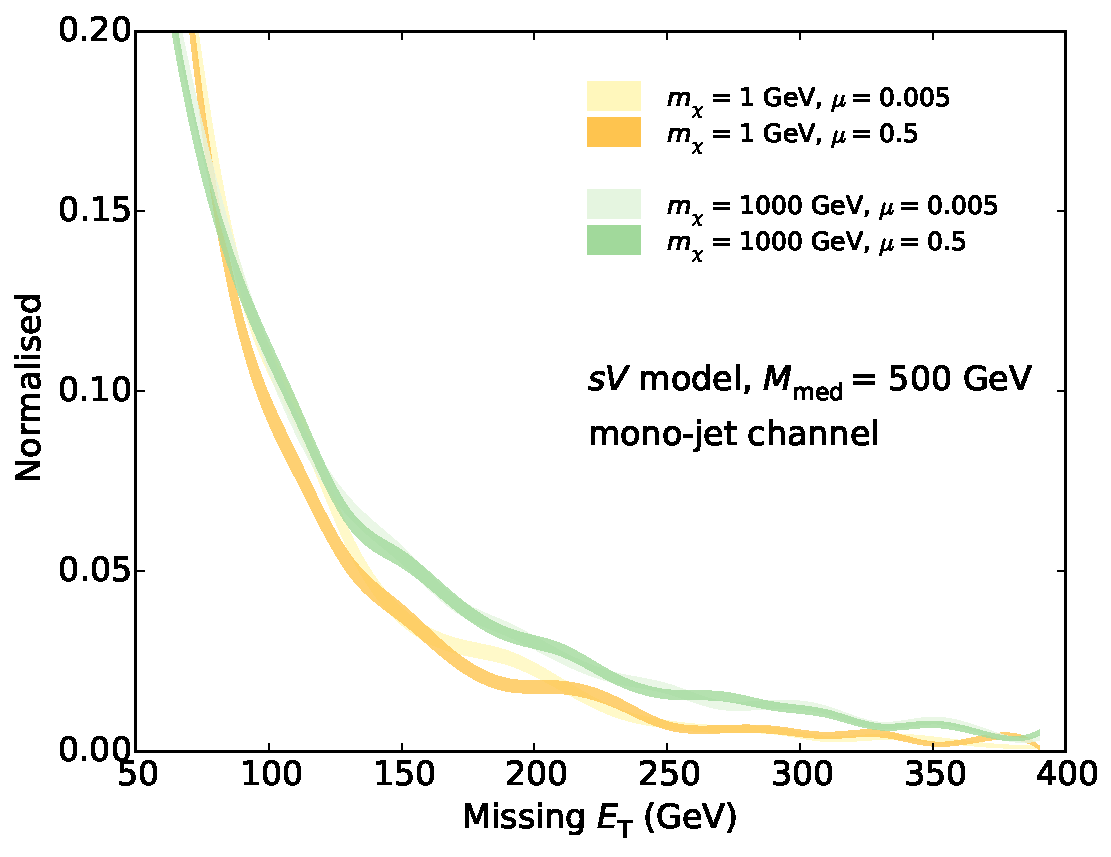
\includegraphics[width=0.495\textwidth]{figures/MET_monojet_SVD.pdf}
    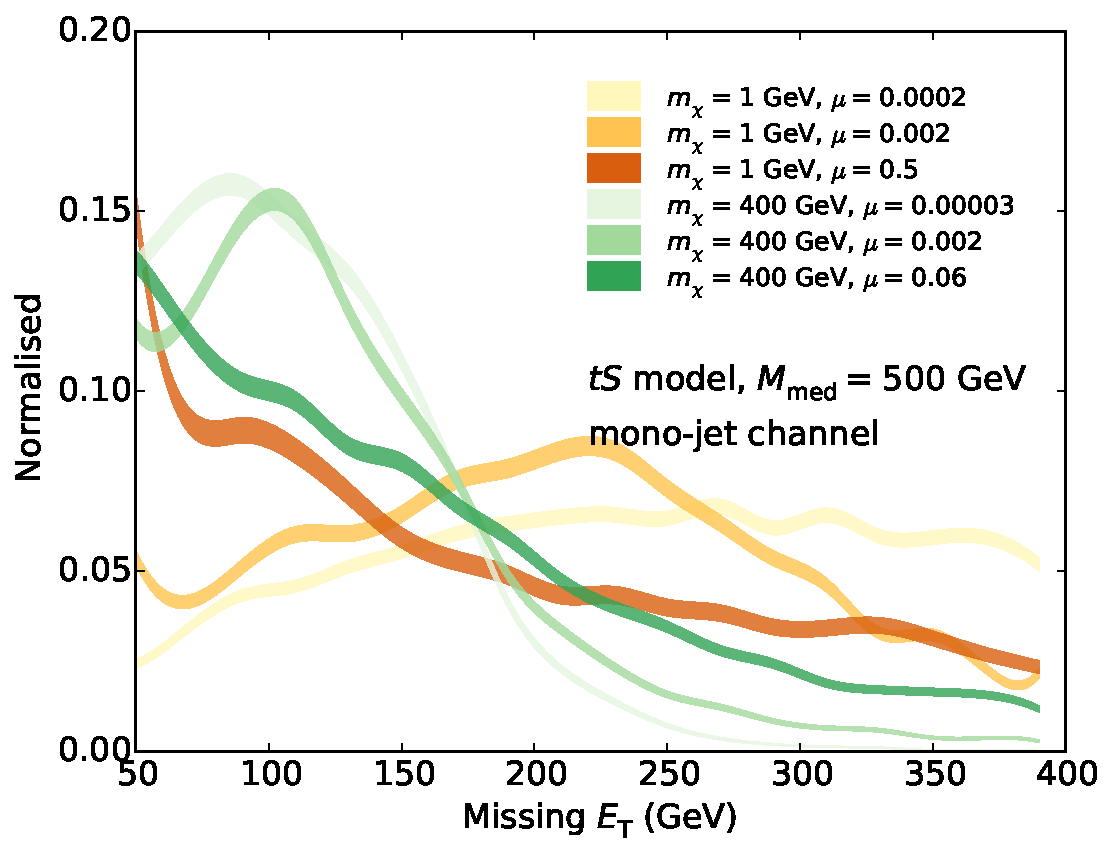
\includegraphics[width=0.495\textwidth]{figures/MET_monojet_TSD.pdf}
    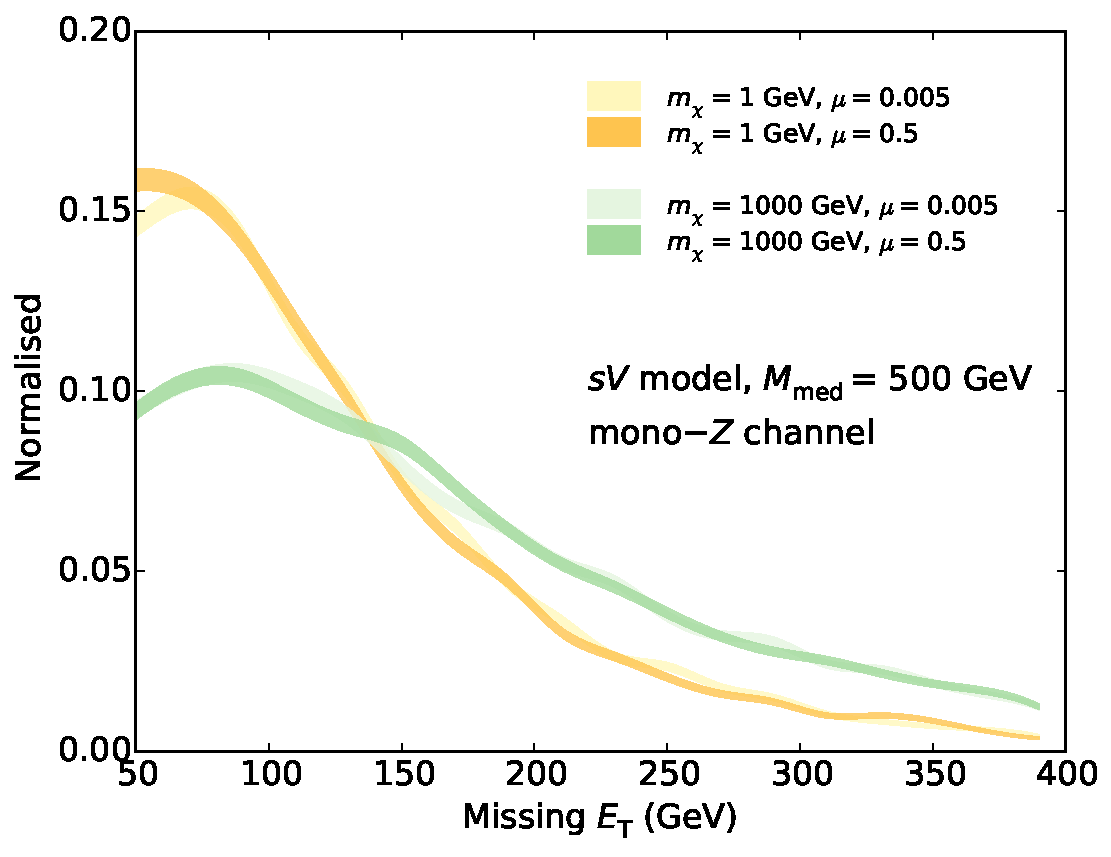
\includegraphics[width=0.495\textwidth]{figures/MET_monoZ_SVD.pdf}
    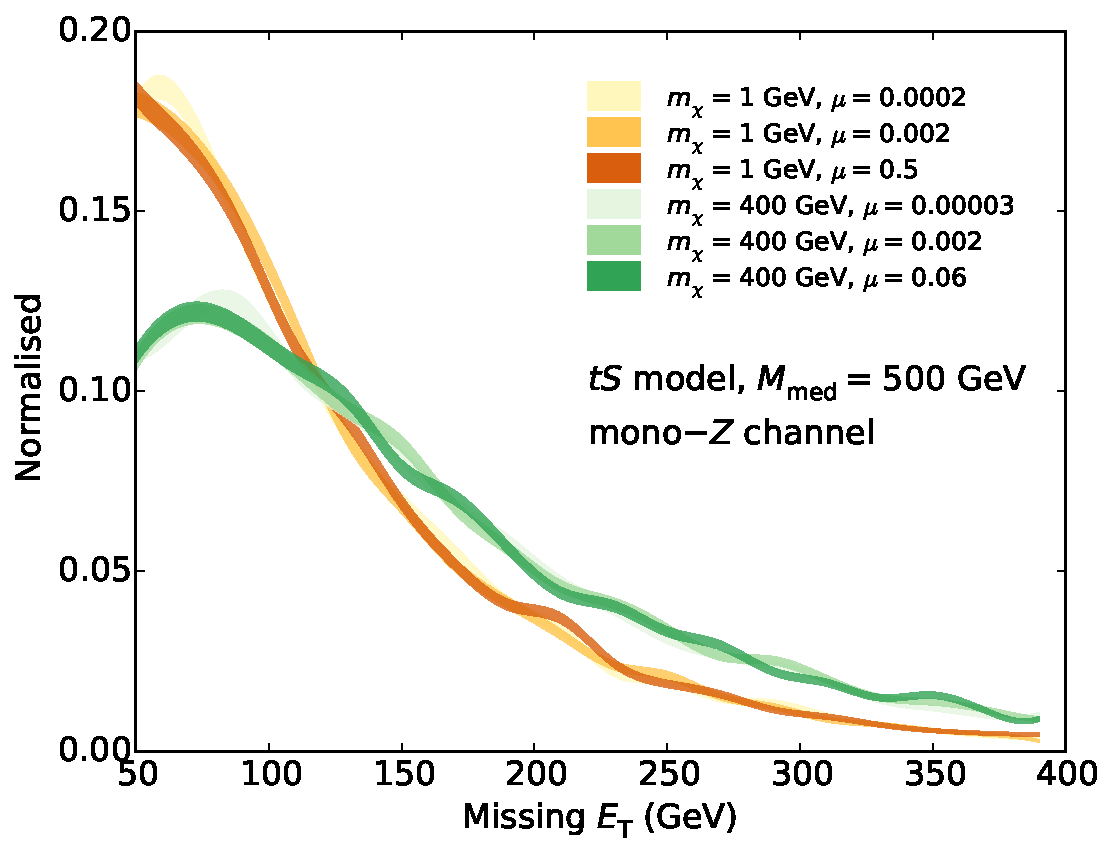
\includegraphics[width=0.495\textwidth]{figures/MET_monoZ_TSD.pdf}
    \caption{The $\met$ distribution of the $sV$ and $tS$ models in the \monojet and \monoZ channels, for some demonstrative masses. The parameter $\mu$ is defined as $\Gamma / \Mmed$, and is used to demonstrate the impact of a changing width; in particular, the $tS$ model in the \monojet channel shows clear width-dependence. The widths are obtained with couplings of 0.1, 1, and 5 where $\mu < 0.5$ remains true.}
    \label{fig:MET_dists}
  \end{center}
\end{figure}

%\textcolor{magenta}{This section should include:}
%\begin{enumerate}
%\item \textcolor{magenta}{Brief motivation for choice of simplified models? (eg. something like "we consider the most straightforward UV-completions of the D1, D5 and D8 effective operators, corresponding to the s-channel scalar, vector and axial-vector models respectively.}
%\item \textcolor{magenta}{The interaction Lagrangians for our four SiMs along with an explanation for why we only assume coupling to SM quarks.}
%\item \textcolor{magenta}{The assumptions and the decay widths associated with our models (?).}
%\item \textcolor{magenta}{Comments on the requirement that $\sqrtgqgX} \leq 4\pi$ in order for the theory to remain perturbative? $\rightarrow$ comments on the choice of mass and coupling points used? Or does this belong in section \ref{sec:sec3}?}
%\end{enumerate}

%Resolving the mediator leads to two possibilities: the mediating particle is exchanged in the s-channel, in which case it may be colour neutral, or it is exchanged in the t-channel in which case it is necessarily coloured \cite{}.

%\cite{ValidEFT, BeyondEFT, CSUSY} t-channel \cite{Buchmueller:2014yoa, SiM}.


\section{Recasting Mono-X Constraints} 
\label{sec:sec3}
The procedure for recasting existing \monoX constraints as simplified model constraints follows a simple cut-and-count methodology. Firstly, signal events are simulated as described in Section \ref{signal_generation}. The event selection criteria of the \monoX analysis of interest is then reproduced and applied to the simulated signal samples. Events surviving the selection criteria are counted to determine both the likelihood of a dark matter event occurring (referred to as the acceptance, $\mathcal{A}$) and the probability of detecting said event (refered to as the efficiency, $\epsilon$). These quantities are then used in combination with channel-specific model-independent limits on new physics events to limit the parameter phase space of a given model.
For a comprehensive description of the recasting procedure, see appendix \ref{Appendix_limitsetting}.
%\bigskip

In this paper, \monojet constraints are derived from a search for new phenomena conducted by the ATLAS Collaboration using $pp$ collisions at $\sqrt{s}=$ 8 TeV as described in Ref. \cite{Aad:2015zva}. Similarly, the leptonic \monoZ and hadronic \monoWZ constraints are derived from ATLAS dark matter searches originally optimised for the D1, D5 and D9 effective operators \cite{Aad:2014monoZlep, ATLASmonoWZ}. These analyses are described in further detail in Sections \ref{monojet_constraints}, \ref{monoZ_constraints} and \ref{monoWZ_constraints} respectively.

%\comm{We should put references to all the papers here! - Amelia}

\subsection{Signal Simulation}
\label{signal_generation}
Signal samples for each channel and for each simplified model were generated as follows. Leading order matrix elements for the process $pp \rightarrow \mathrm{X} + \chi\bar{\chi}$ (where X is specifically one or two jets\footnote{For the \monojet channel, jets are seeded by any parton excluding the (anti-)top quark.}, a $Z(\rightarrow \ell^+ \ell^-)$ boson or a $W/Z(\rightarrow$ jets) boson) were first modelled using \MG$\_${\footnotesize A}MC$@$NLO v2.2.2 \cite{MG_aMCNLO2014} with the MSTW2008lo68cl PDF\cite{MSTW}. During this stage, the renormalisation and factorisation scales were set to the default sum of $\sqrt{m^{2} + p_{T}^{2}}$ for all particles in the final state. Showering and hadronisation were then performed by \PYTHIA  8.201 with the appropriate PDF and using the ATLAS UE Tune AU2-MSTW2008LO~\cite{AUtune}. Reconstruction of small-radius jets for the \monojet channel was performed by FastJet \cite{} using the anti-kT algorithm with a radius parameter, $R$, of 0.4. Similarly, reconstruction of large-radius jets for the \monoWZ channel was performed using the Cambridge-Aachen algorithm with $R$ = 1.2. The latter channel also includes a mass-drop filtering procedure with $\mu$ = 0.67 and $y$ = 0.16 (see ref.~\cite{} for further details). Lastly, the detector response was approximated by applying a Gaussian smearing factor to the $p_{\mathrm{T}}$ of all leptons and jets. 

\subsubsection{Parton Matching Scheme}
\label{matching_procedure}
%\comm{Make explicit the choice of $(0+1+2)j$ vs $(1+2)j$ here.}
%\comm{Also refer to the Papucci paper, and why we don't split the sample. Do we think this is still necessary?}
In the ATLAS \monojet analysis, matching of partons generated in \MG$\mbox{\tiny }$ to jets generated in \PYTHIA is performed using the MLM scheme, with two matching scales, or `QCUTs', per mass/coupling point. The QCUT values span a broad kinematic range in combination with a cut placed on the leading jet $p_{\mathrm{T}}$ per event to avoid double-counting. This treatment aims to mitigate the impact of the matching scale on the shape of the $p_{\mathrm{T}}$ and $\met$ distributions; that is, to reduce the uncertainty in those areas of phase space where the mediator mass is significantly larger or smaller that the QCUT value. For the analysis of simplified models, we use instead a single matching scale of 80 GeV. Though not idyllic, this approach suitably reproduces the results of the ATLAS \monojet analysis for the masses of interest (see Sec. \ref{monojet_validation}). Importantly, it also reduces the complexity and computational expense involved in estimating limits for the \monojet channel.

\bigskip
We now move to a discussion of each of the \monoX channels separately.

\subsection{Mono-jet Constraints}
\label{monojet_constraints}
The ATLAS \monojet + $\met$ \cite{Aad:2015zva} was originally designed to set limits on three new physics scenarios\comm{,}
%\st{: the production of light grativinos in association with gluinos or scalar quarks in a gauge-mediated supersymmetric model, the production of graviton modes in the Arkani-Hamed, Dimopoulos, and Dvali model for large extra spatial dimensions, and}
the most relevant of which is the production of WIMP DM within the context of seven \comm{(?)} effective operators. The analysis also includes a brief study of a $Z'$ DM model which is analogous to our sV model.
%\bigskip

Signal selection is carried out based on at least one hard jet recoiling against missing energy. To ensure that the correct back-to-back jet + $\met$ topology is selected events are required to have a leading jet\footnote{Note: all jets relevant to the ATLAS \monojet and \monoZ analyses are reconstructed with the anti-$k_t$ algorithm with radius parameter 0.4.}, $j_{1}$, with $p_{T} >$ 120 GeV and $|\eta| <$ 2.0 satisfying $p_{T}^{j_{1}}/\met >$ 0.5. Surviving events must then satisfy $|\Delta\phi(j,\metvec)|>1.0$, where $j$ is any jet with $p_{T} >$ 30 GeV and $|\eta| <$ 4.5. This criterion reduces the multijet background contribution where the large $\met$ originates mainly from jet energy mismeasurement. Note that there is no upper limit placed on the number of jets per event. The contribution from the dominant background processes, $W/Z+$jets 
%(\footnote{Do I want to be more specific here? Eg. $W (\rightarrow \ell \nu)+$jets, $Z(\rightarrow \nu\bar{\nu})+$jets, $Z/\gamma^{*}(\rightarrow \ell^{+}\ell^{-})+$jets?})
, is managed with a veto on events containing muons or electrons with $p_{T}>$ 7 GeV. A further veto is placed on events containing isolated tracks\footnote{A track is considered isolated when no additional track with $p_{T} >$ 3 GeV lies within a cone of radius 0.4 around it.} with $p_{T}>$ 10 GeV and $|\eta| <$ 2.5. This reduces the contribution from non-identified leptons ($e$, $\mu$ or $\tau$) in the final state. Lastly, nine separate signal regions are defined with increasing lower thresholds on $\met$, which range from 150 GeV to 700 GeV as shown in Table \ref{monojet_SRs}.
%\st{initially, events are required to have $\met>$ 150 GeV and at least one jet with $p_{T} >$ 30 GeV and $|\eta| <$ 4.5} (\comm{My logic here is that these cuts are for trigger, or pre-selection - they are overwritten by later cuts, right? So I think not worth including.}). we require $|\Delta\phi(\mathrm{j},\metvec)|>1.0$, where j is any jet with $p_{T} >$ 30 GeV and $|\eta| <$ 4.5.  have a leading jet (\comm{Is this the dominant background? If so, include `dominant', if not, this cut is maybe better understood as implementing back-to-backness. Is there an upper limit on $N_{jets}$?}). \comm{Note to self: include lepton veto criteria here.}
%\bigskip

The ATLAS \monojet analysis revealed no significant deviation of observed events from the expected SM backgrounds in the Run 1 8 TeV dataset. Subsequently, limits on new physics signatures were derived in terms of the visible cross-section, $\sigma\times\mathcal{A}\times\epsilon$, using the HistFitter package \cite{}. These model-independent limits are shown in Table \ref{monojet_SRs} and correspond to the 95\% confidence level.

\begin{table}[!htbp]
\centering
\begin{tabular}{c|c|c}
 \hline
 \hline
 Signal Region & $\met$ threshold [GeV] & $\sigma \times \mathcal{A} \times \epsilon$ [fb] \\ %$N_{obs}$ & $N_{exp}$ \\%& $N_{obs}/\mathcal{L}$ & $N_{exp}/\mathcal{L}$ \\
 \hline
 SR1 & 150 & 726 (935) \\ %14737.8 & 18980.5 \\%726 & 935 \\
 SR2 & 200 & 194 (271) \\ %3938.2 & 5501.3 \\%194 & 271 \\
 SR3 & 250 & 90 (106) \\ %1827 & 2151.8 \\%90 & 106 \\
 SR4 & 300 & 45 (51) \\ %913.5 & 1035.3 \\%45 & 51 \\
 SR5 & 350 & 21 (29) \\ %426.3 & 588.7 \\%21 & 29 \\
 SR6 & 400 & 12 (17) \\ %243.6 & 345.1 \\%12 & 17 \\
 SR7 & 500 & 7.2 (7.2) \\ %146.16 & 146.16 \\%7.2 & 7.2 \\
 SR8 & 600 & 3.8 (3.2) \\ %77.14 & 73.08 \\%3.8 & 3.6 \\
 SR9 & 700 & 3.4 (1.8) \\ %69.02 & 36.54 \\%3.4 & 1.8 \\
 \hline
 \hline
\end{tabular}
\caption{The ATLAS \monojet $\met$ signal regions and corresponding observed (expected) model-independent upper limits on $\sigma \times \mathcal{A} \times \epsilon$ at 95\% confidence level. Adapted from Ref. \cite{Aad:2015zva}.
%The ATLAS model-independent upper limits on the number of observed (expected) signal events, $N_{obs}$ ($N_{exp}$), at 95\% confidence level for the \monojet channel signal regions.
%\comm{Since this table is adapted from the \monojet paper, I think we should reproduce exactly what they show, ie the limit on $\sigma \times \mathcal{A} \times \epsilon$. Part of the reason is that if you multiply their values by the lumi, this is ignoring the uncertainty on that lumi that they've already included. More importantly, I don't think there is any advantage in showing the limits on $N$, since to obtain limits on $\sigma$ we divide immediately by $\mathcal{L}$ again anyway, plus the audience may be more familiar with the limit on $\sigma \times \mathcal{A} \times \epsilon$.}
}
\label{monojet_SRs}
\end{table}

The signal simulation procedure outlined in sec. \ref{signal_generation} and implementation of the selection criteria discussed above were validated for the \monojet channel via reproduction of ATLAS limits on the suppression scale, $\Mstar \equiv \Mmed / \sqrtgqgX$, for the $Z'$ model. The details of this process are contained in appendix \ref{monojet_validation}. Importantly, we observe agreement within $\sim$12\% for all samples.

%\st{Note that we only calculate limits on M$_{*}$ for this aspect of the analysis. Although it is customary to present constraints on dark matter models in the form of limits on M$_{*}$, we shall hereafter present constraints in the form of limits on the cross-section. This is done to better facilitate the comparison of collider and direct detection results, where $\sigma(pp \rightarrow X + \chi\bar{\chi})$ and $\sigma(N\chi \rightarrow N\chi)$ are related by a Fierz transformation in the simplified model framework} \cite{PJFox, NBellDent}.

%\draft{While the signal samples used by the ATLAS group (and for validation) correspond to the processes $pp \rightarrow j\chi\bar{\chi}$ and $pp \rightarrow jj\chi\bar{\chi}$ where $j$ is a final state jet, \monojet constraints on the simplified models studied in this paper were set using signal samples with zero, one and two jets in the final state.} \comm{This deviation from the ATLAS analysis is motivated by the observation that the limits on $\Mstar$ are improved with the addition of the process $pp \rightarrow \chi\bar{\chi}$.}
%However, while the ATLAS MC samples are generated for only two matching scale values (80 GeV and 300 GeV), we use a sliding value of $\mX/4$. \comm{This ensures that all jet-related kinematic distributions are smoothly connected across all dark matter masspoints.}

\subsection{Mono-$Z$ Constraints}
\label{monoZ_constraints}
The ATLAS mono-$Z(\rightarrow \ell^+ \ell^-)$ + $\met$ analysis \cite{Aad:2014monoZlep} was principally designed to constrain a set of EFT models of DM. As a secondary focus, it also includes a short study of a $t$-channel simplified model similar to our tS model.
%\textcolor{blue}{This model is used to validate our results in this channel; see the details in sec.~\ref{monoZ_validation}.} \comm{Can this go at the end of this subsection?}

The selection criteria for this analysis are summarised as follows (see the paper for a full description). Electrons (muons) are required to have a $p_{\mathrm{T}}$ greater than 20 GeV, and $|\eta|$ less than 2.47 (2.5). Two opposite-sign, same-flavour leptons are selected, and required to have invariant mass and pseudorapidity such that $m_{\ell \ell} \in [76, 106]$ GeV and $|\eta^{\ell \ell}| < 2.5$. The reconstructed $Z$ boson should be approximately back-to-back and balanced against the $\met$, ensured with the selections $\Delta \phi (\metvec, p_{\mathrm{T}}^{\ell \ell}) > 2.5$ and $| p_{\mathrm{T}}^{\ell \ell} - \met | \, /  \, p_{\mathrm{T}}^{\ell \ell} < 0.5$. Events containing a jet with $p_{\mathrm{T}}>$ 25 GeV and $|\eta|< $ 2.5 are vetoed. Events are also vetoed if they contain a third lepton with $p_{\mathrm{T}}>$ 7 GeV. The signal regions are defined by increasing lower $\met$ thresholds: $\met >$ 150, 250, 350, 450 GeV.

% Note: I haven't included any info on the overlap removal here.

%The dominant background in this analysis is the irreducible $ZZ \rightarrow \ell^+ \ell^- \bar{\nu} \nu$ process, which has a softer $\met$ distribution that the DM signal. The background is estimated with MC simulation, and has a systematic uncertainty in the range 36-46$\%$ across the four signal regions.

A cut-and-count strategy is used to estimate the total observed yields and expected SM backgrounds in each signal region. The statistical, systematic, and luminosity uncertainties are added in quadrature to give the total background estimate and uncertainty. We convert these into model-independent upper limits on the expected (observed) number of new physics events, $N^{\mathrm{exp}}_{\mathrm{sig}}$ ($N^{\mathrm{obs}}_{\mathrm{sig}}$), with a simple implementation of HistFitter that uses a frequentist calculator and a one-sided profile likelihood test statistic (the LHC default). The results of this process are presented in Table \ref{tab:Nlim_monoZ}. Note that we use signal regions 1 and 2 only, as our simplified HistFitter approach is inadequate to handle the very low statistics of signal regions 3 and 4. These upper limits are also used for the validation of the \monoZ signal generation and selection procedures (see sec.~\ref{monoZ_validation}).

\begin{table}
\begin{center}
\begin{tabular}{ c  c  c }
\hline
\hline
& SR1 & SR2 \T \\
& ($E_{\mathrm{T}}^{\mathrm{miss}} > $ 150 GeV) & ($E_{\mathrm{T}}^{\mathrm{miss}} > $ 250 GeV) \B \\
\hline
$N_{\mathrm{sig}}^{\mathrm{exp}}$ & 34.7 & 6.8 \T \\
$N_{\mathrm{sig}}^{\mathrm{obs}}$ & 32.2 & 5.9 \B \\
\hline
\hline
\end{tabular}
\end{center}
\label{tab:Nlim_monoZ}
\caption{The expected and observed upper limits on the number of new physics events in the ATLAS \monoZ analysis, calculated with HistFitter using the results of \cite{Aad:2014monoZlep}.}
\end{table}

\subsection{Mono-$W/Z$ Constraints}
\label{monoWZ_constraints}

The analysis focusing on fully-hadronic decays of the bosons in the \monoWZ channel performed by ATLAS on the 8 TeV dataset was considered especially interesting, since constructive interference in the mono-$W(\rightarrow \ell \nu)$ channel was assumed to be possible for the vector EFT operator, leading to stronger limits than those from the \monojet searches in this case. More recently however, studies have revealed that such a scenario would violate unitarity and this interpretation is not emphasised in this work due to these concerns.

Nevertheless, this channel is an interesting addition, since it exploits the large branching fraction of hadronic boson decays. Also, the experimental techniques applied are significantly different; the selection is based on large-$R$ jets that are consistent with having come from an electroweak boson. In addition, large $\met$ is required, as for all \monoX searches.

The applied event selection is summarised in the following. Large-radius jets are reconstructed with the Cambridge-Aachen algorithm using radius parameter $R = 1.2$. A mass drop filter \ref{} is applied, where $\sqrt{y}>0.4$\footnote{$\sqrt{y} = \mathrm{min}(p_{\mathrm{T}_{j1}},p_{\mathrm{T}_{j2}})\Delta R / m_{jet}$, i.e. the momentum balance of the two leading subjets.} is required in order to suppress non-$W/Z$ processes.
Events with at least one large-radius jet with $p_{\mathrm{T}} >$ 250 GeV, $|\eta| <$ 1.2 and a mass within a window around the $W/Z$ mass, between 50 and 120 GeV, are selected.
To reduce the $t \bar{t}$ and QCD backgrounds, events containing small-$R$ (replace with `narrow' here?) jets (reconstructed with the anti-$k_T$ algorithm and radius parameter $R$ = 0.4) with $\Delta\phi(\mathrm{jet},\met)< 0.4$ or more than one jet ($p_{\mathrm{T}} >$ 40 GeV, $|\eta| <$ 4.5) with $\Delta R$(jet, large-$R$ jet)$>0.9$, are vetoed. Electrons, muons and photons are vetoed if their $p_{\mathrm{T}}$ is larger than 10 GeV and they are within $|\eta| <$ 2.47 (electrons), 2.5 (muons), 2.37 (photons). The original analysis considers two signal regions: $\met > 250$ GeV and $\met > 500$ GeV. We consider in the following only the signal region with $\met > 500$ GeV (\comm{should have a statement explaining this choice}).

The main background is due to $Z \rightarrow \bar{\nu} \nu$ events with additional jets from initial state radiation. Further important backgrounds from $W/Z$+jets events, in which the boson decays leptonically, enter the selection if the lepton(s) is missed due to being out of the acceptance range or failing ID requirements, or in the case that it is a hadronically-decaying $\tau$ lepton. All these backgrounds are estimated by the original analysis in dedicated control regions.

Whereas the ATLAS analysis uses a shape fit of the mass distribution of the large-radius jet, we simply regard the number of events in the signal region, since the data points of the $m_{\rm jet}$ distribution were not published. \comm{check!!!} From the published number of expected and observed events in the signal region and their uncertainties, we \comm{use HistFitter to} calculate the upper limit on the number of new physics events as described above for the \monoZ channel (see eq.~\ref{sigma_nom}). We obtain the following numbers:  $N_{exp} = 27.2$, $N_{obs} = 27.4$.


\section{Limits on $\sigma(pp \rightarrow X + \chi\bar{\chi})$ and $\sqrt{g_{q}g_{\chi}}$} 
\label{sec:sec4}
%\begin{flushleft}
The 95\% confidence level upper limits on the observed cross-section for the process $pp \rightarrow X\chi\bar{\chi}$ (where $X$ is either 0, 1 or 2 jets or a Z boson) are presented here for each simplified model. Also shown are the 95\% CL upper limits on the coupling strengths between the dark and Standard Model sectors, denoted collectively by the variable $\sqrt{g_{q}g_{\chi}}$. These quantities are evaluated as described in appendix \ref{AppendixB} and correspond to the best limits.
\bigskip

\textcolor{magenta}{This section should include:}
\begin{enumerate}
\item \textcolor{magenta}{Plots for $\sigma(pp \rightarrow X \chi \bar{\chi}$ as a function of $m_{\chi}$ for fixed $m_{M}$ and $f$ along with the limits on $f$ using $\sigma \sim f^{4}$.}
\item \textcolor{magenta}{Brief interpretation of the results. I.e. explain "in words" what the plots illustrate.}
\item \textcolor{magenta}{Comparison with previous results (?).}
\end{enumerate}
\end{flushleft}

\subsection{Mono-jet channel}
\comm{Just a note here to remind me - it would be nice to have a plot here demonstrating the effect of the width on the kinematics (MET in particular) for the $t$-channel model, and maybe the $s$-channel model if we get the coupling strength low enough. - Amelia}

\begin{figure}[!h]
\begin{center}
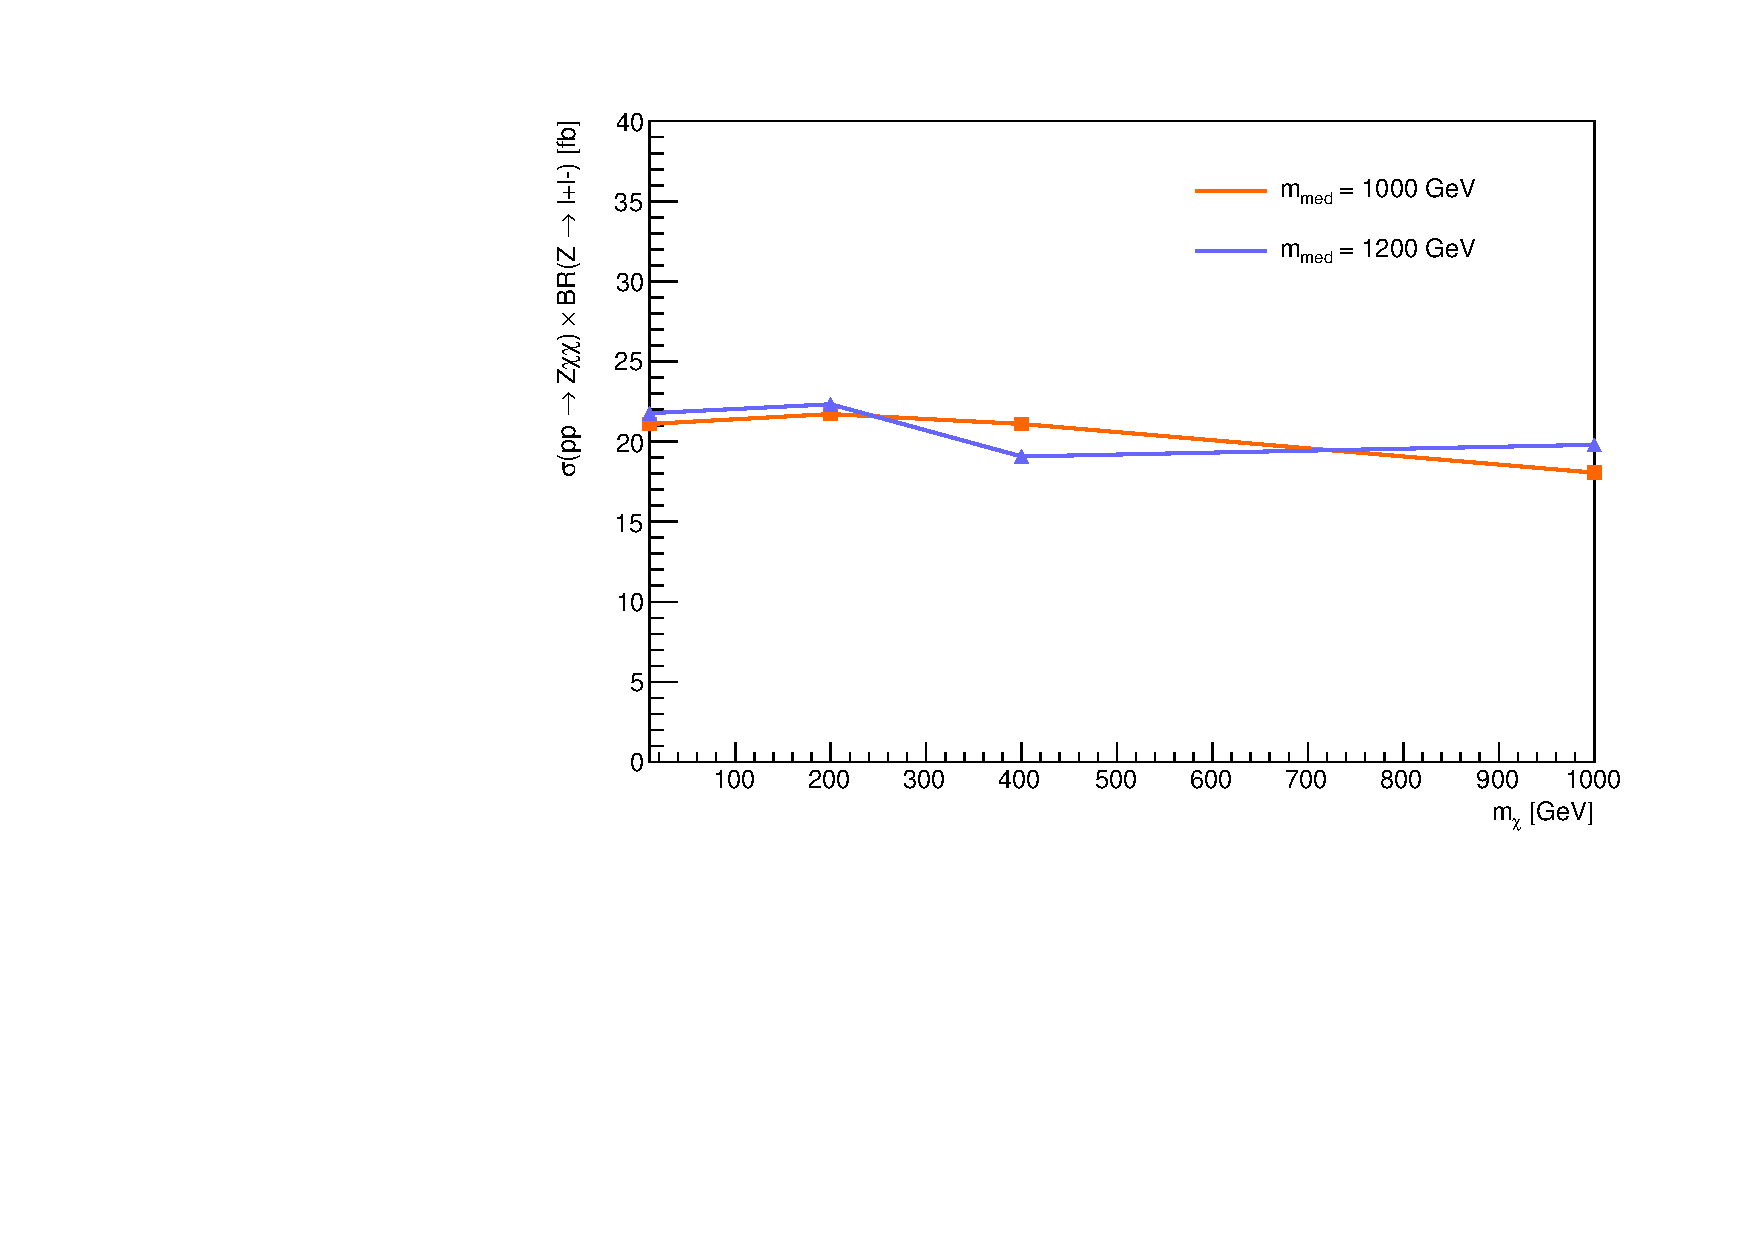
\includegraphics[width=0.45\textwidth]{figures/monoZ_sigma_limits_variedDMmass.pdf}
\caption{A very rough first plot - to be prettified! Shows the limit on sigma x BR for the sV model in the mono-Z (should be mono-jet) channel. Will change to have a band for the expected limit, and a line for the observed limit. Show 5 different coupling scenarios on one plot. Mono-Z (jet) channel, sV model.}
\label{fig:MonoZ_SVD_limit}
\end{center}
\end{figure}

\begin{figure}[!h]
\begin{center}
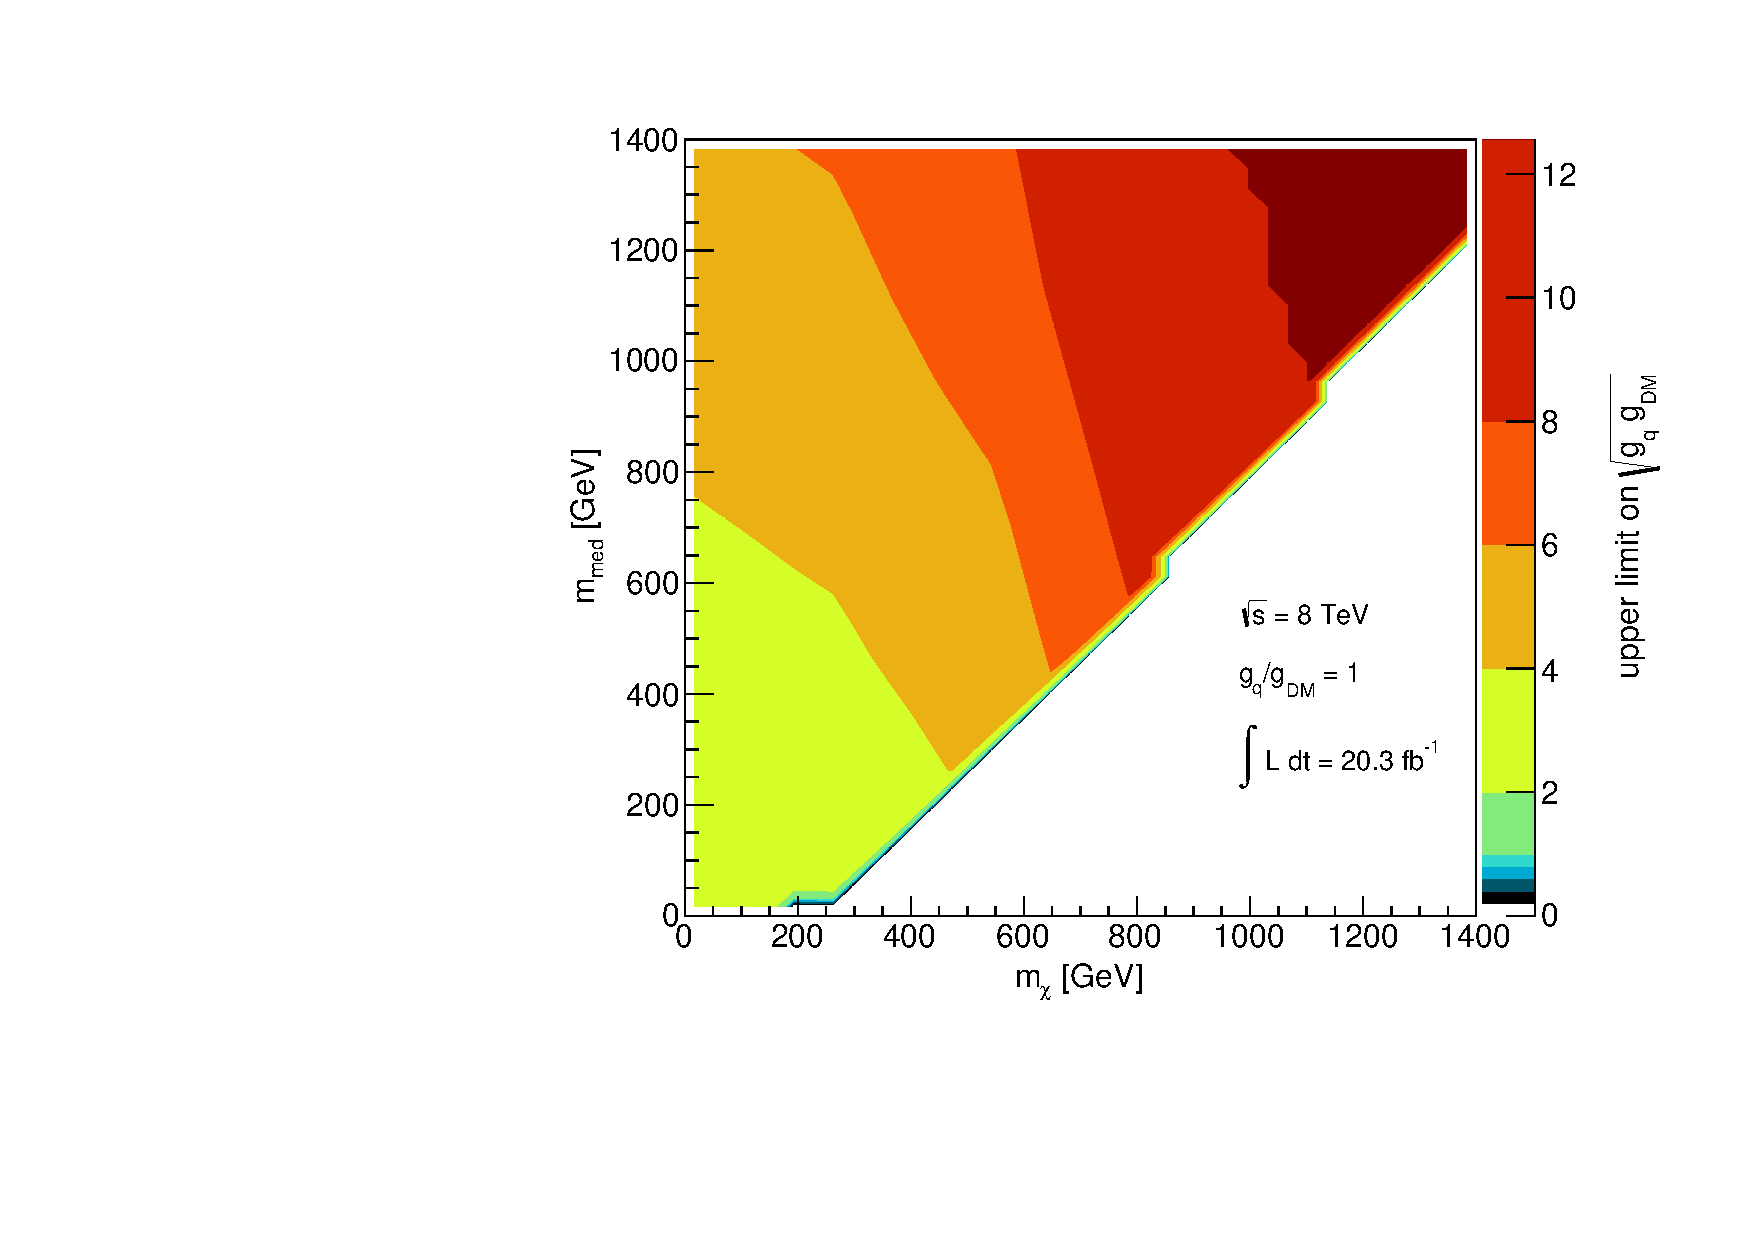
\includegraphics[width=0.45\textwidth]{figures/coupling_limits_TSD_1.pdf}
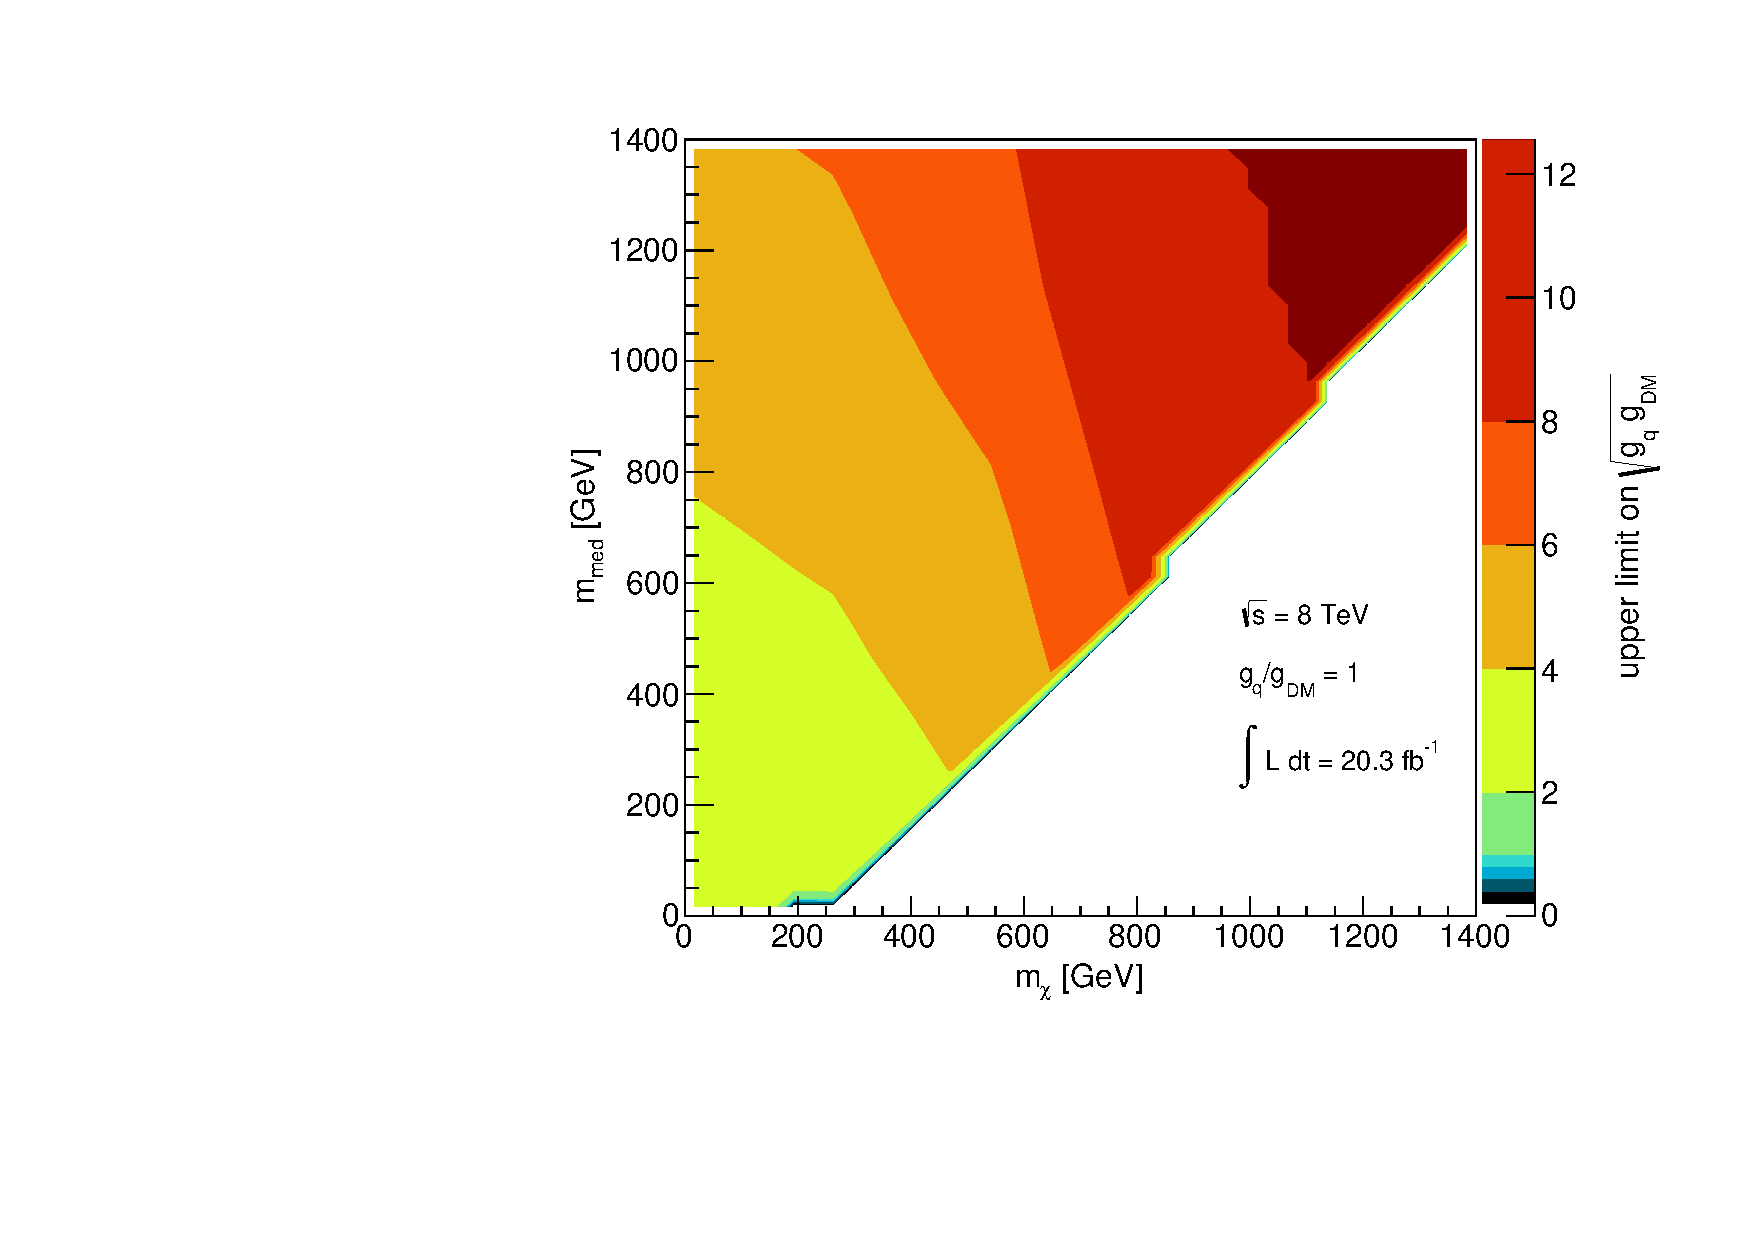
\includegraphics[width=0.45\textwidth]{figures/coupling_limits_TSD_1.pdf}
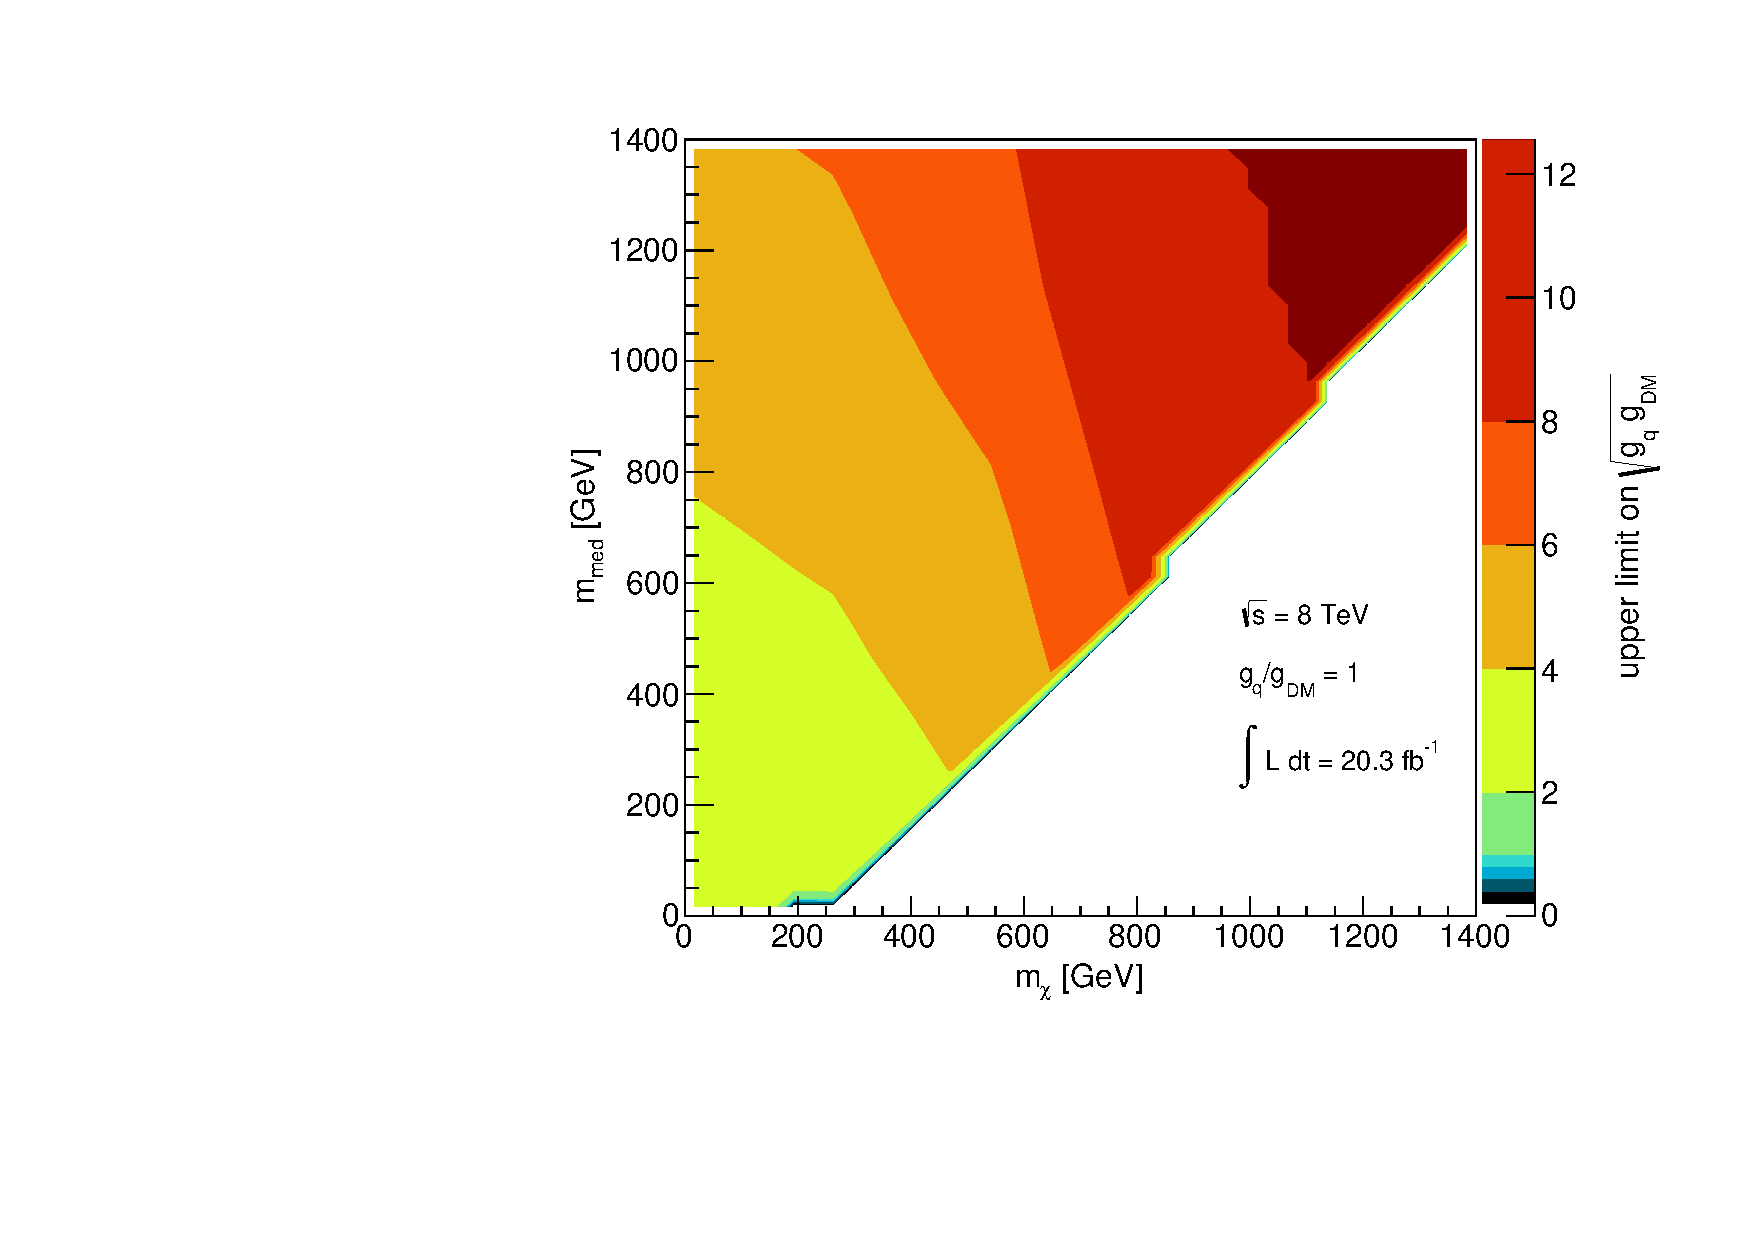
\includegraphics[width=0.45\textwidth]{figures/coupling_limits_TSD_1.pdf}
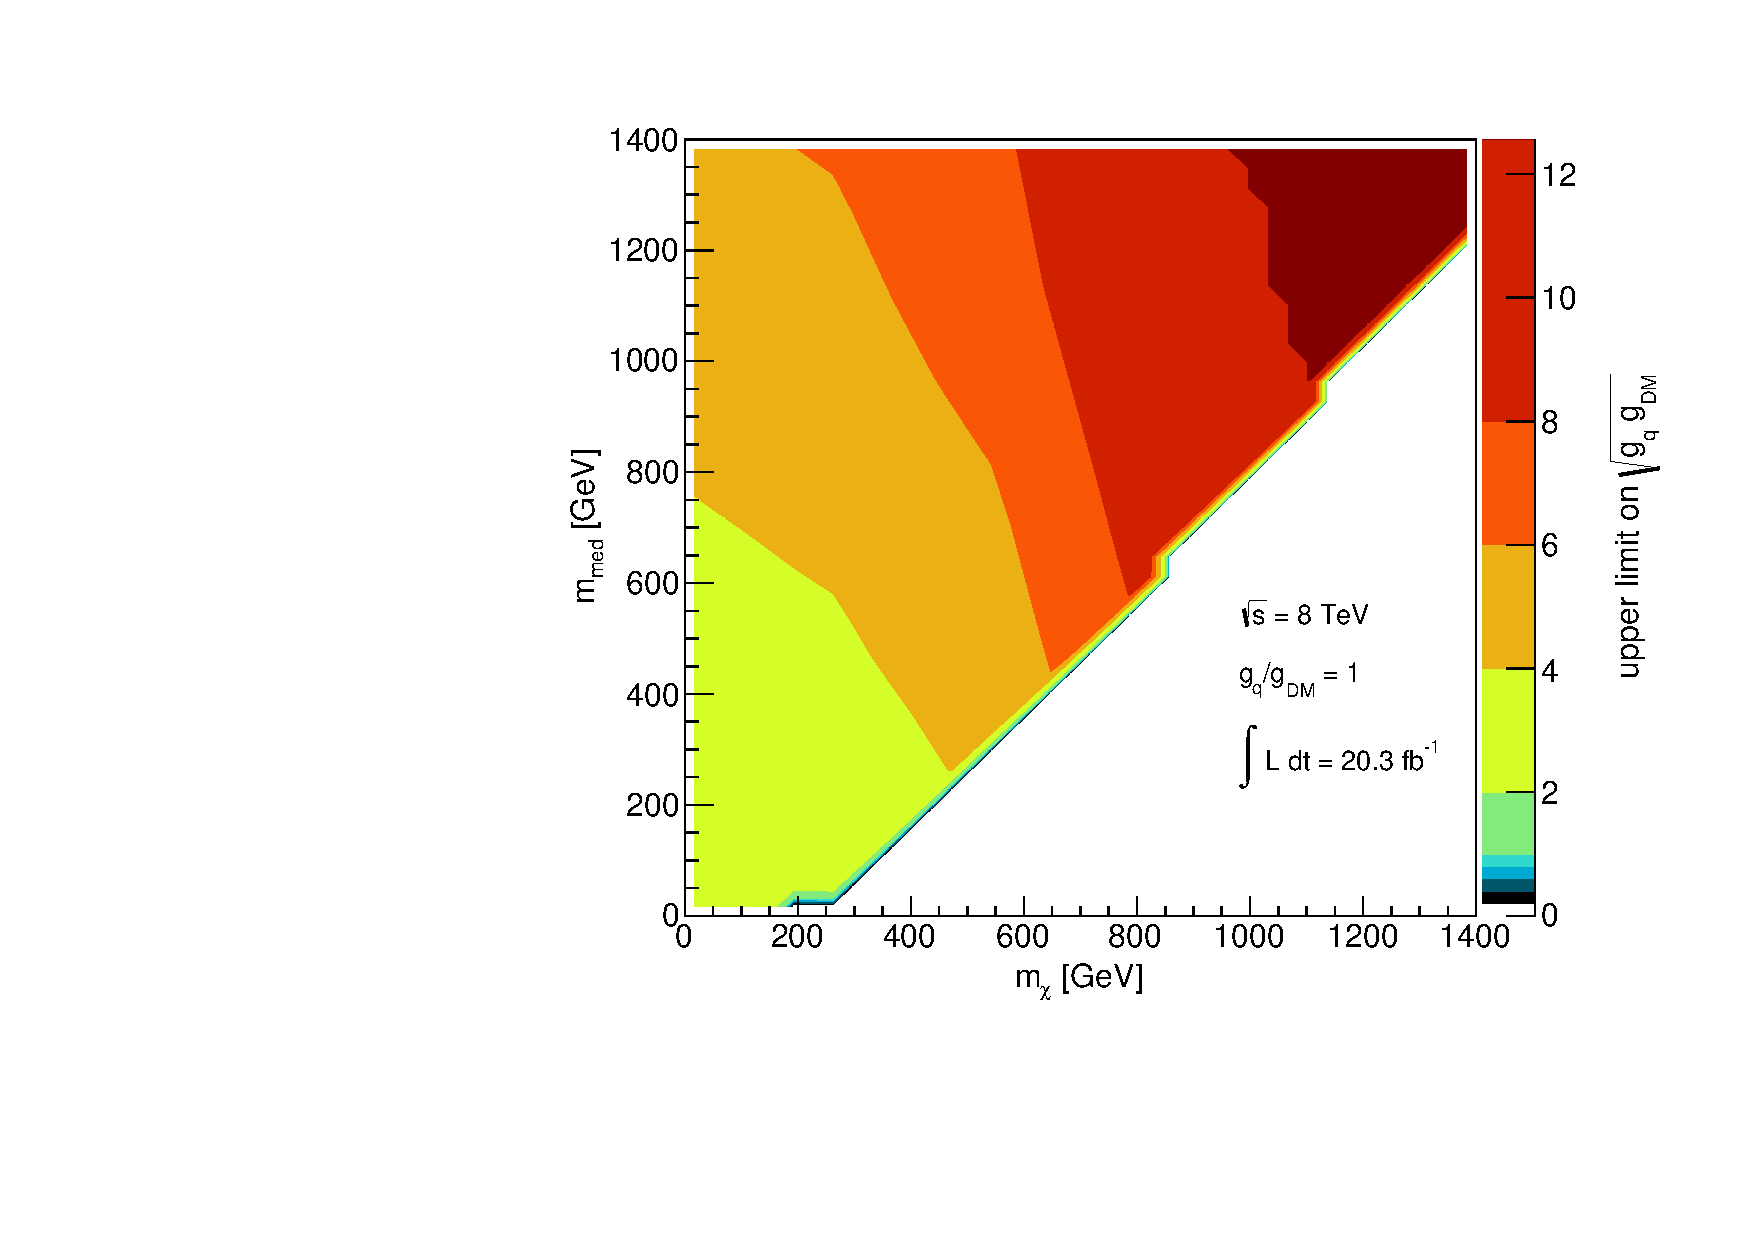
\includegraphics[width=0.45\textwidth]{figures/coupling_limits_TSD_1.pdf}
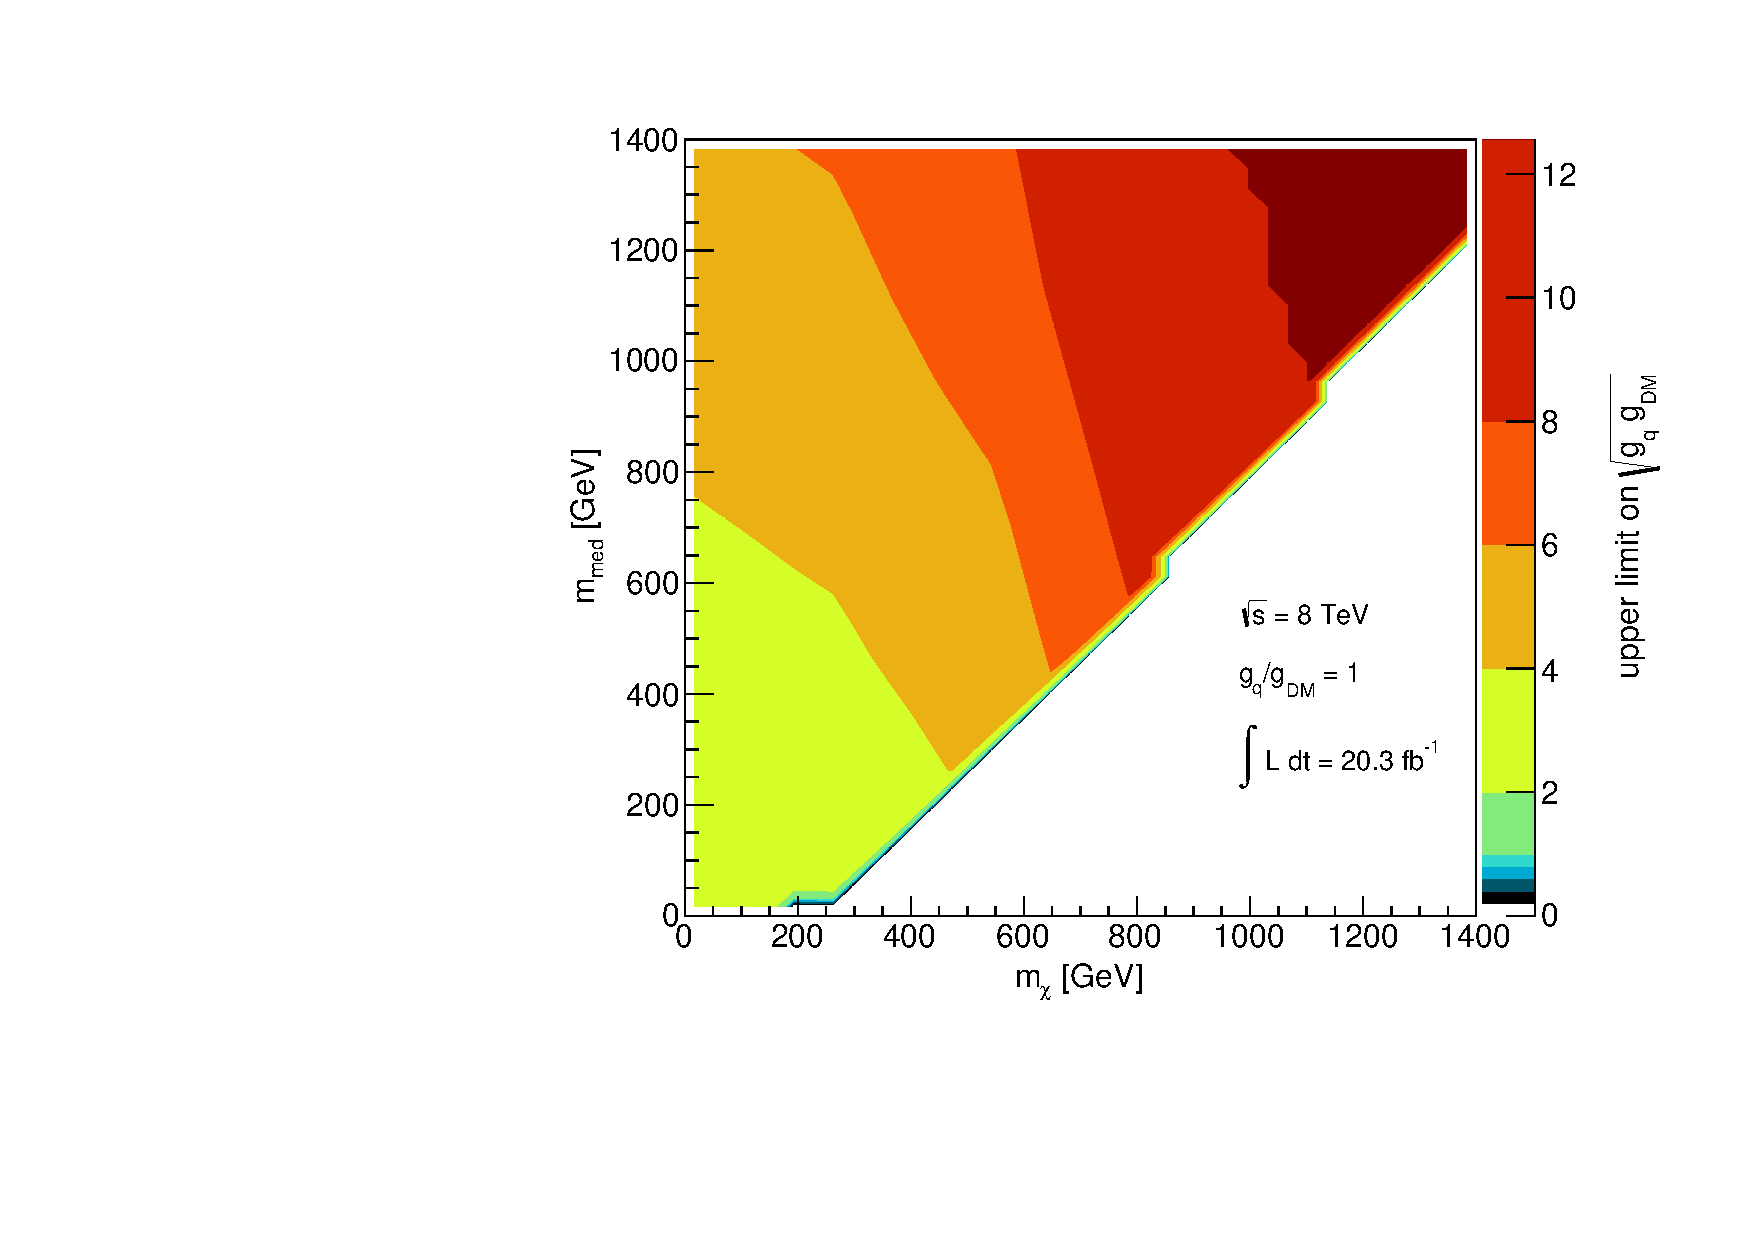
\includegraphics[width=0.45\textwidth]{figures/coupling_limits_TSD_1.pdf}
\caption{Limit on coupling strength for the sV model, in the mono-Z (should be jet) channel.  Need to fix up the scale on the z-axis and include mass points as dots on the plot. To be replaced with 5 plots with different coupling ratios, gq/gchi = 0.2, 0.5, 1, 2, 5. REPLACE WITH SV MODEL PLOTS.}
\label{fig:Monojet_SVD_couplinglimit}
\end{center}
\end{figure}

\begin{figure}[!h]
\begin{center}
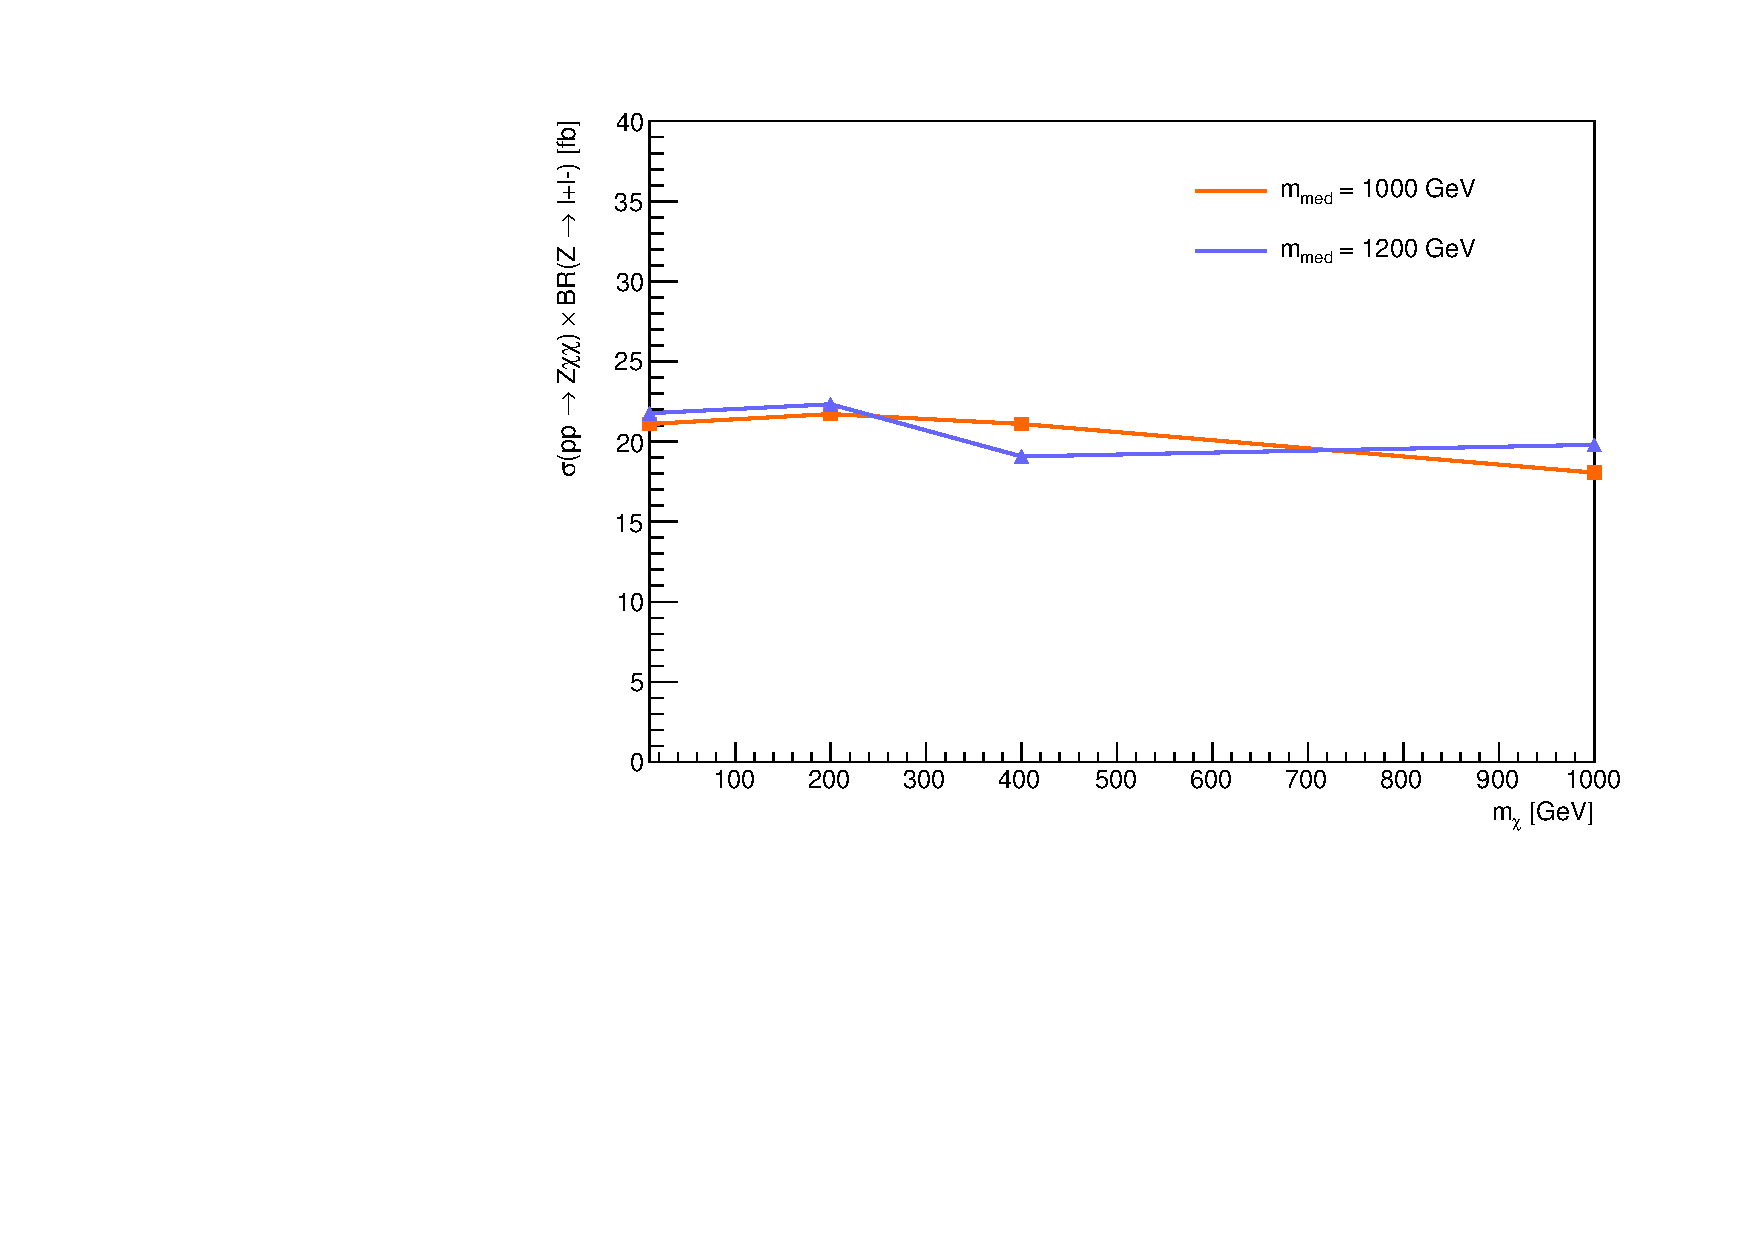
\includegraphics[width=0.45\textwidth]{figures/monoZ_sigma_limits_variedDMmass.pdf}
\caption{Mono-jet channel, sS model. REPLACE WITH SS MODEL PLOTS.}
\label{fig:Monojet_SSD_limit}
\end{center}
\end{figure}

\begin{figure}[!h]
\begin{center}
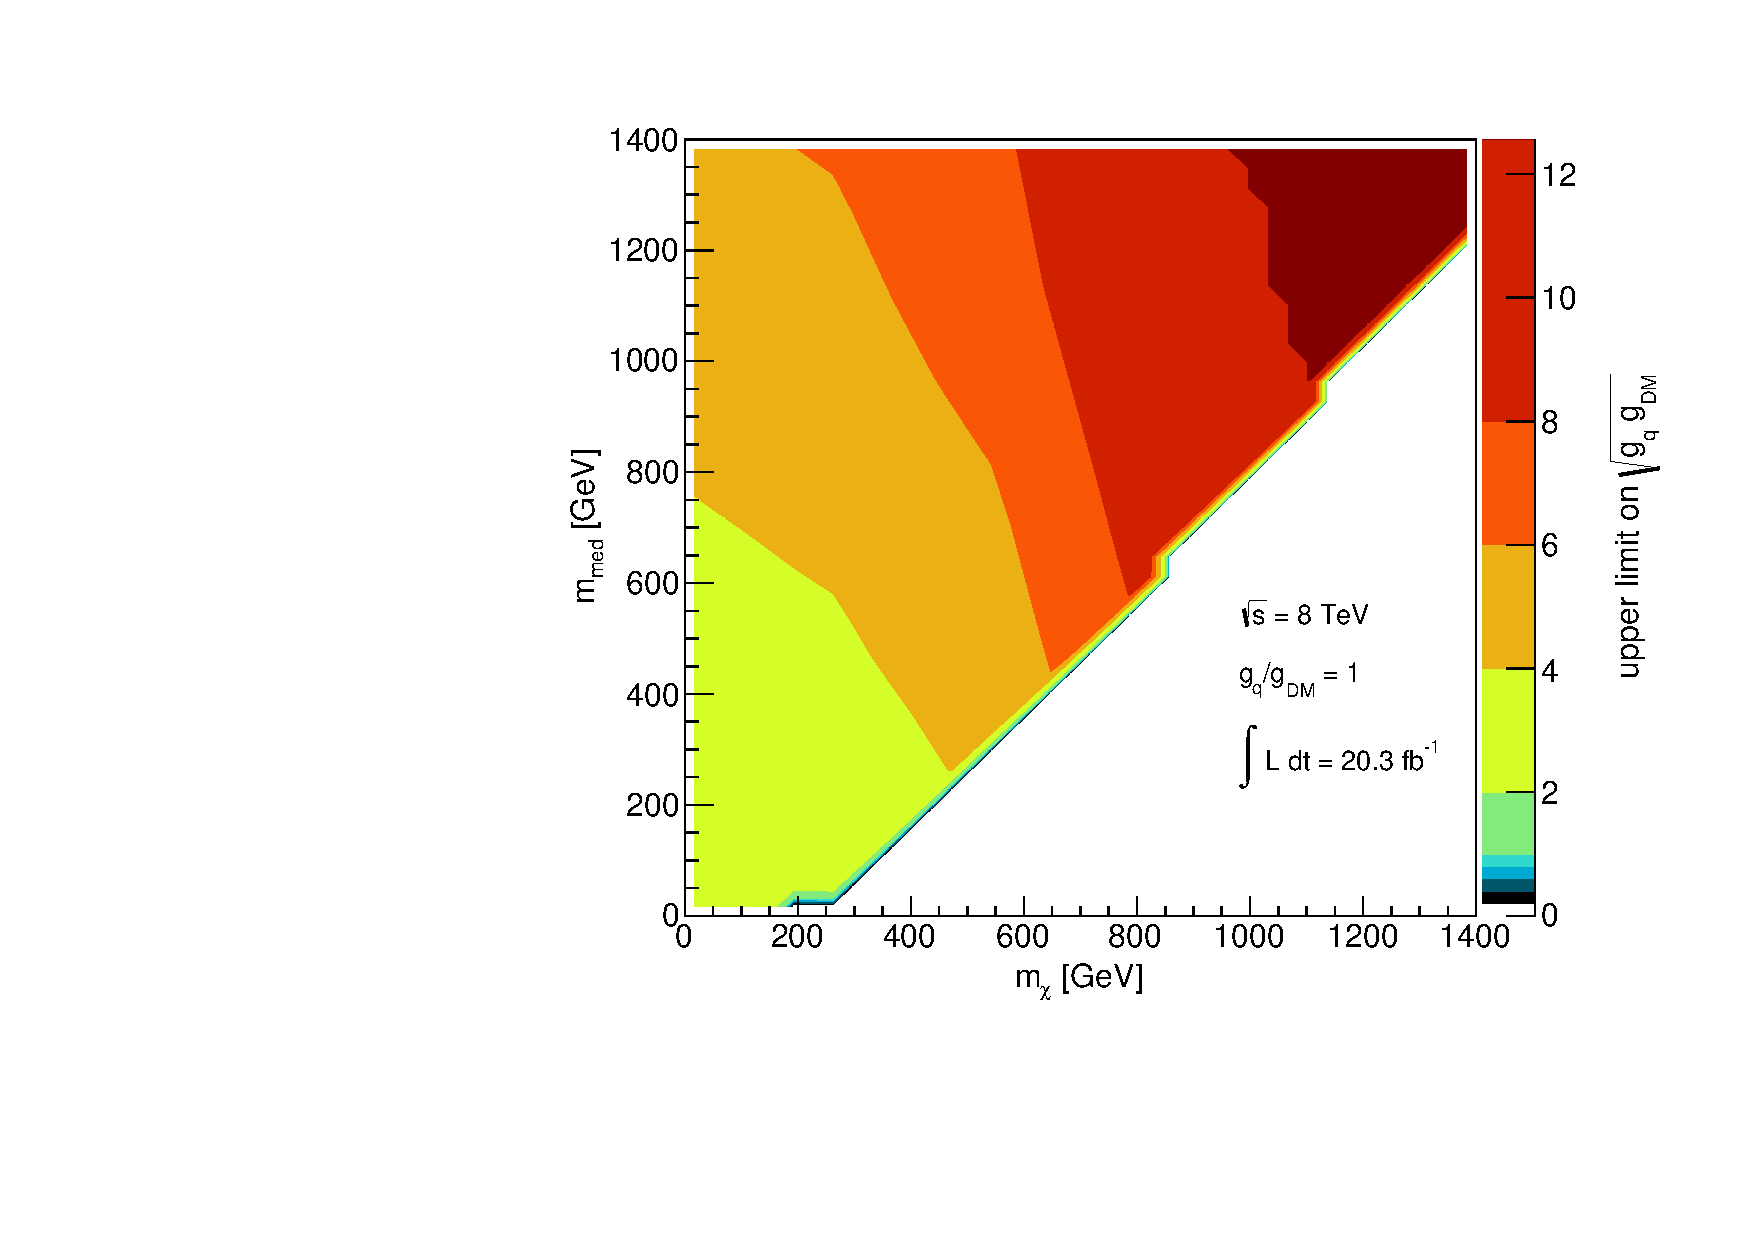
\includegraphics[width=0.45\textwidth]{figures/coupling_limits_TSD_1.pdf}
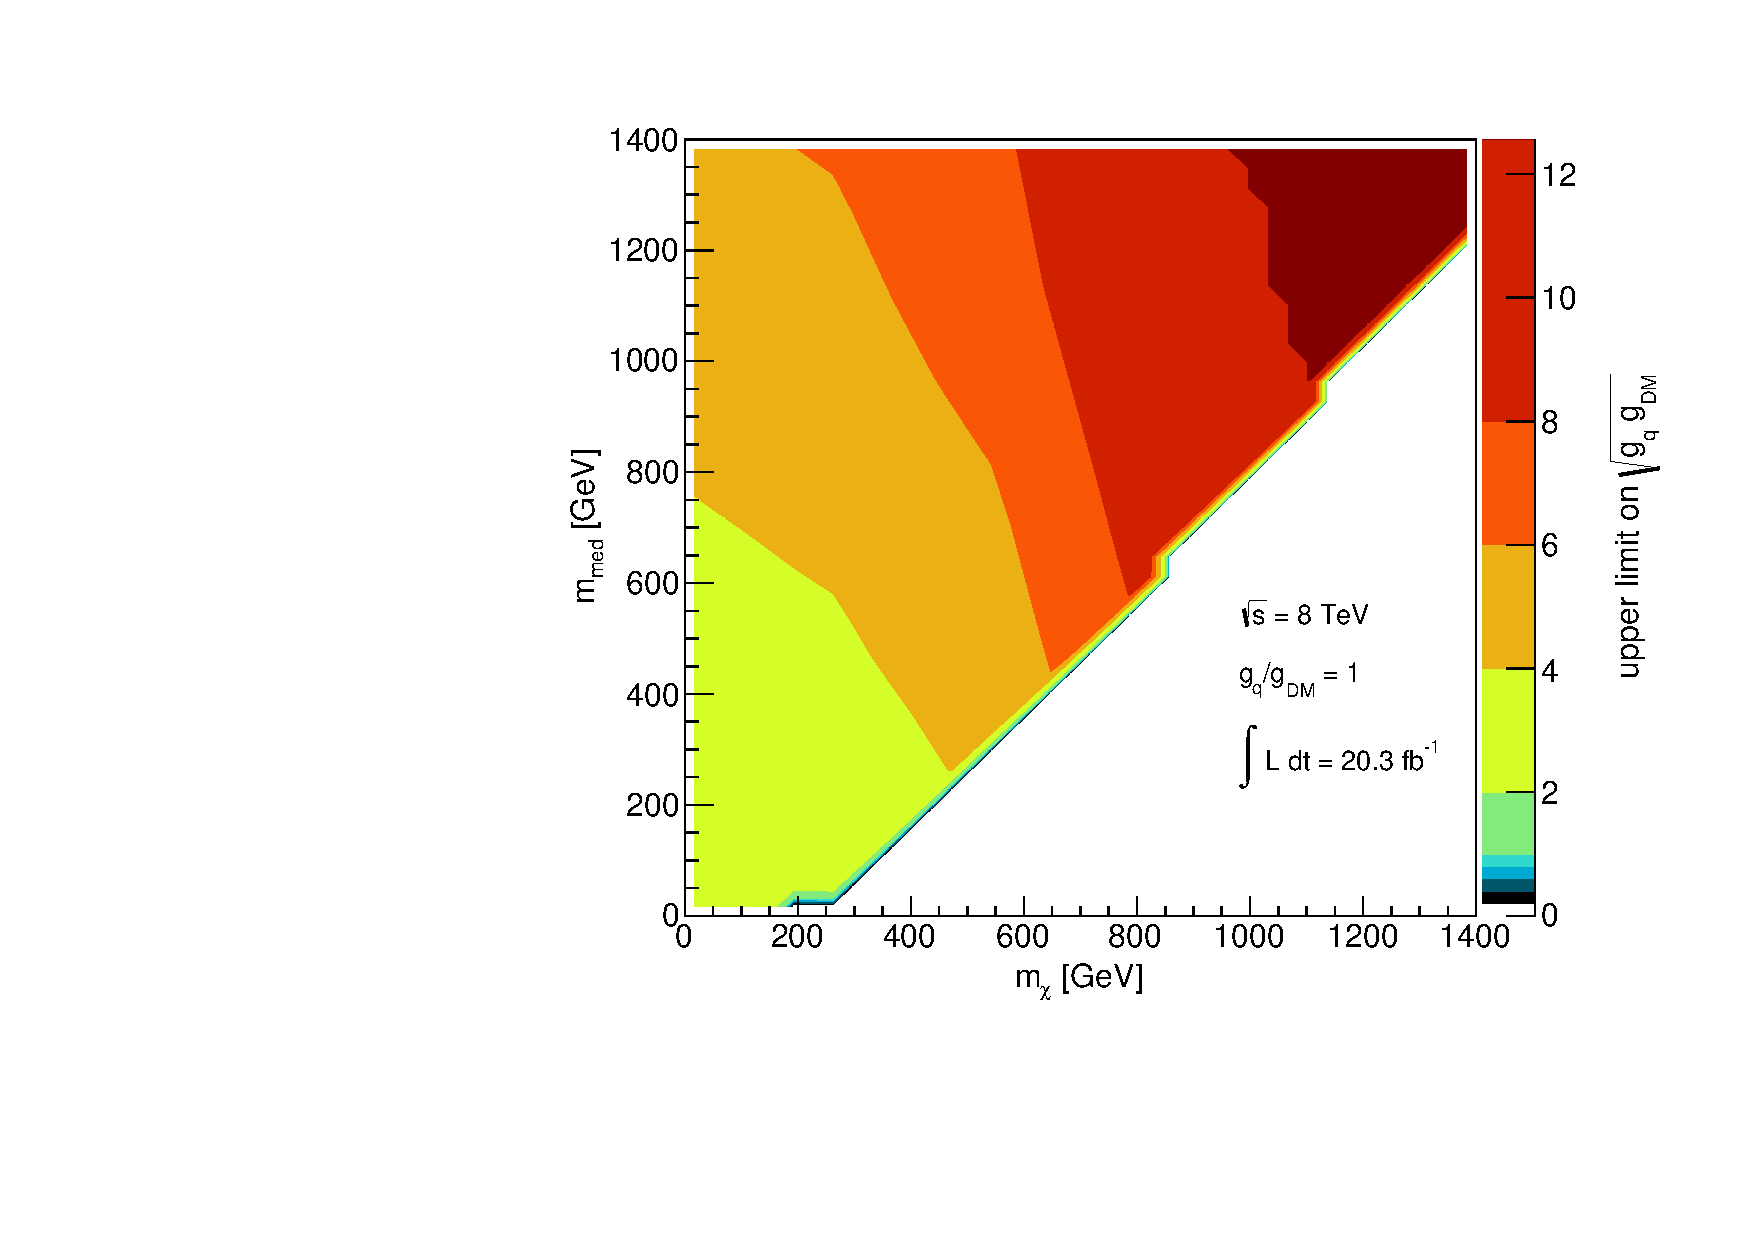
\includegraphics[width=0.45\textwidth]{figures/coupling_limits_TSD_1.pdf}
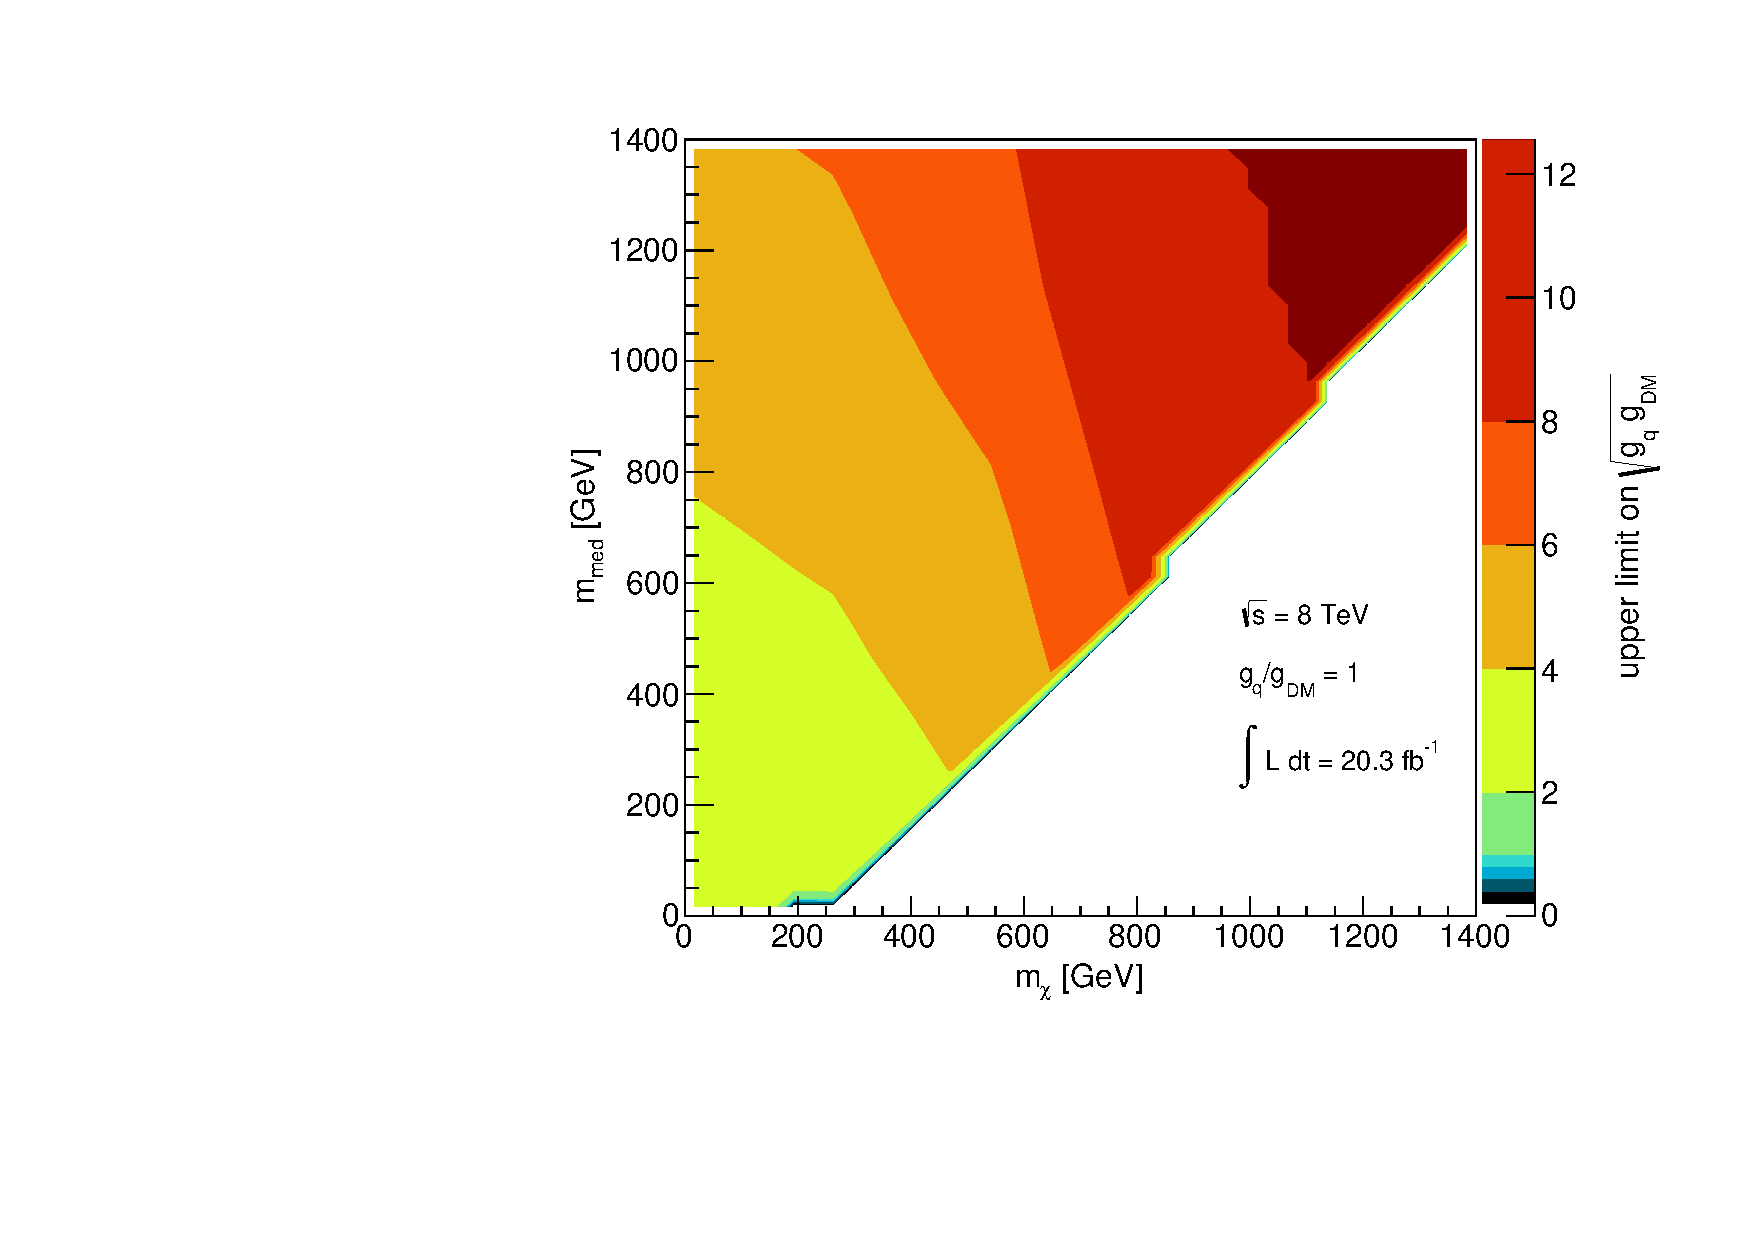
\includegraphics[width=0.45\textwidth]{figures/coupling_limits_TSD_1.pdf}
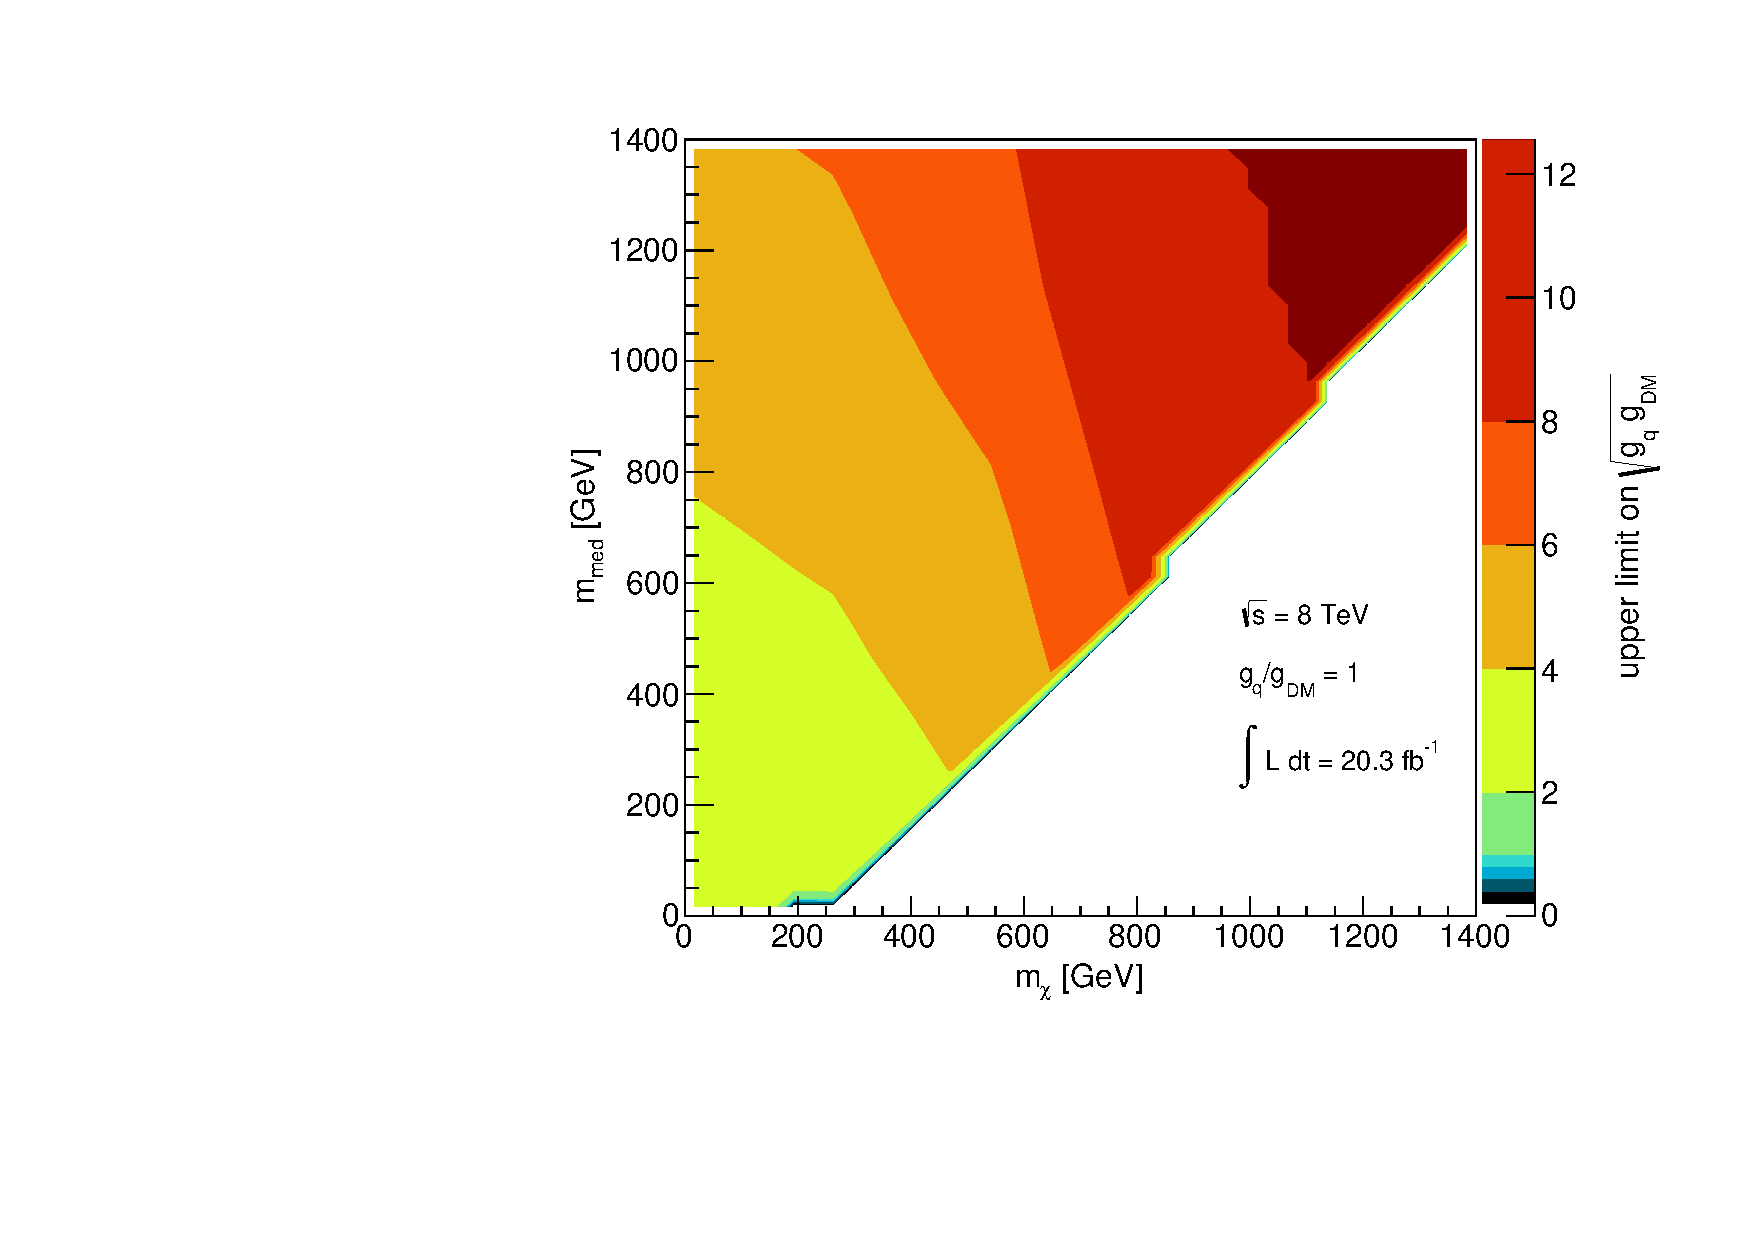
\includegraphics[width=0.45\textwidth]{figures/coupling_limits_TSD_1.pdf}
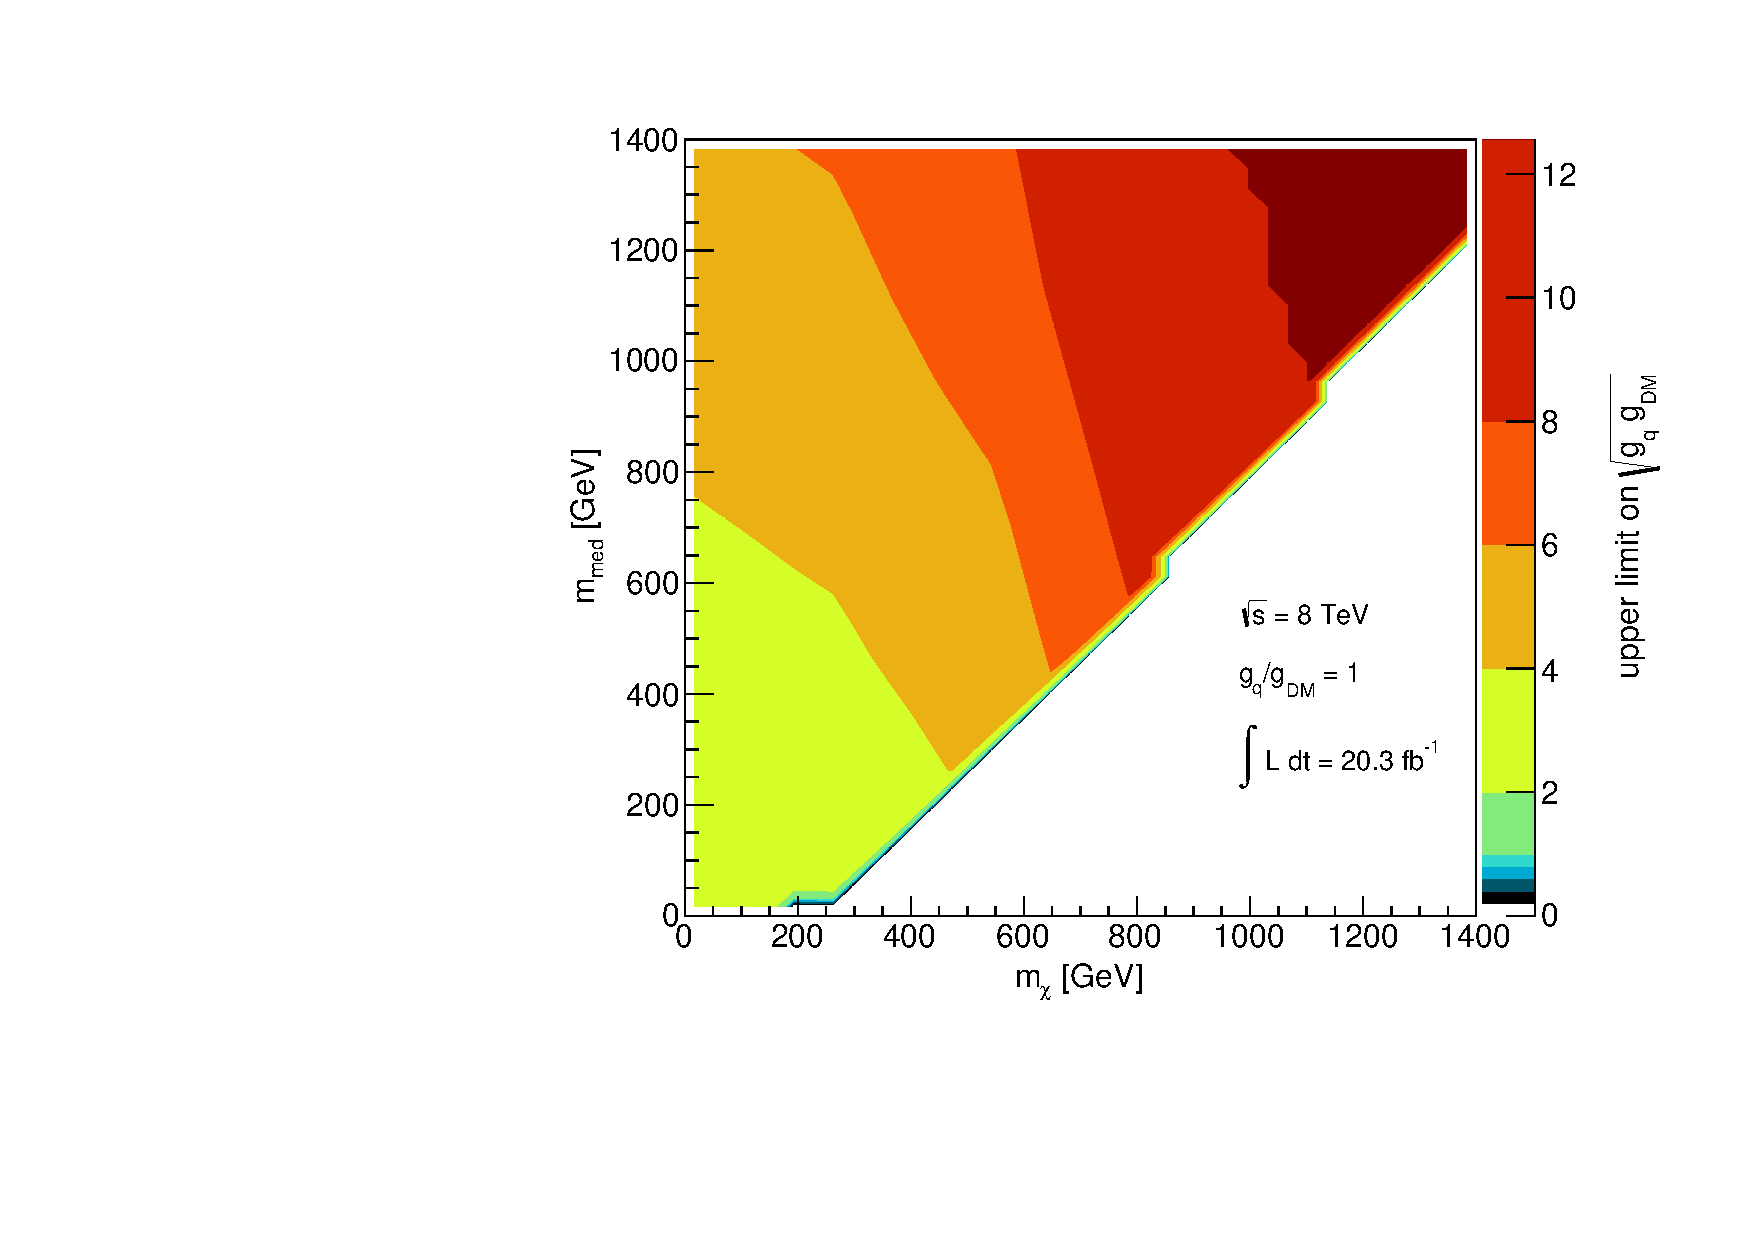
\includegraphics[width=0.45\textwidth]{figures/coupling_limits_TSD_1.pdf}
\caption{sS model coupling limit. REPLACE WITH SS MODEL PLOTS.}
\label{fig:Monojet_SSD_couplinglimit}
\end{center}
\end{figure}

\begin{figure}[!h]
\begin{center}
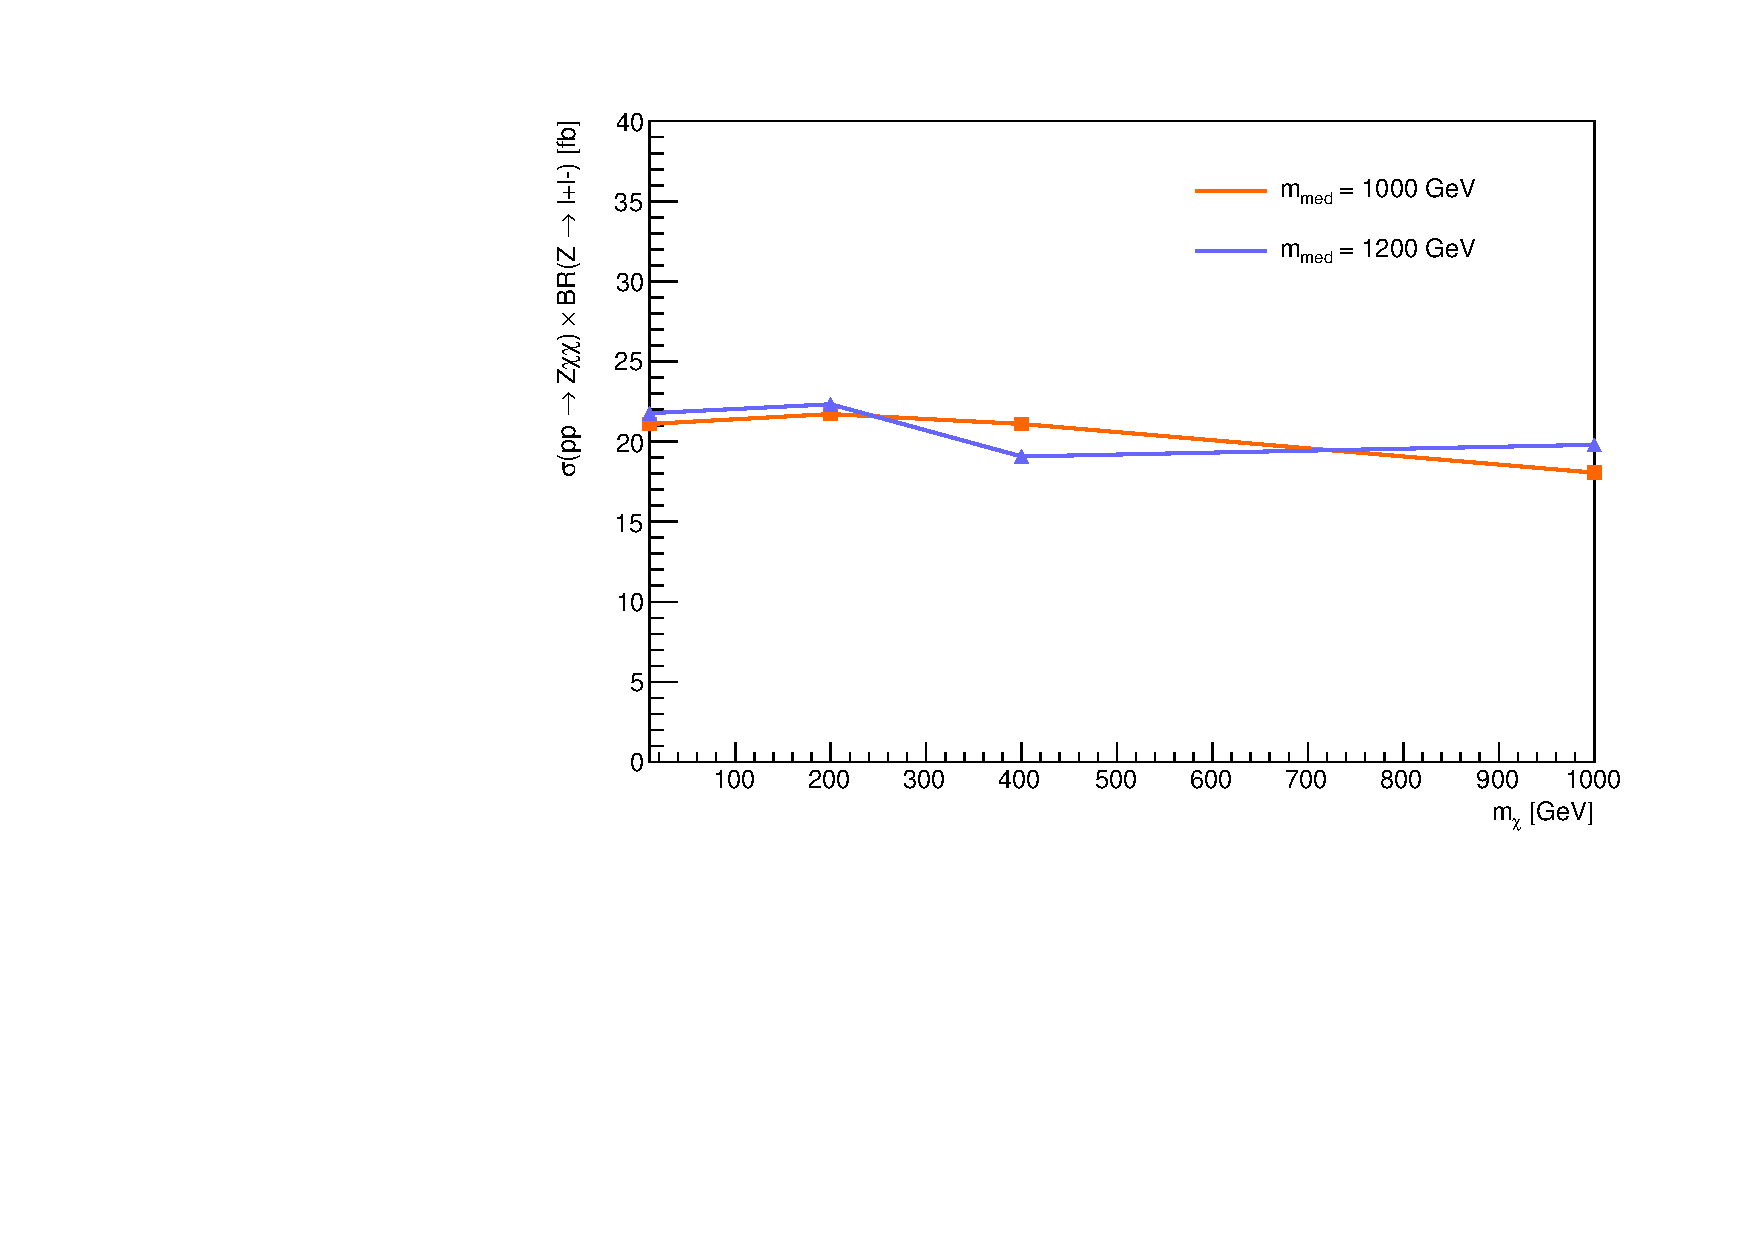
\includegraphics[width=0.45\textwidth]{figures/monoZ_sigma_limits_variedDMmass.pdf}
\caption{Mono-Z channel, tS model. REPLACE WITH TS MODEL PLOTS.}
\label{fig:MonoZ_TSD_limit}
\end{center} 
\end{figure}

\begin{figure}[!h]
\begin{center}
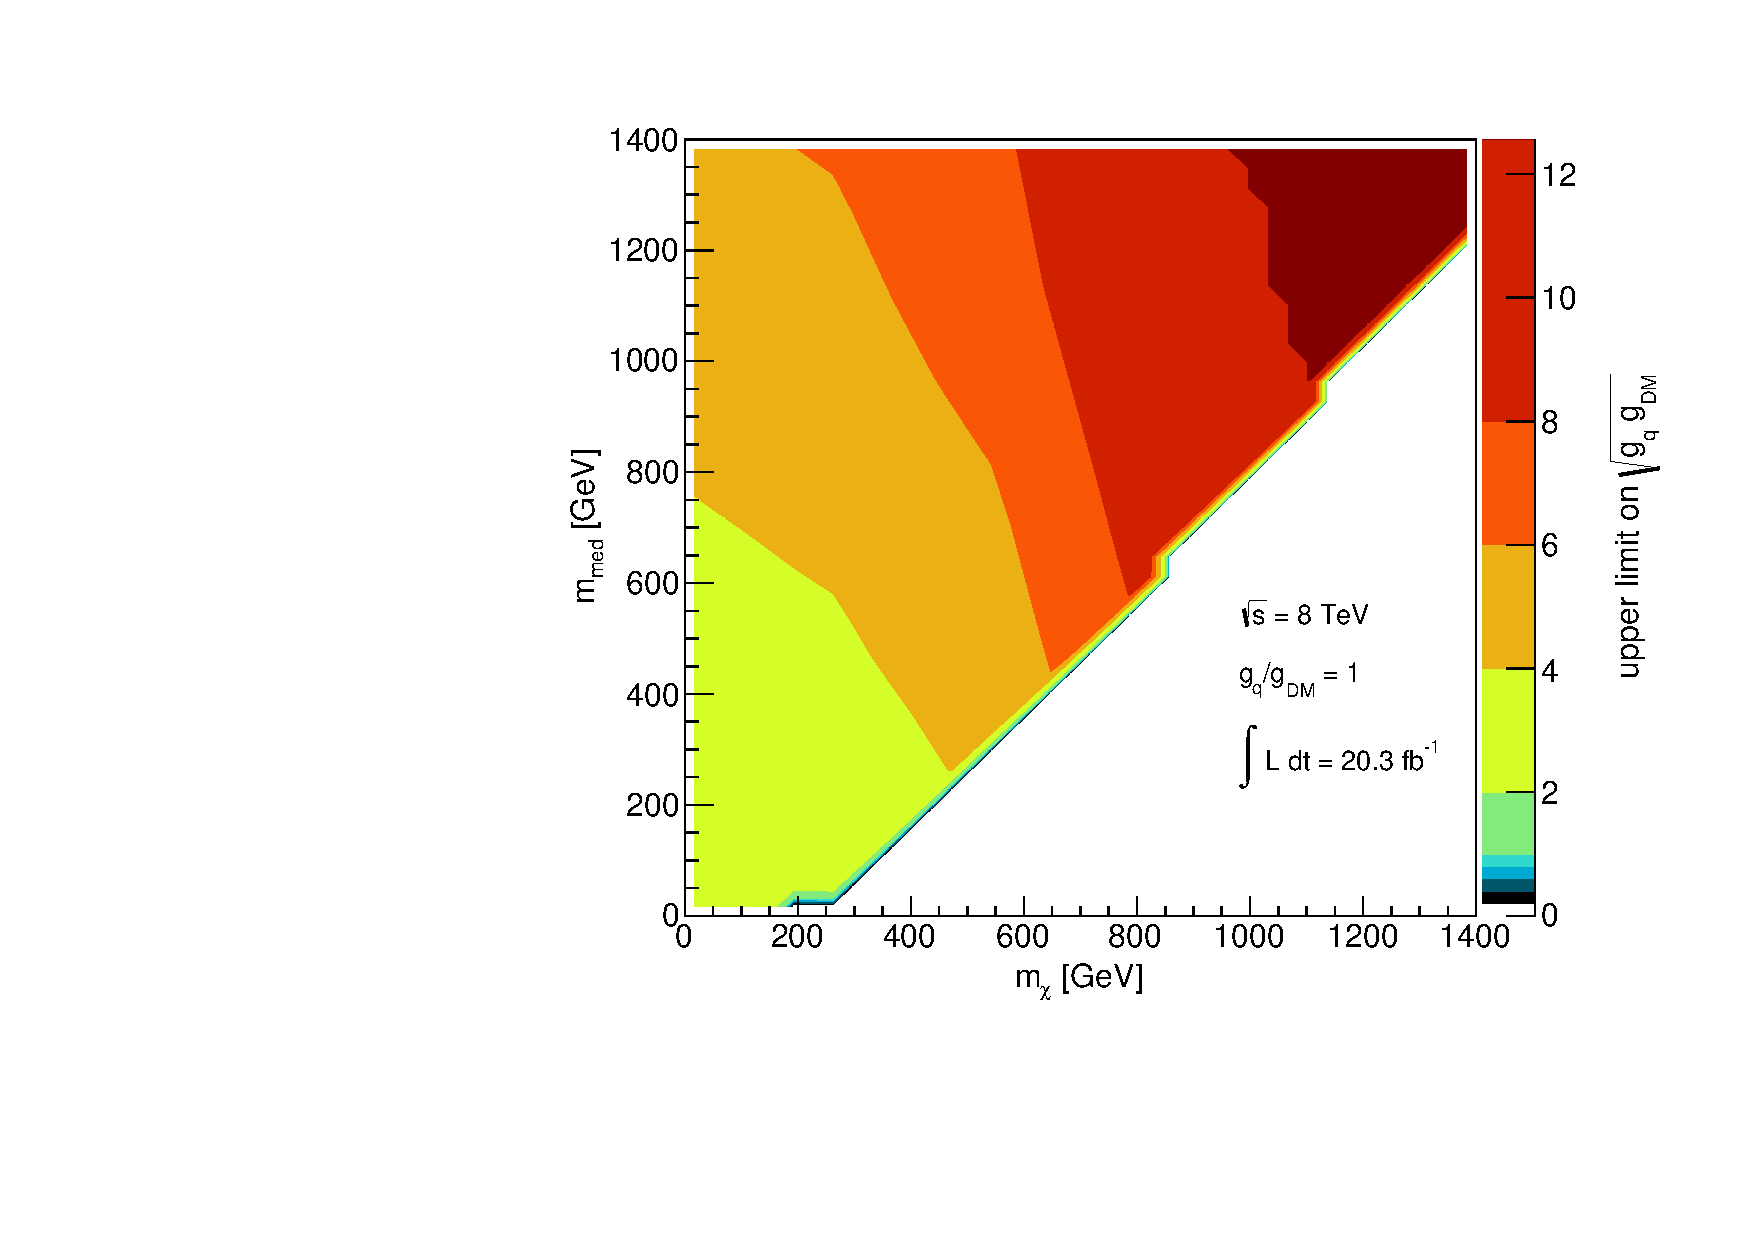
\includegraphics[width=0.45\textwidth]{figures/coupling_limits_TSD_1.pdf}
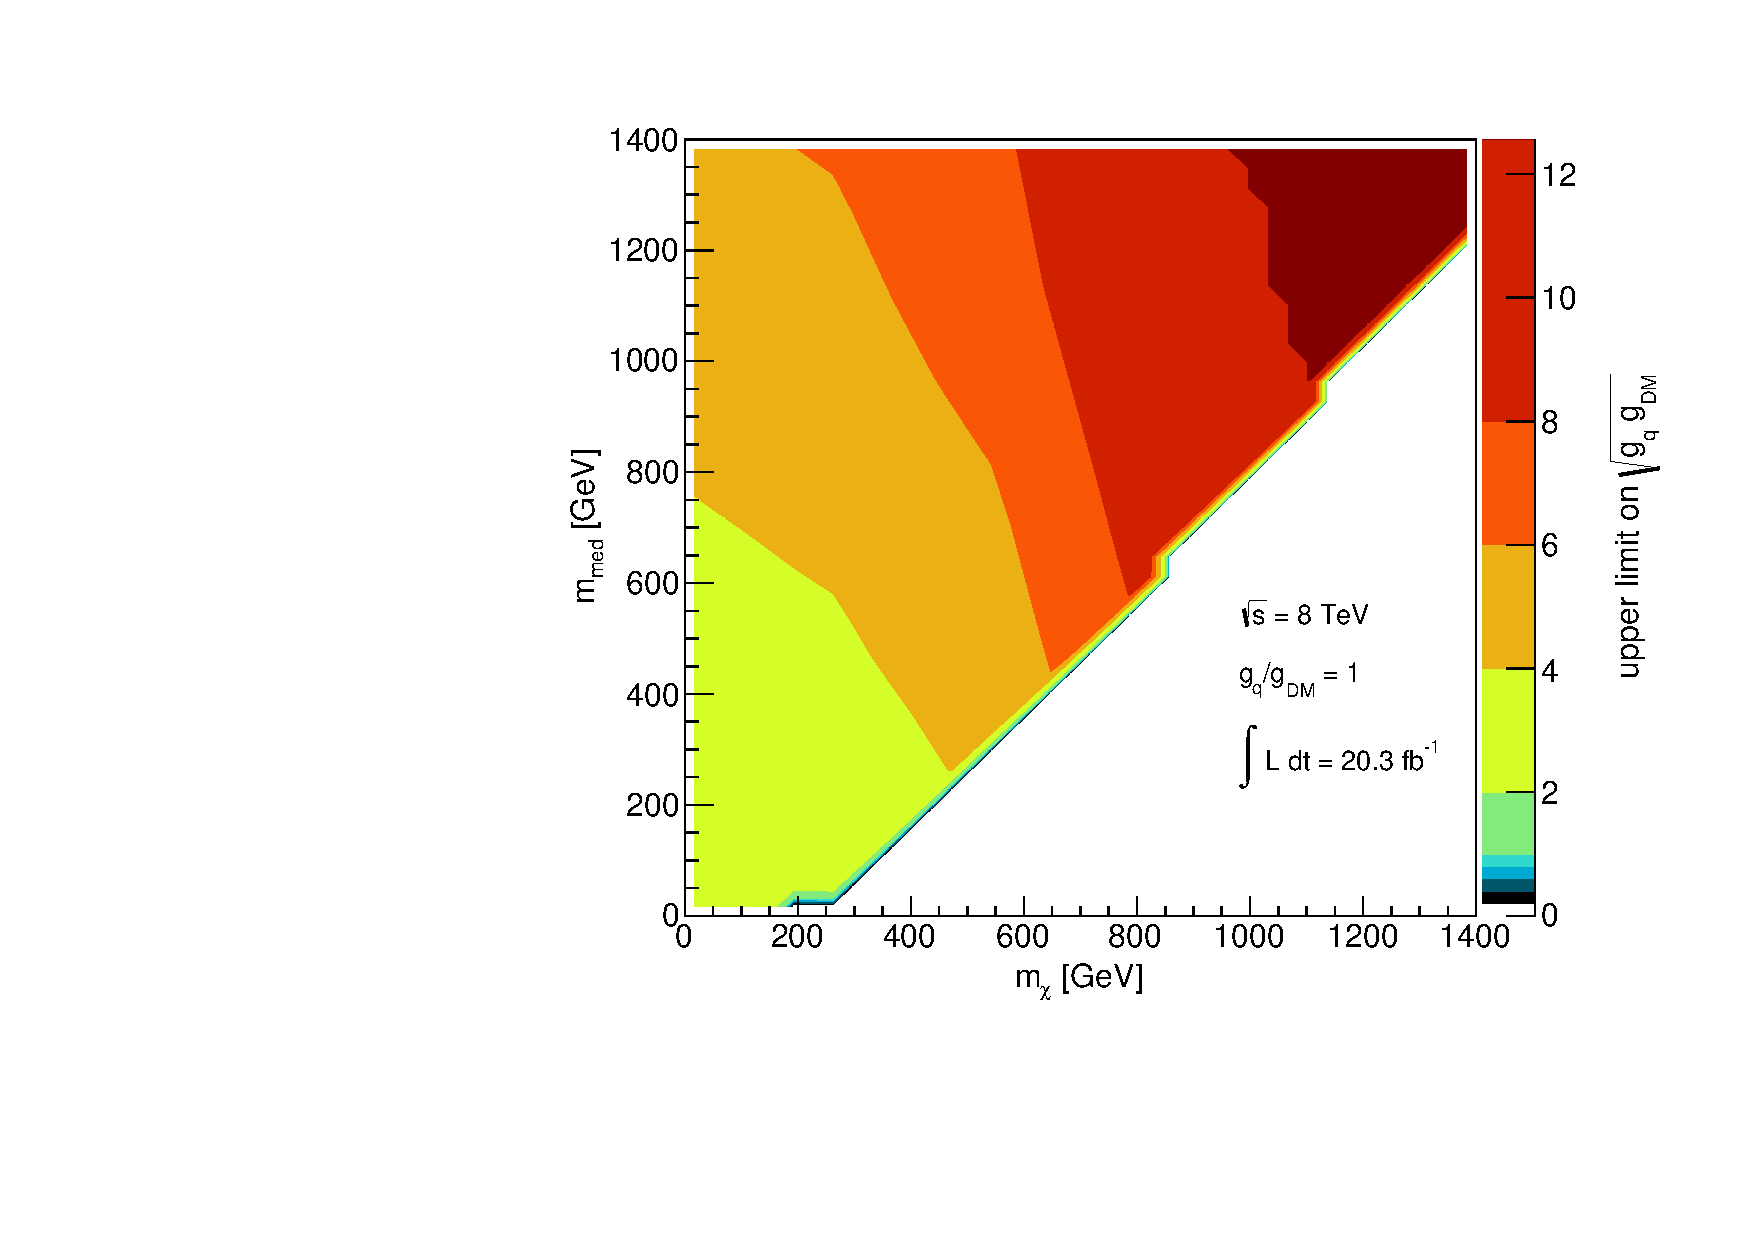
\includegraphics[width=0.45\textwidth]{figures/coupling_limits_TSD_1.pdf}
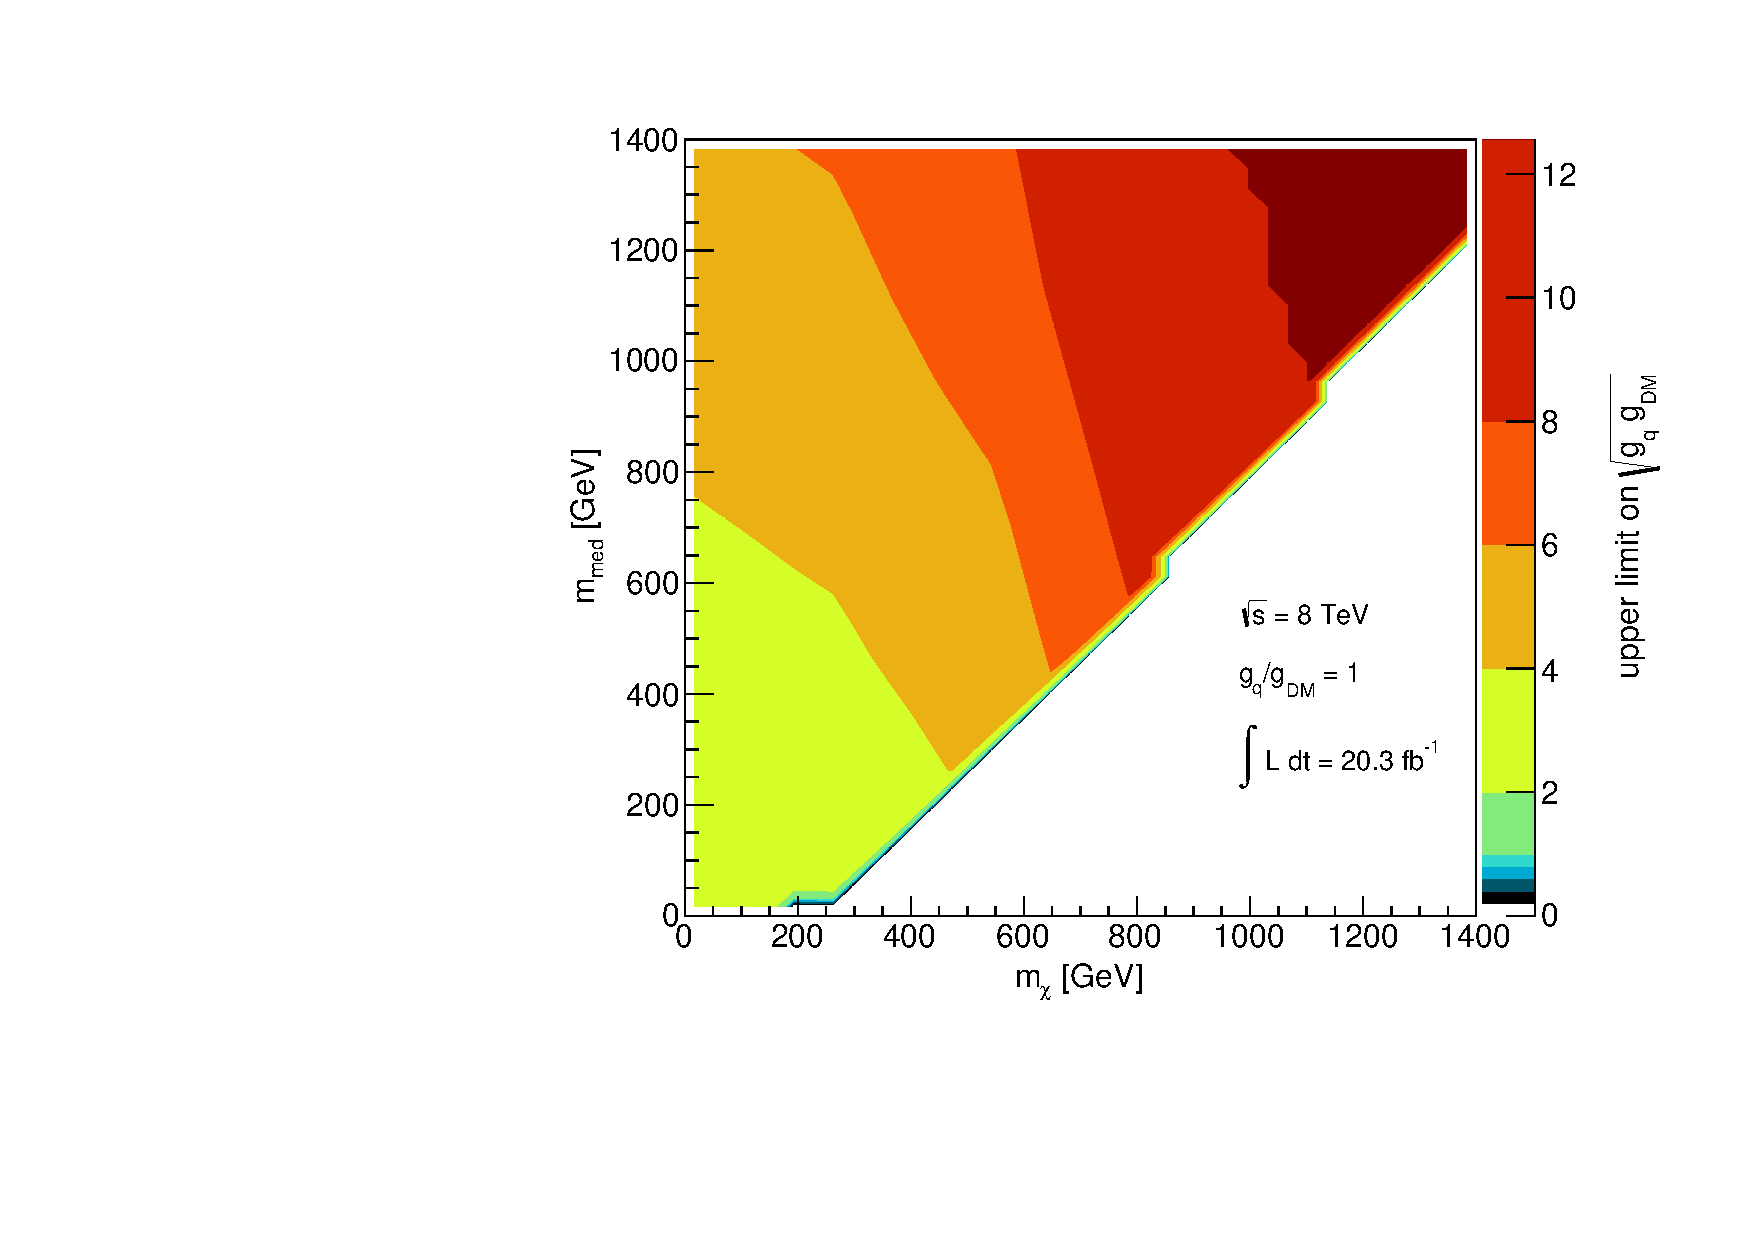
\includegraphics[width=0.45\textwidth]{figures/coupling_limits_TSD_1.pdf}
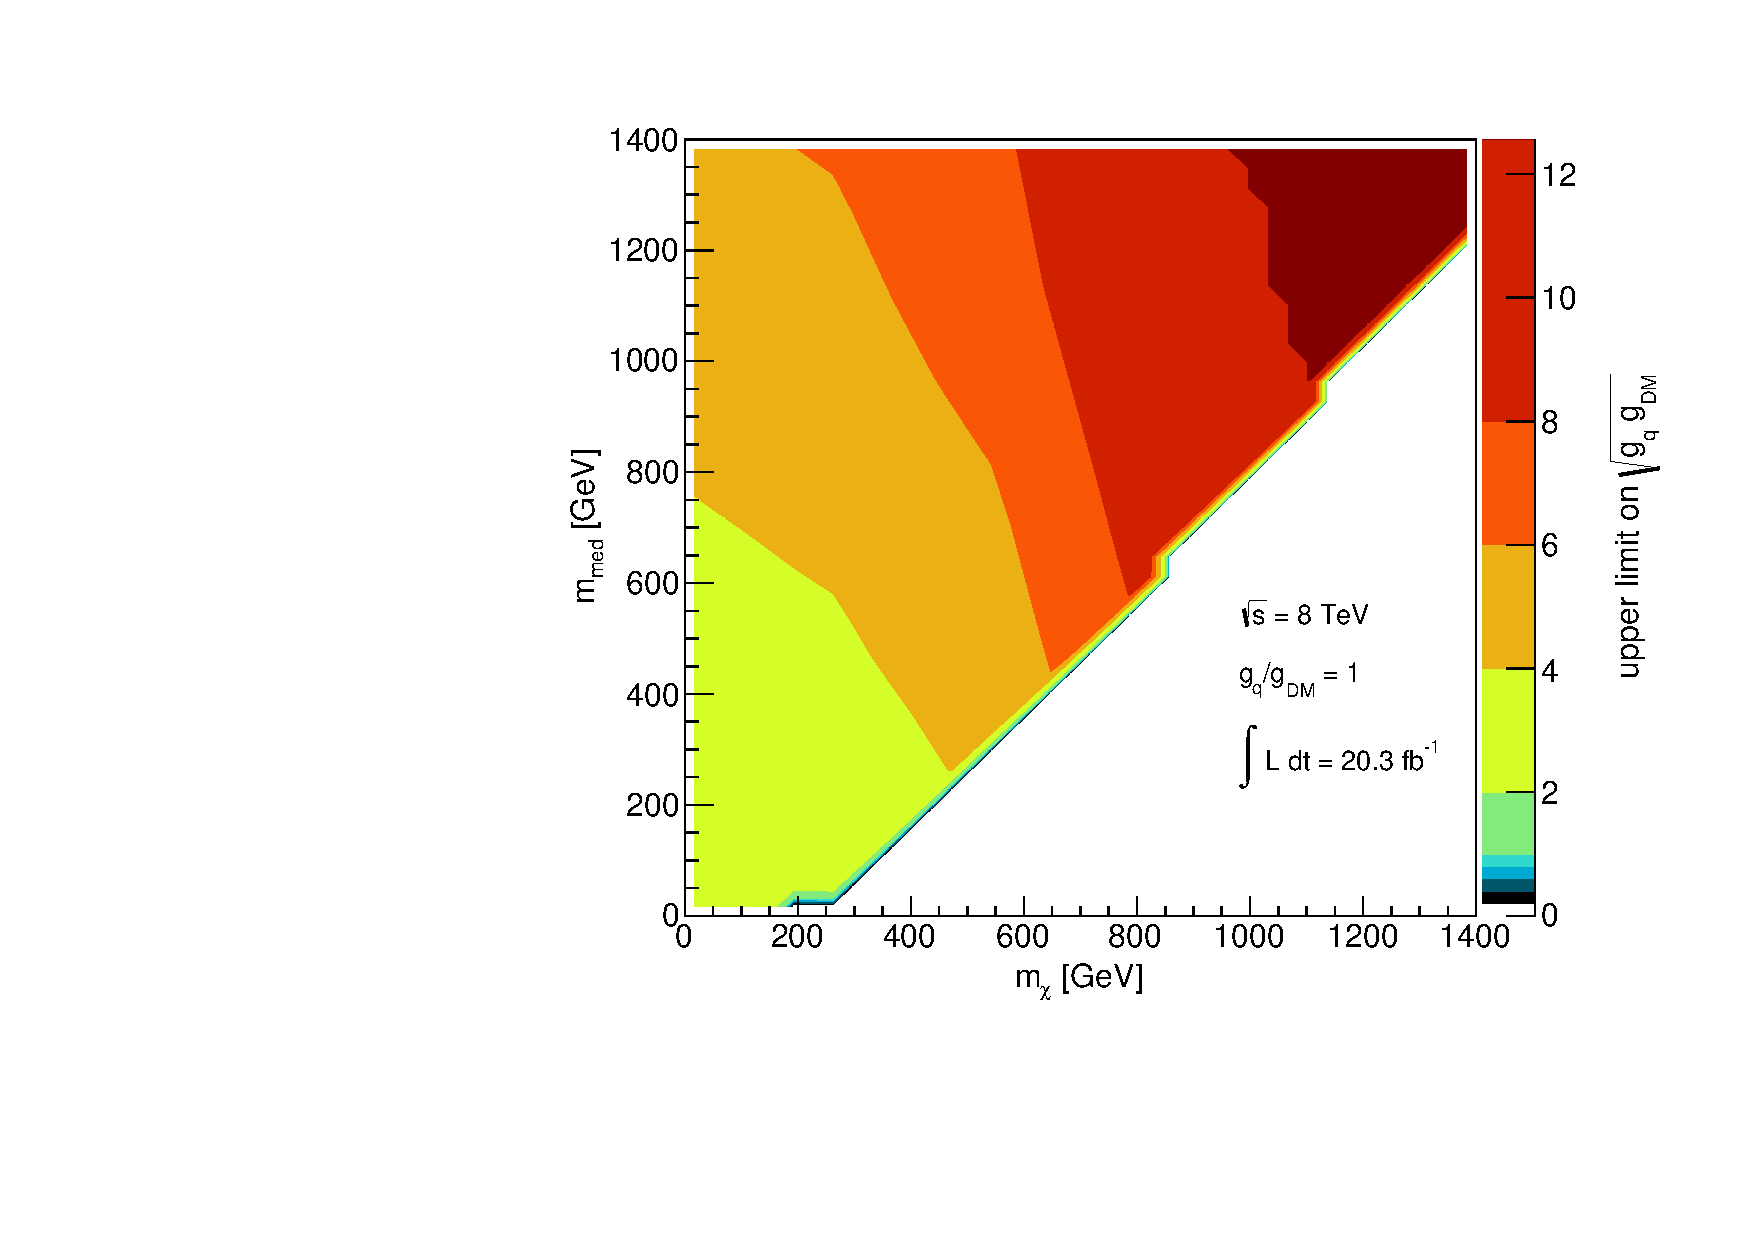
\includegraphics[width=0.45\textwidth]{figures/coupling_limits_TSD_1.pdf}
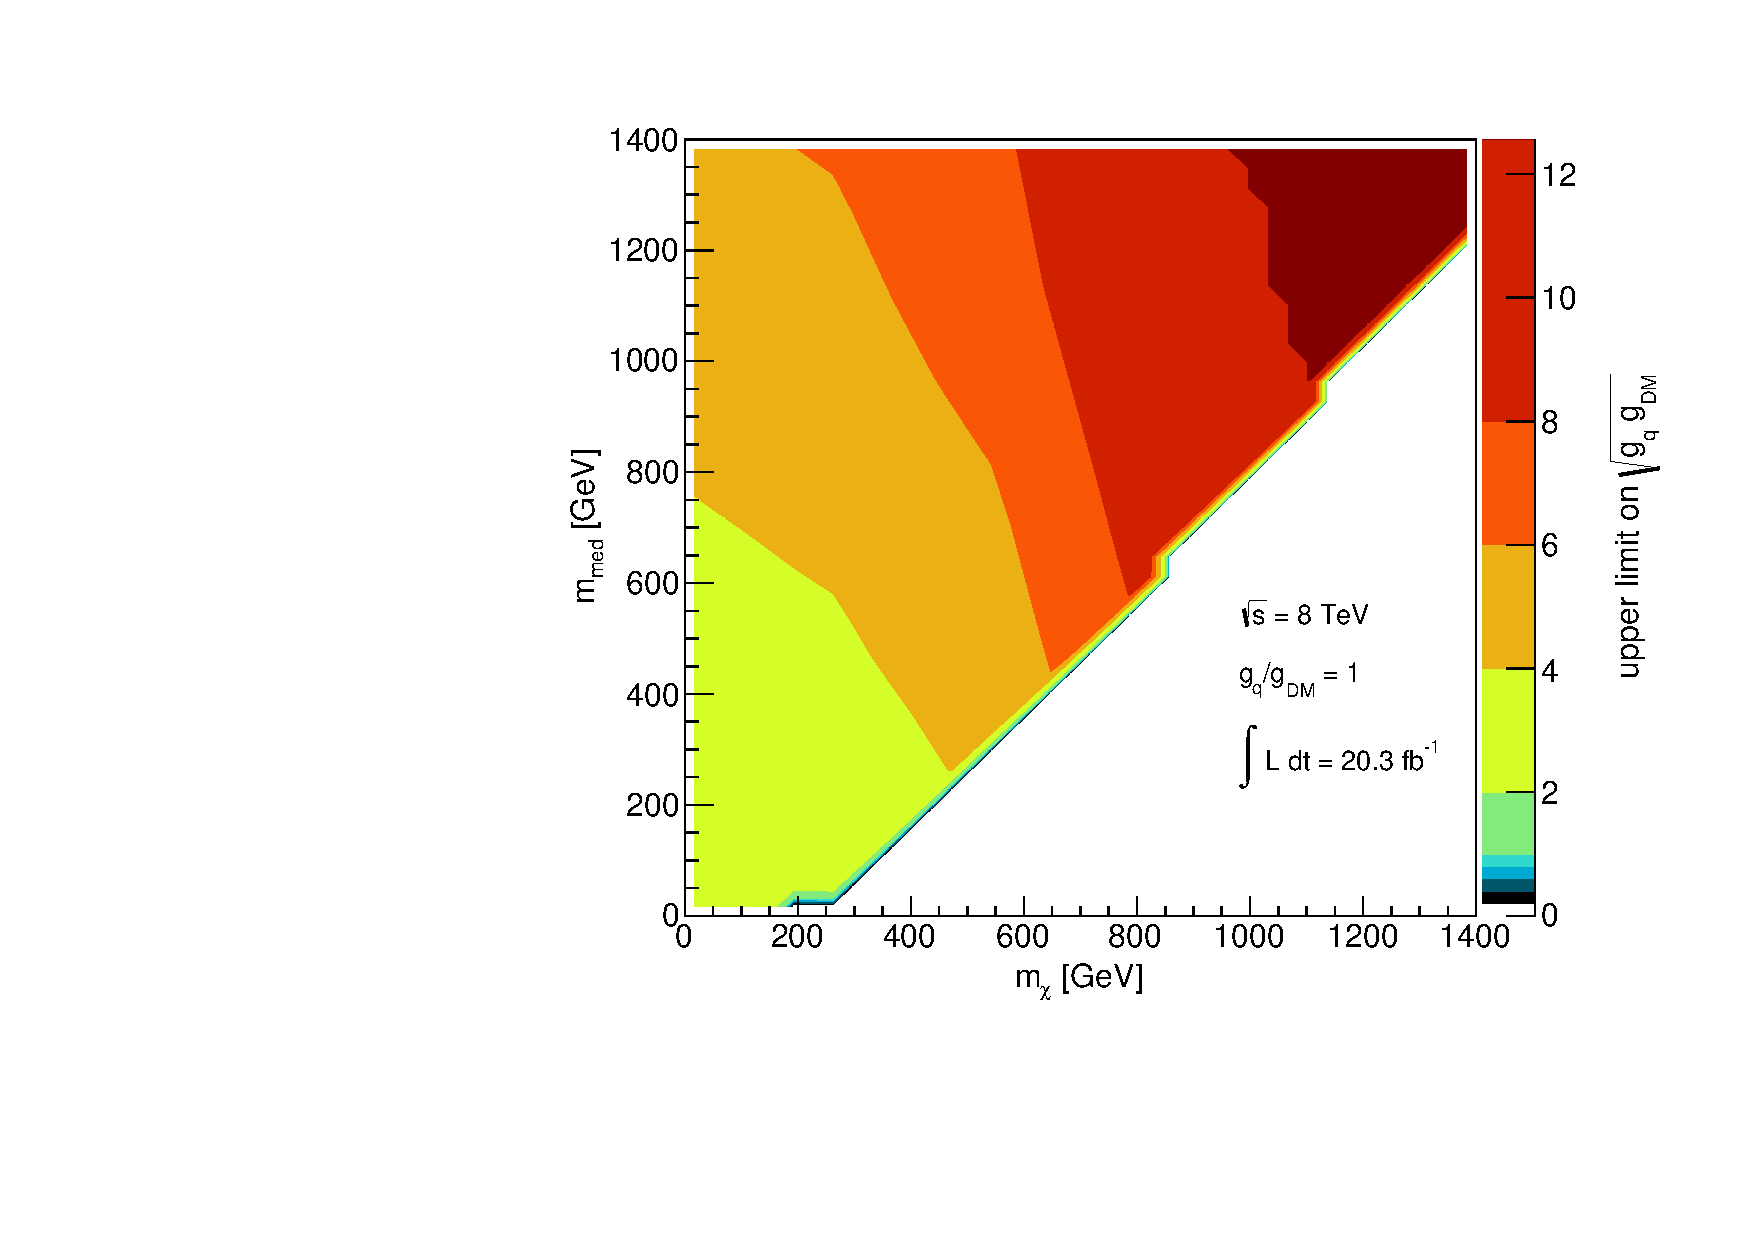
\includegraphics[width=0.45\textwidth]{figures/coupling_limits_TSD_1.pdf}
\caption{tS model coupling limit. REPLACE WITH TS MODEL PLOTS.}
\label{fig:MonoZ_TSD_couplinglimit}
\end{center}
\end{figure}

\subsection{Mono-$Z$ channel}

\begin{figure}[!h]
\begin{center}
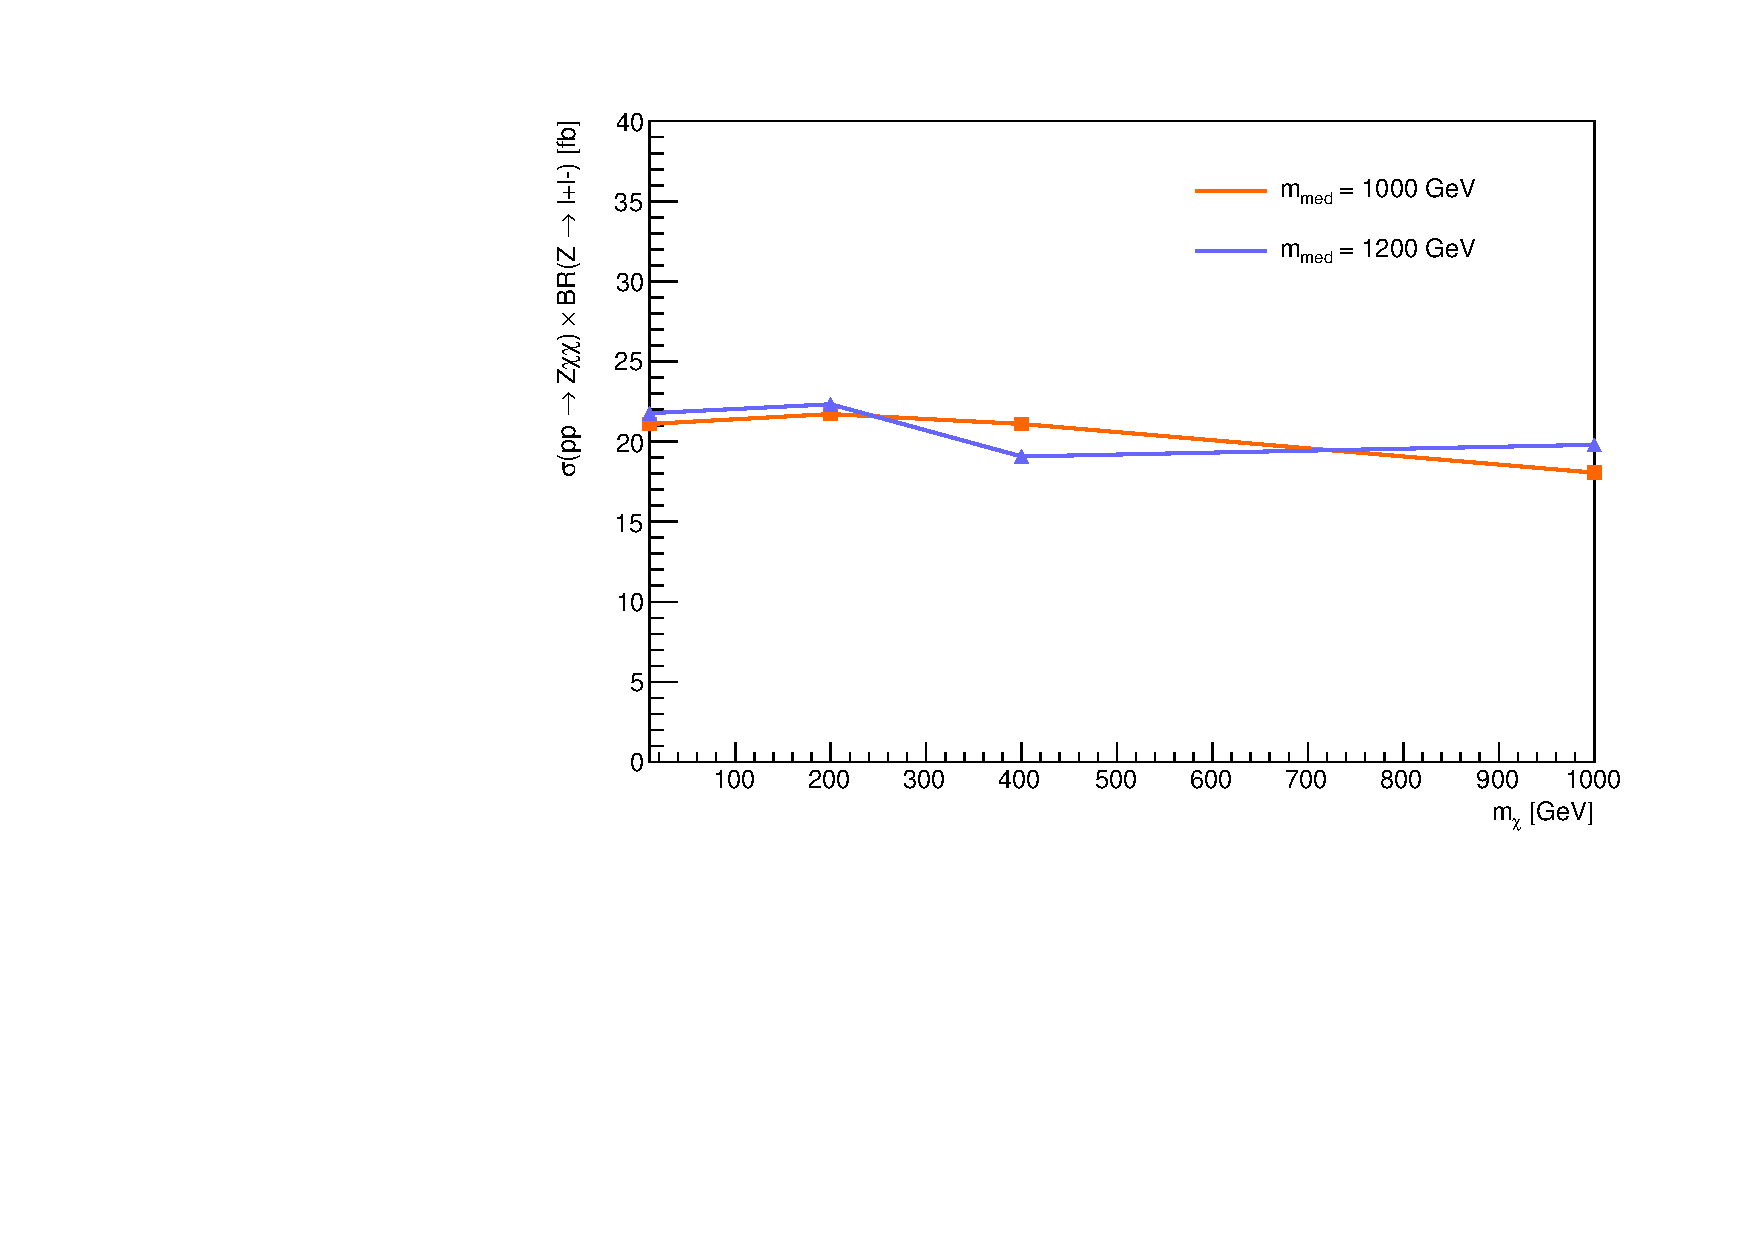
\includegraphics[width=0.45\textwidth]{figures/monoZ_sigma_limits_variedDMmass.pdf}
\caption{A very rough first plot - to be prettified! Shows the limit on sigma x BR for the sV model in the mono-Z channel. Will change to have a band for the expected limit, and a line for the observed limit. Show 5 different coupling scenarios on one plot. Mono-Z channel, sV model.}
\label{fig:MonoZ_SVD_limit}
\end{center}
\end{figure}

\begin{figure}[!h]
\begin{center}
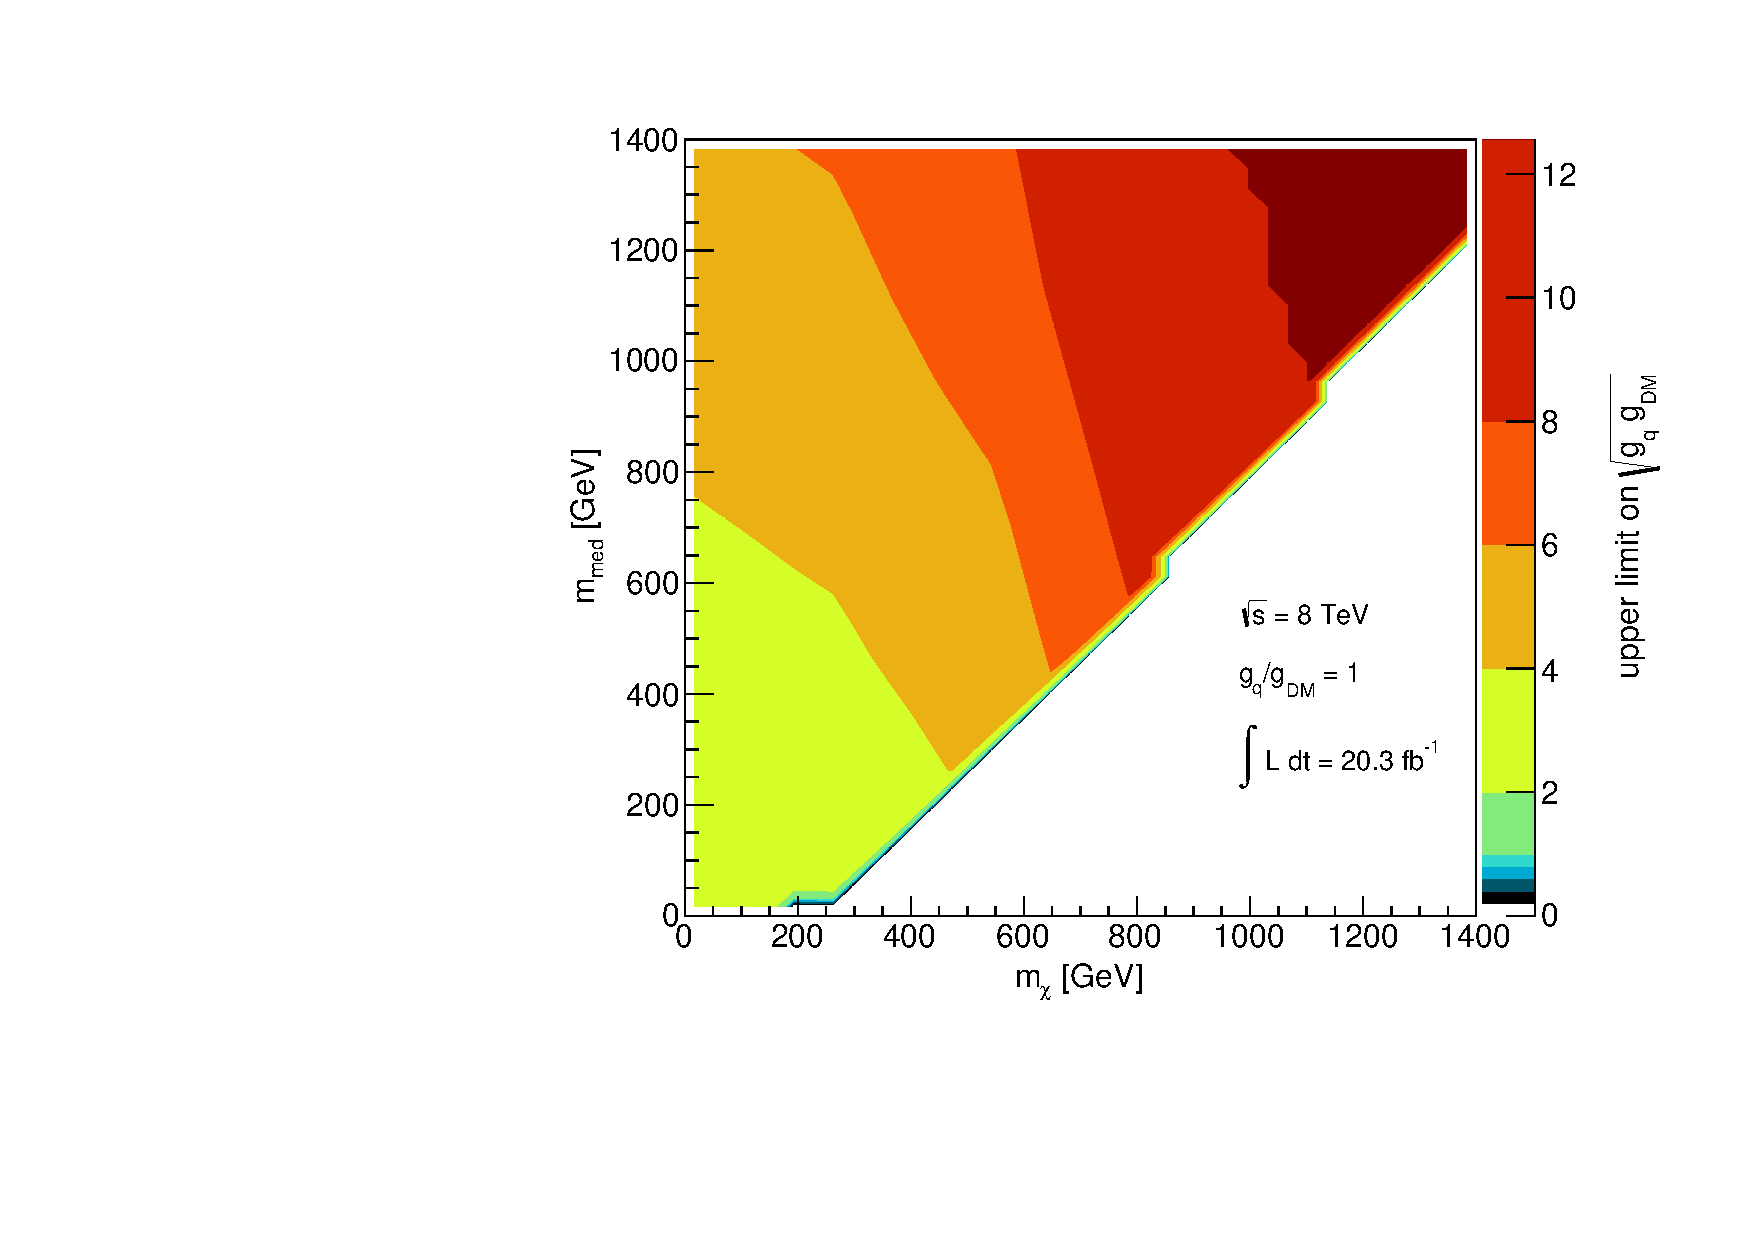
\includegraphics[width=0.45\textwidth]{figures/coupling_limits_TSD_1.pdf}
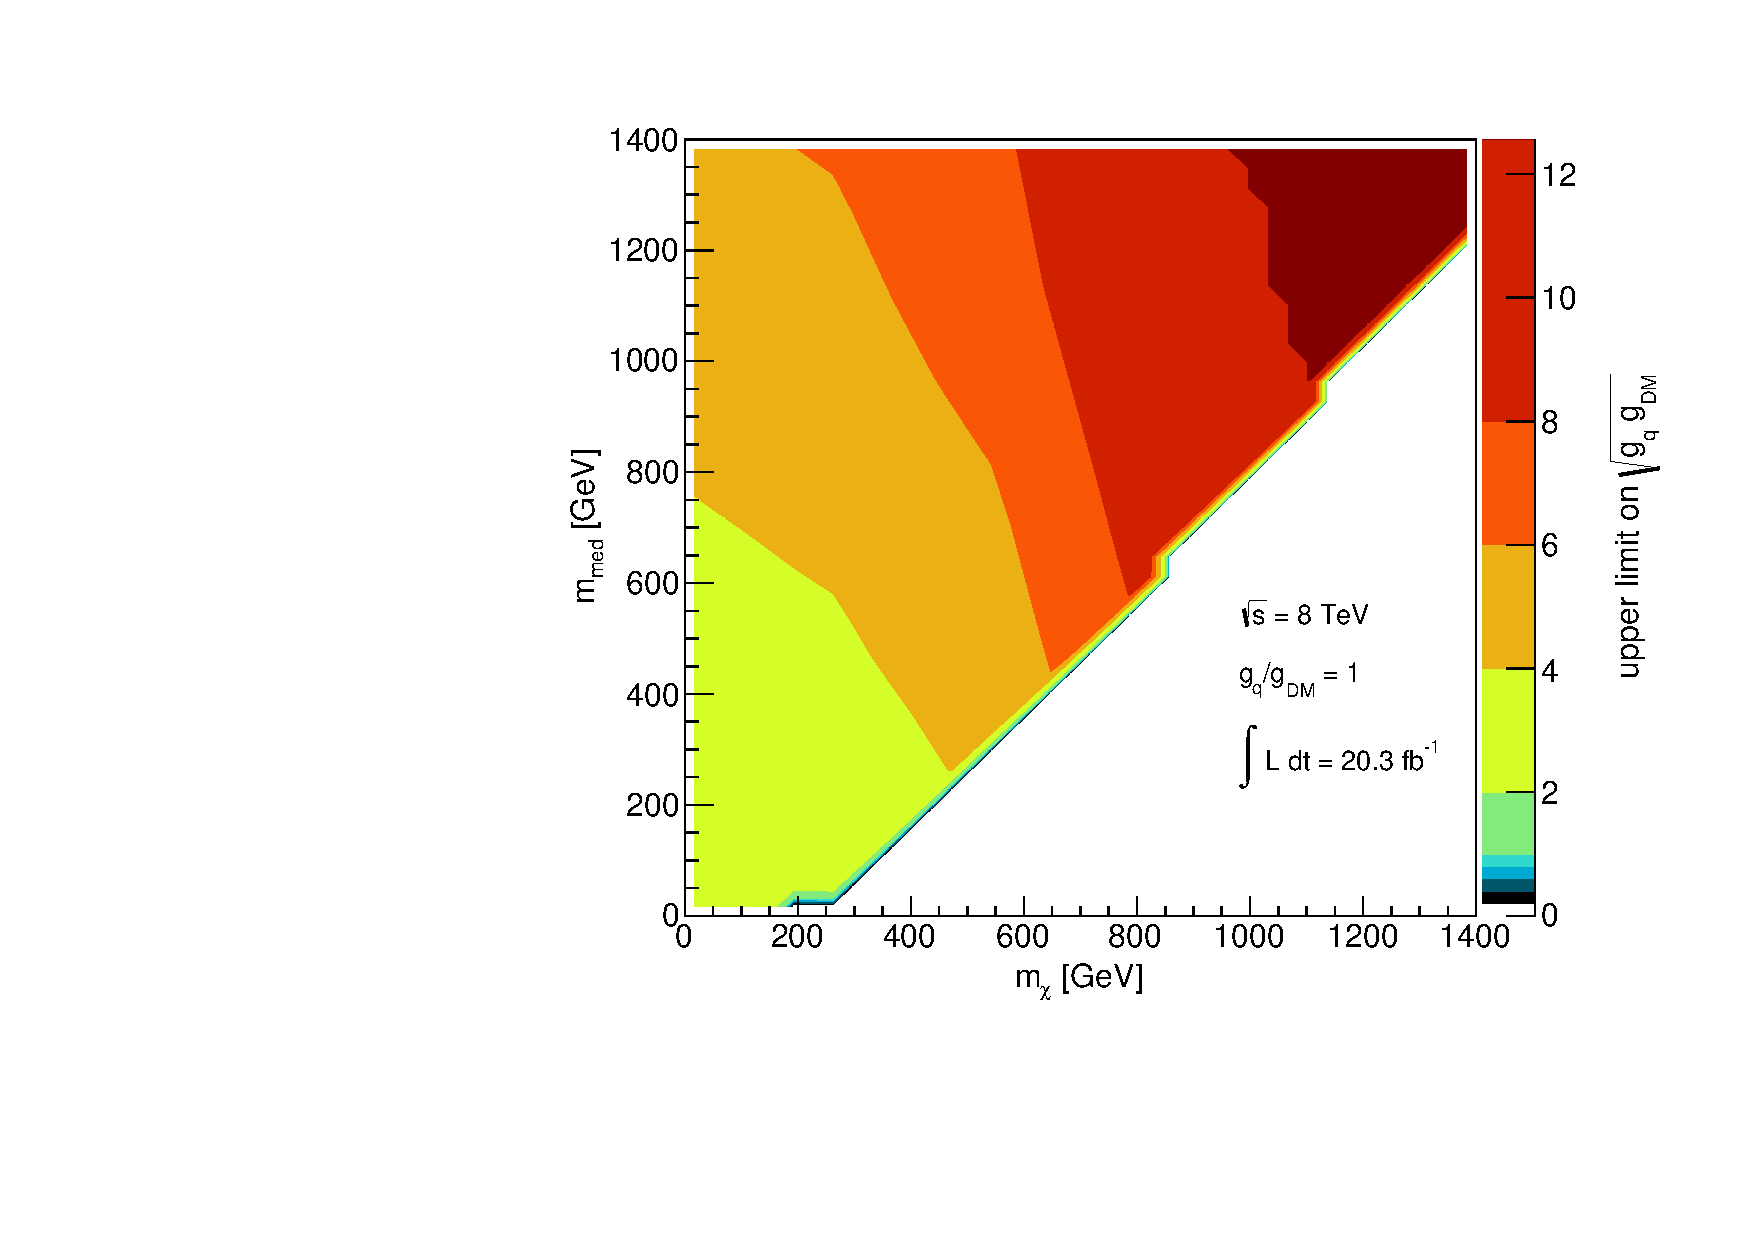
\includegraphics[width=0.45\textwidth]{figures/coupling_limits_TSD_1.pdf}
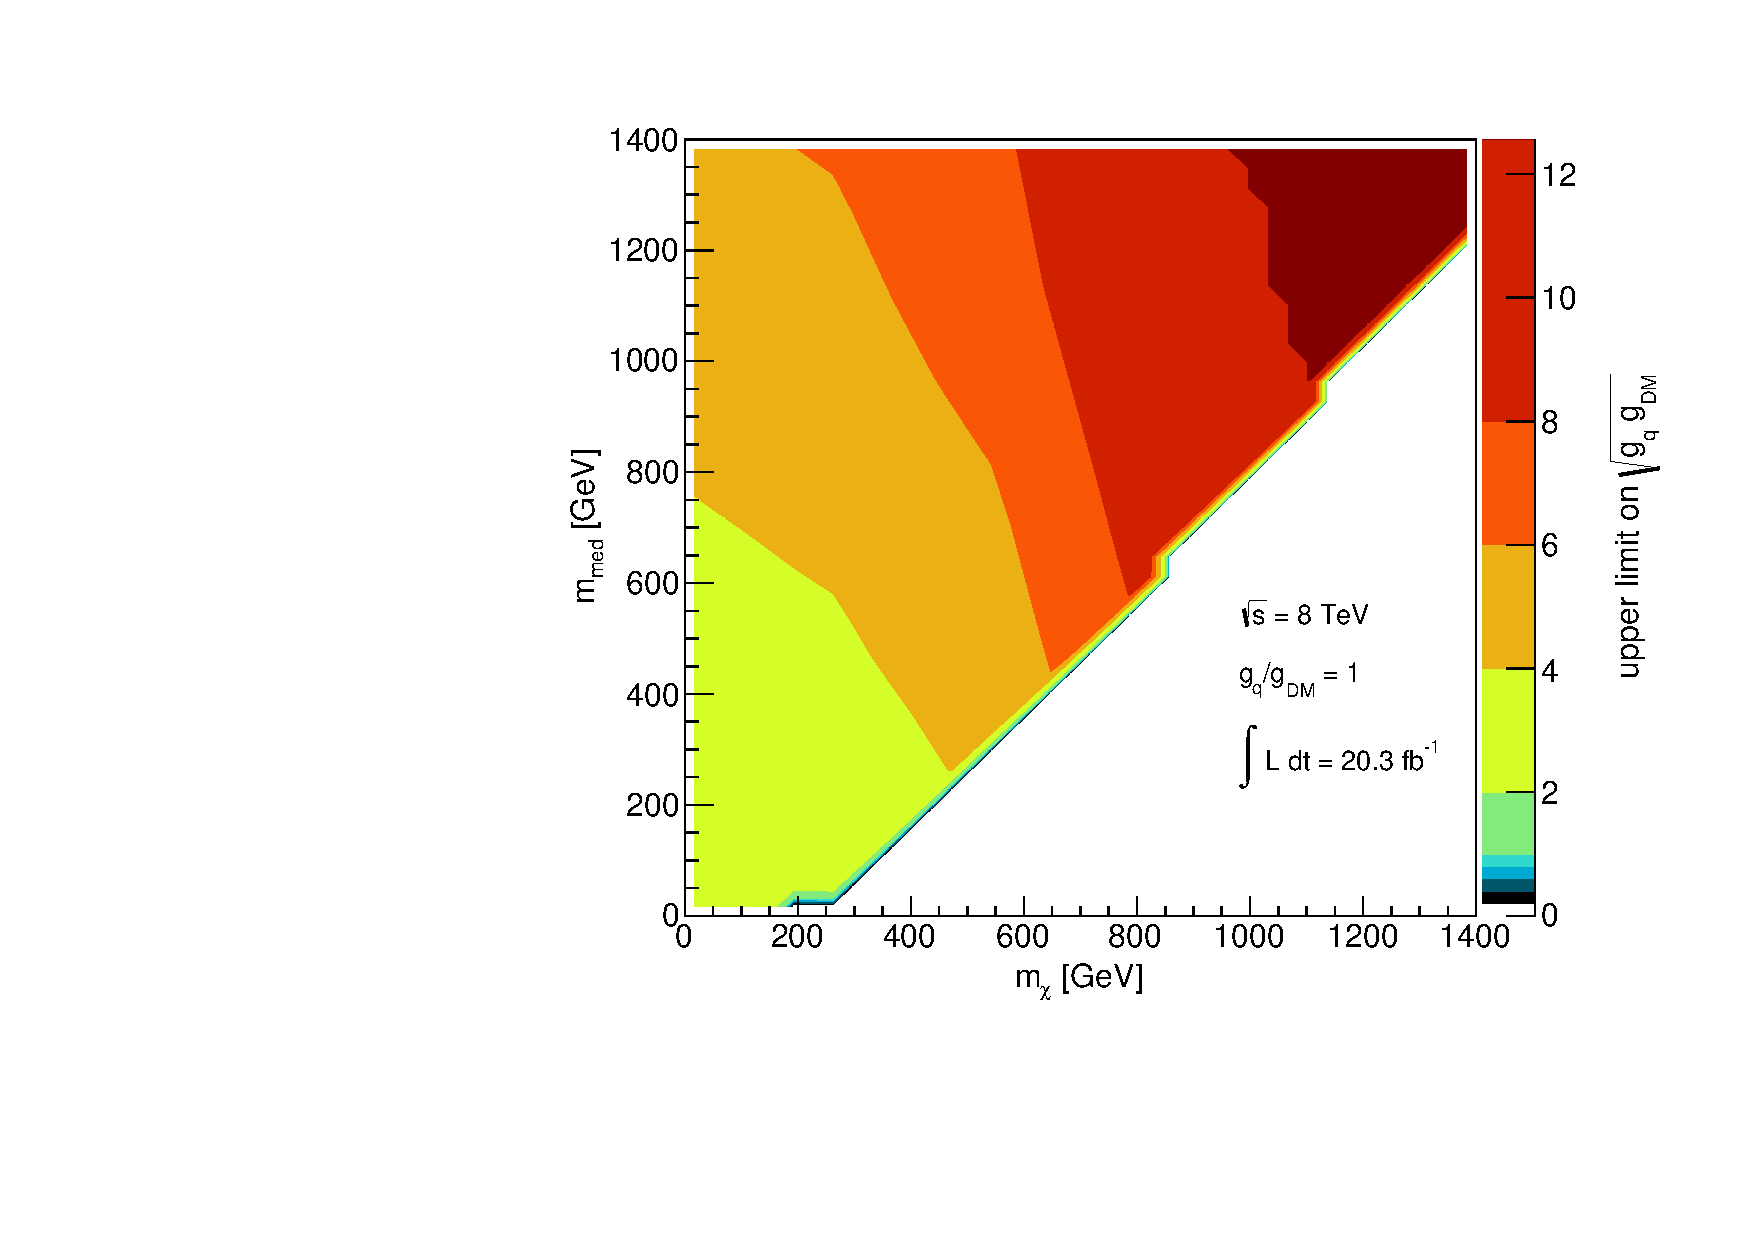
\includegraphics[width=0.45\textwidth]{figures/coupling_limits_TSD_1.pdf}
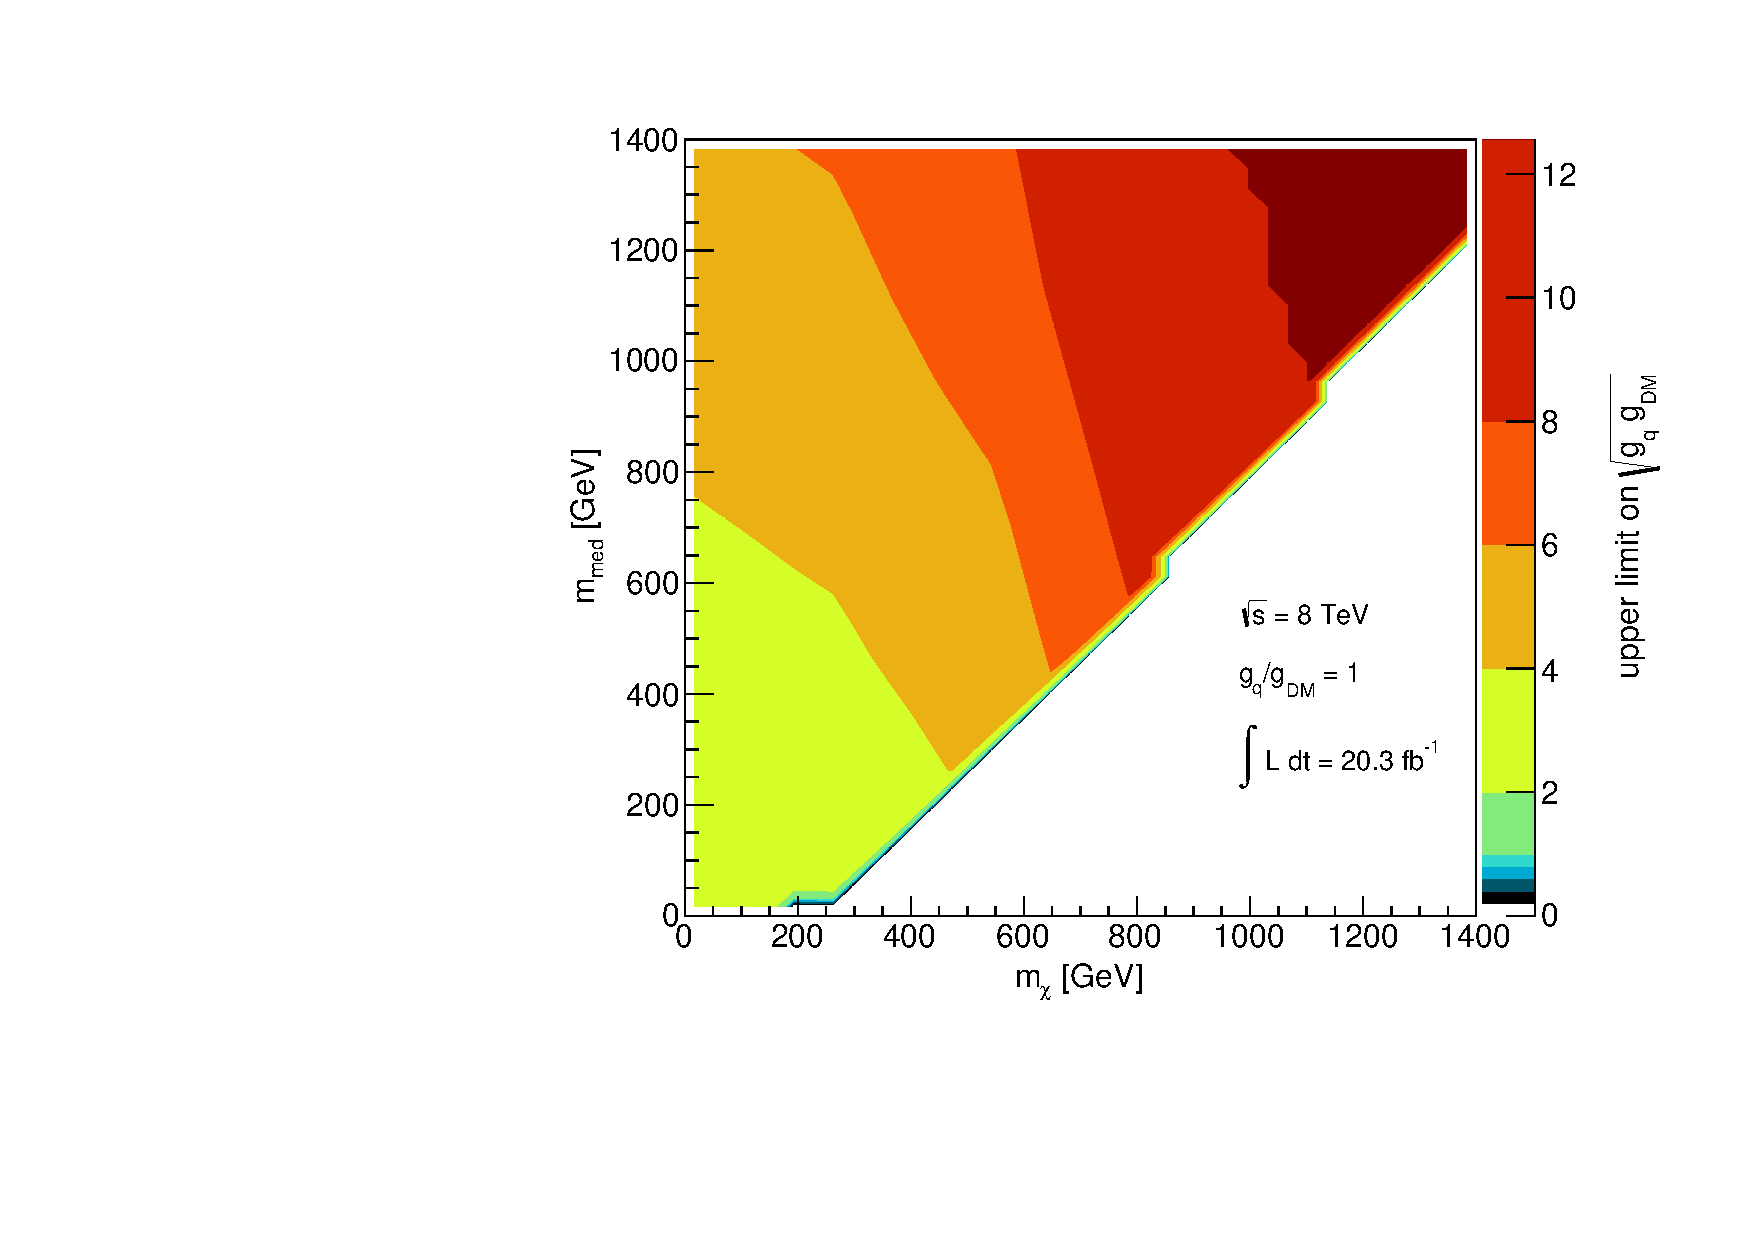
\includegraphics[width=0.45\textwidth]{figures/coupling_limits_TSD_1.pdf}
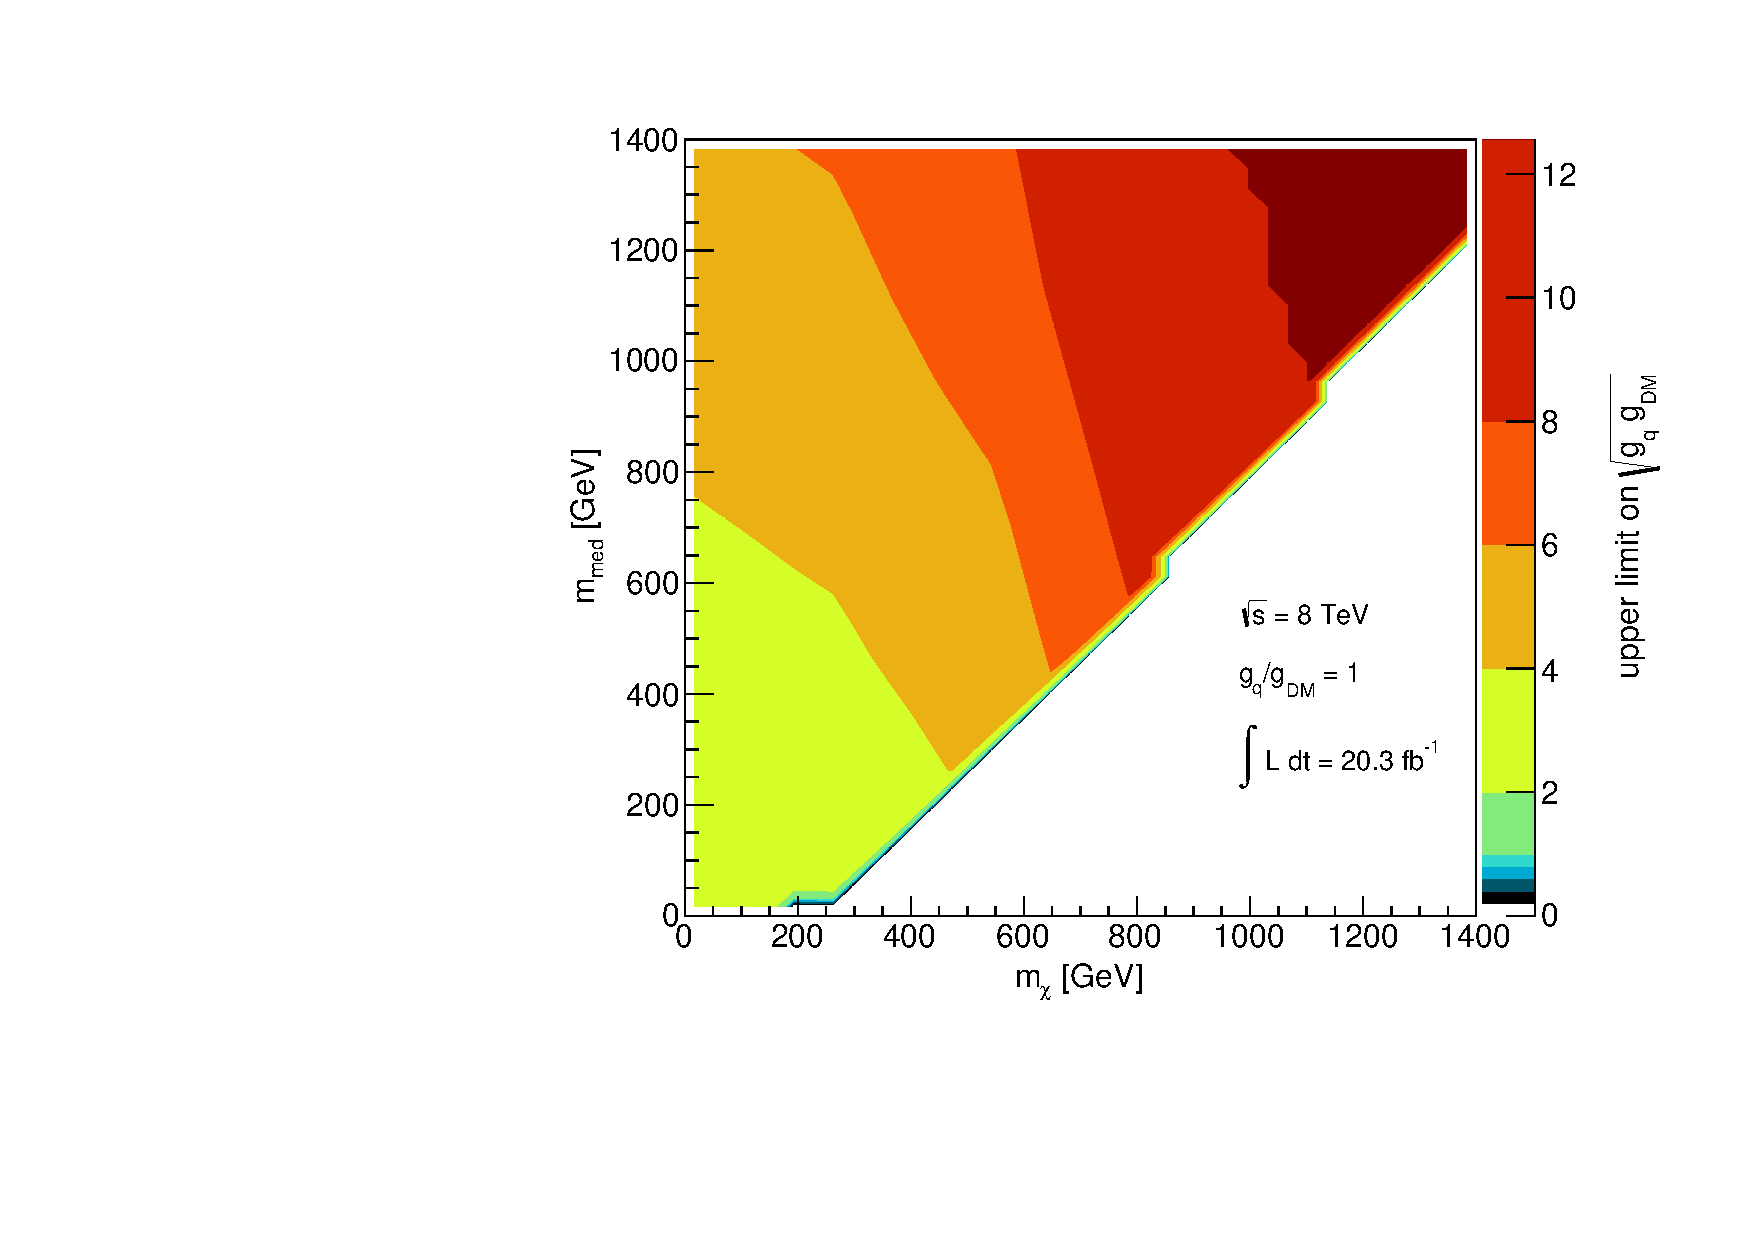
\includegraphics[width=0.45\textwidth]{figures/coupling_limits_TSD_1.pdf}
\caption{Limit on coupling strength for the sV model, in the mono-Z channel.  Need to fix up the scale on the z-axis and include mass points as dots on the plot. To be replaced with 5 plots with different coupling ratios, gq/gchi = 0.2, 0.5, 1, 2, 5. REPLACE WITH SV MODEL PLOTS.}
\label{fig:MonoZ_SVD_couplinglimit}
\end{center}
\end{figure}

\begin{figure}[!h]
\begin{center}
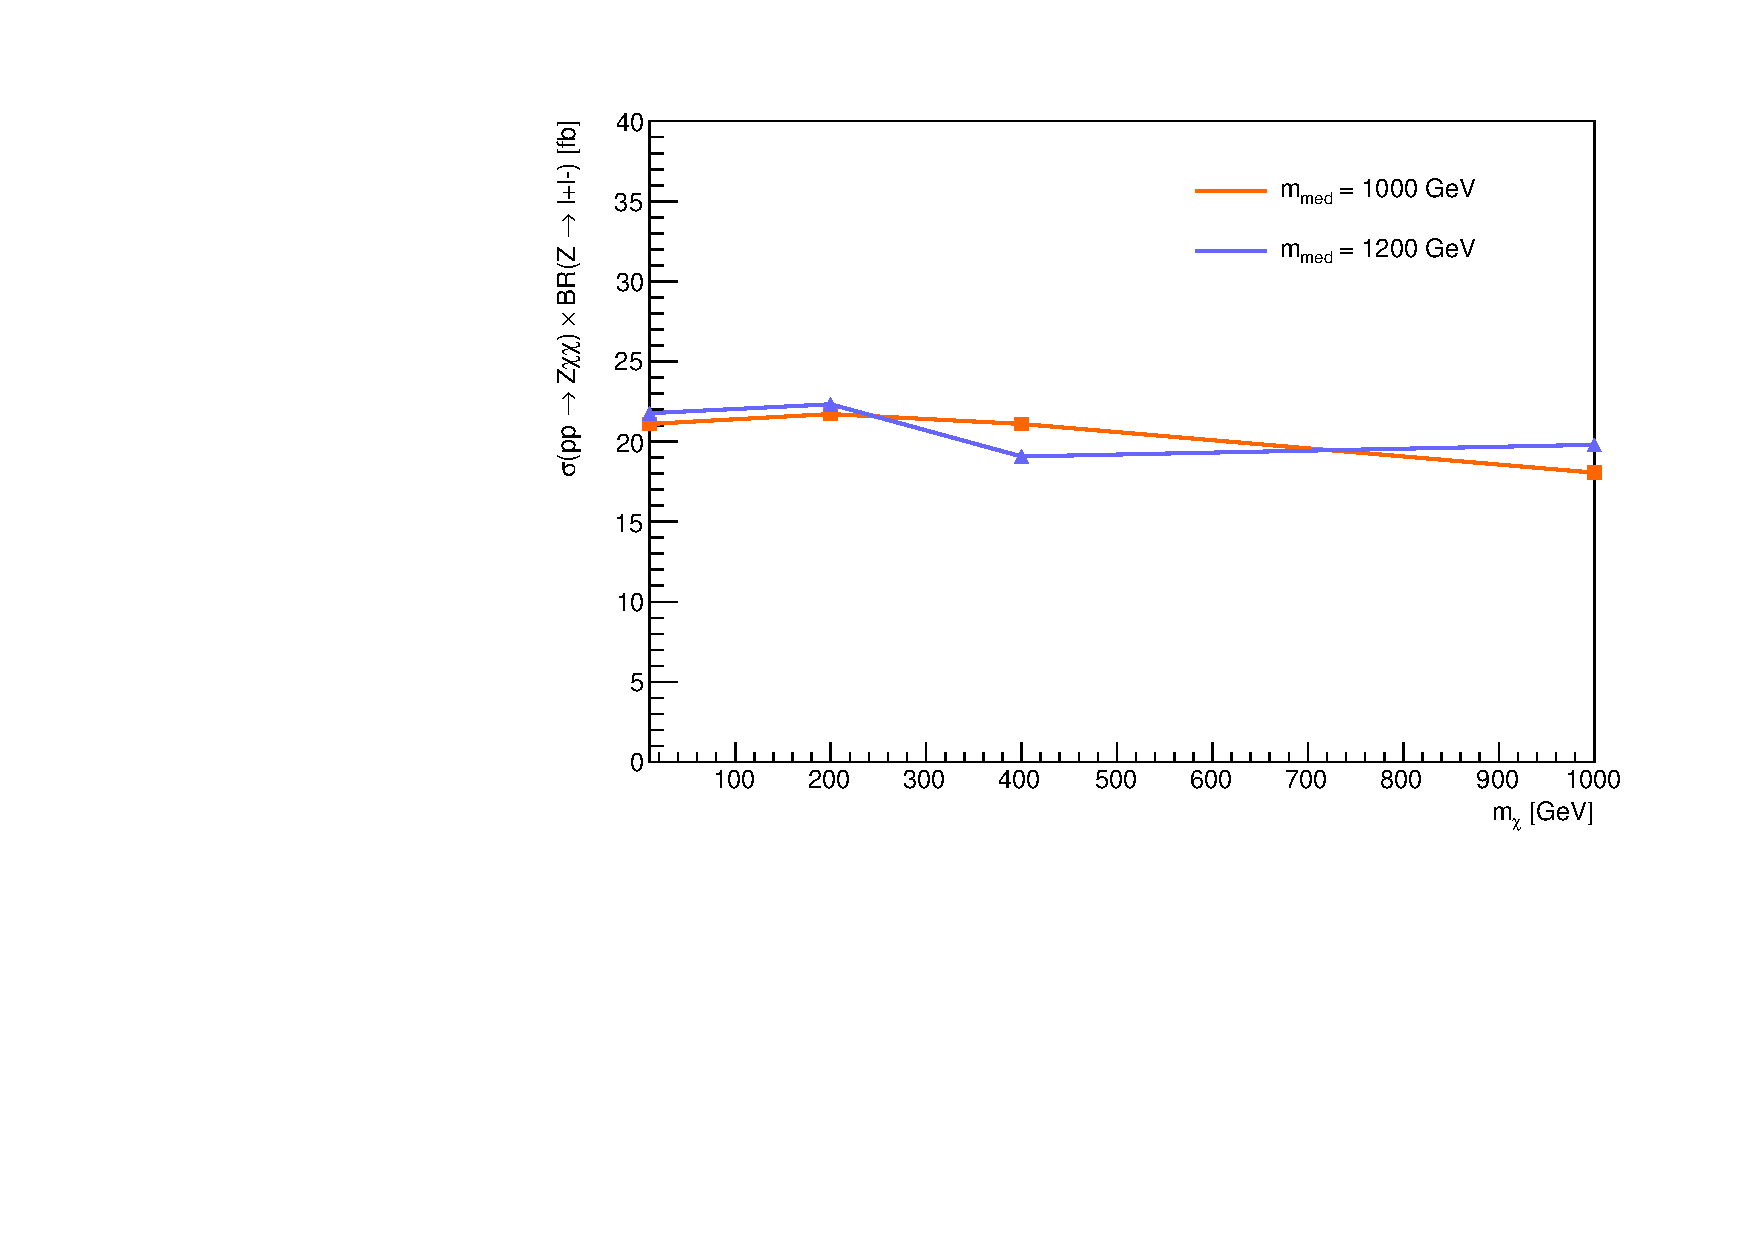
\includegraphics[width=0.45\textwidth]{figures/monoZ_sigma_limits_variedDMmass.pdf}
\caption{Mono-Z channel, sS model. REPLACE WITH SS MODEL PLOTS.}
\label{fig:MonoZ_SSD_limit}
\end{center}
\end{figure}

\begin{figure}[!h]
\begin{center}
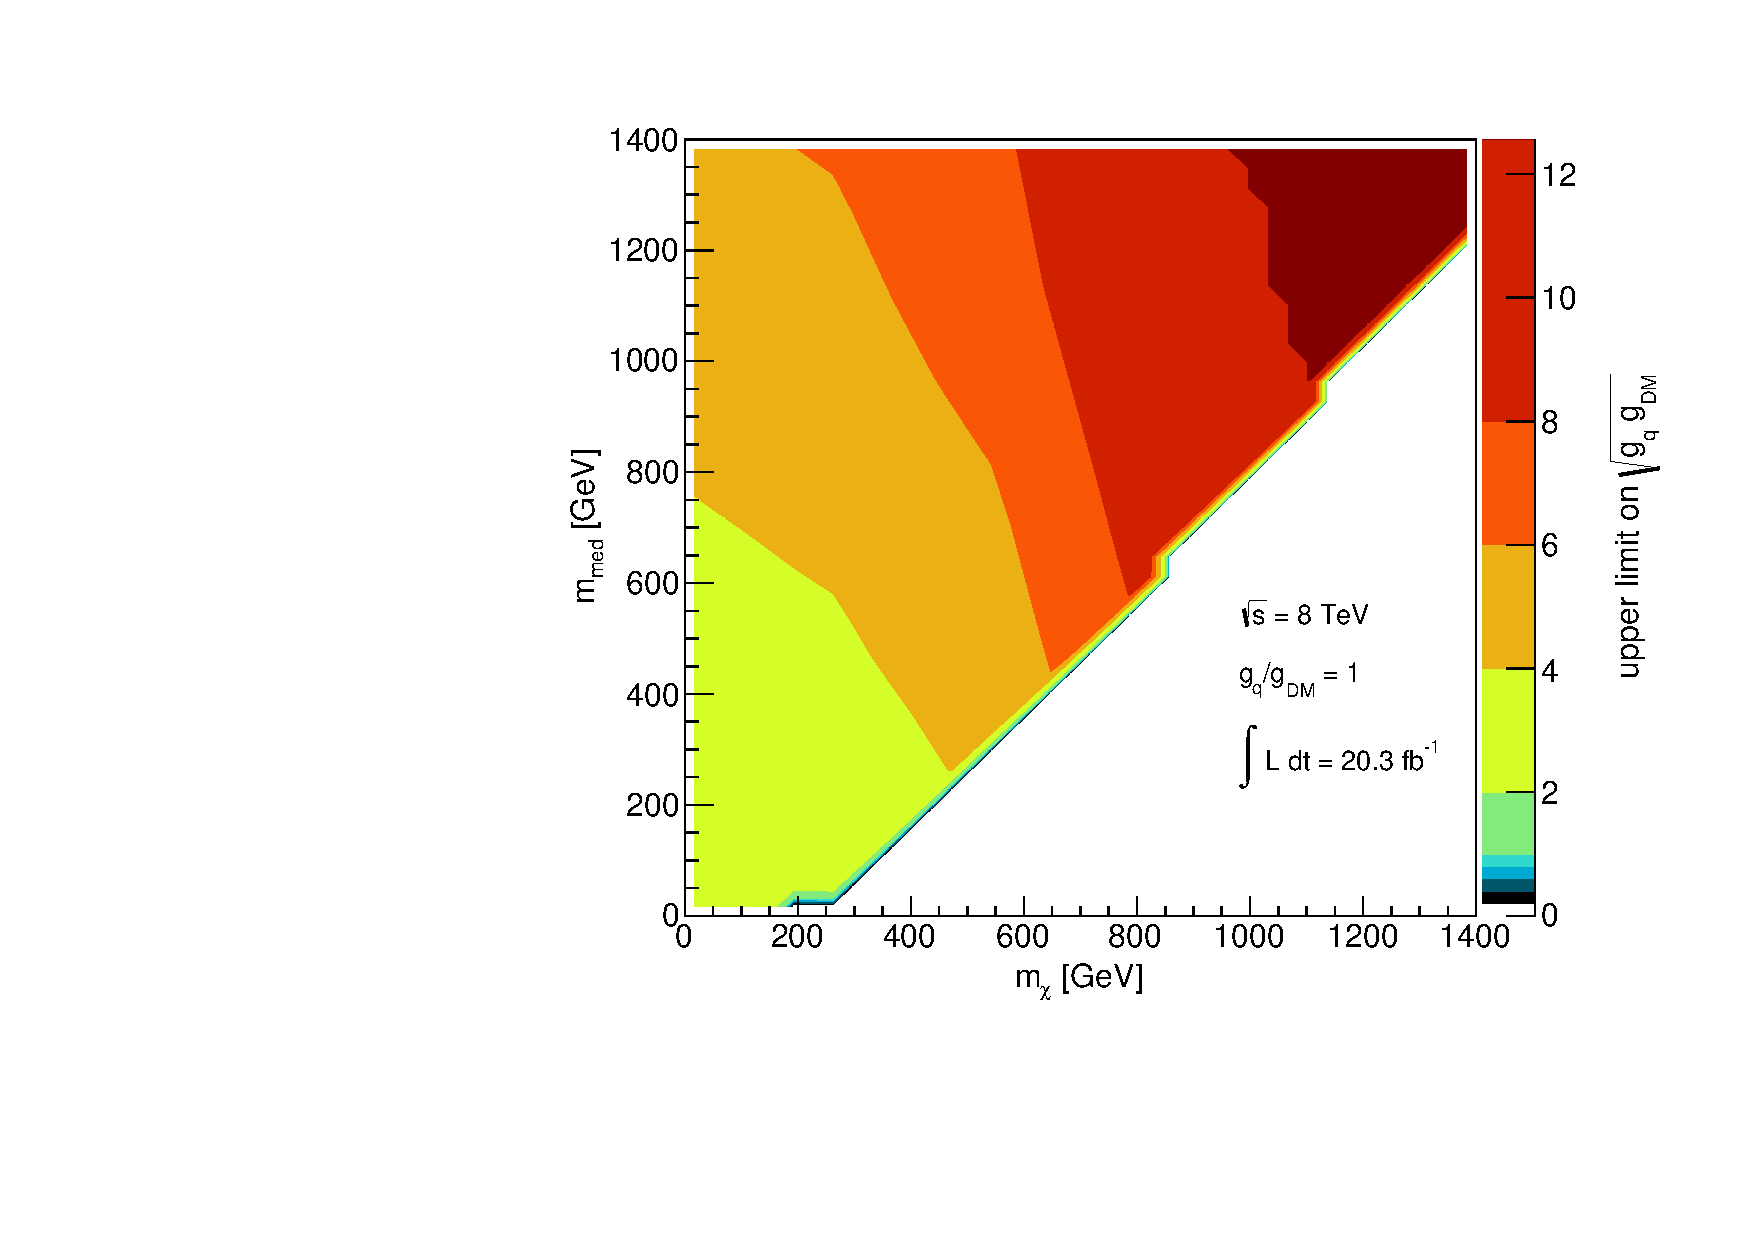
\includegraphics[width=0.45\textwidth]{figures/coupling_limits_TSD_1.pdf}
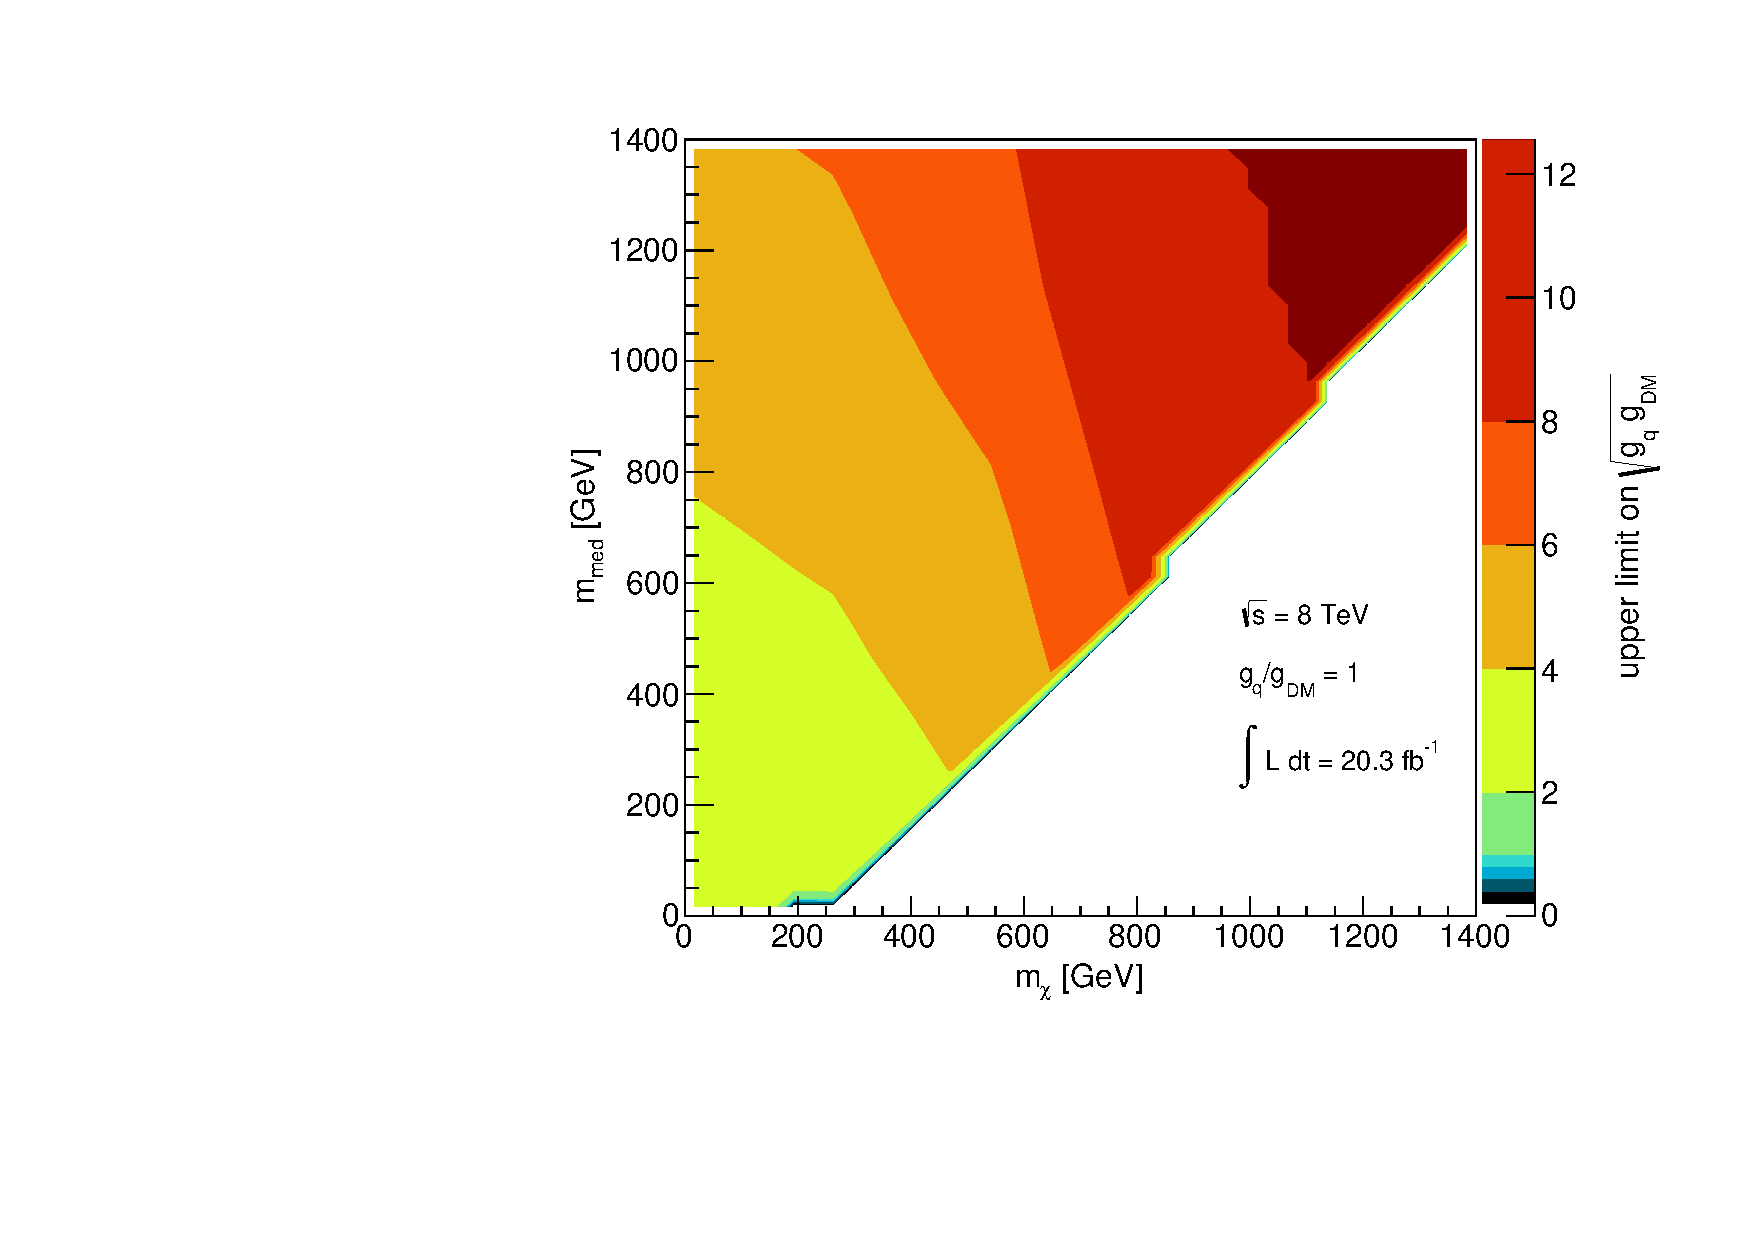
\includegraphics[width=0.45\textwidth]{figures/coupling_limits_TSD_1.pdf}
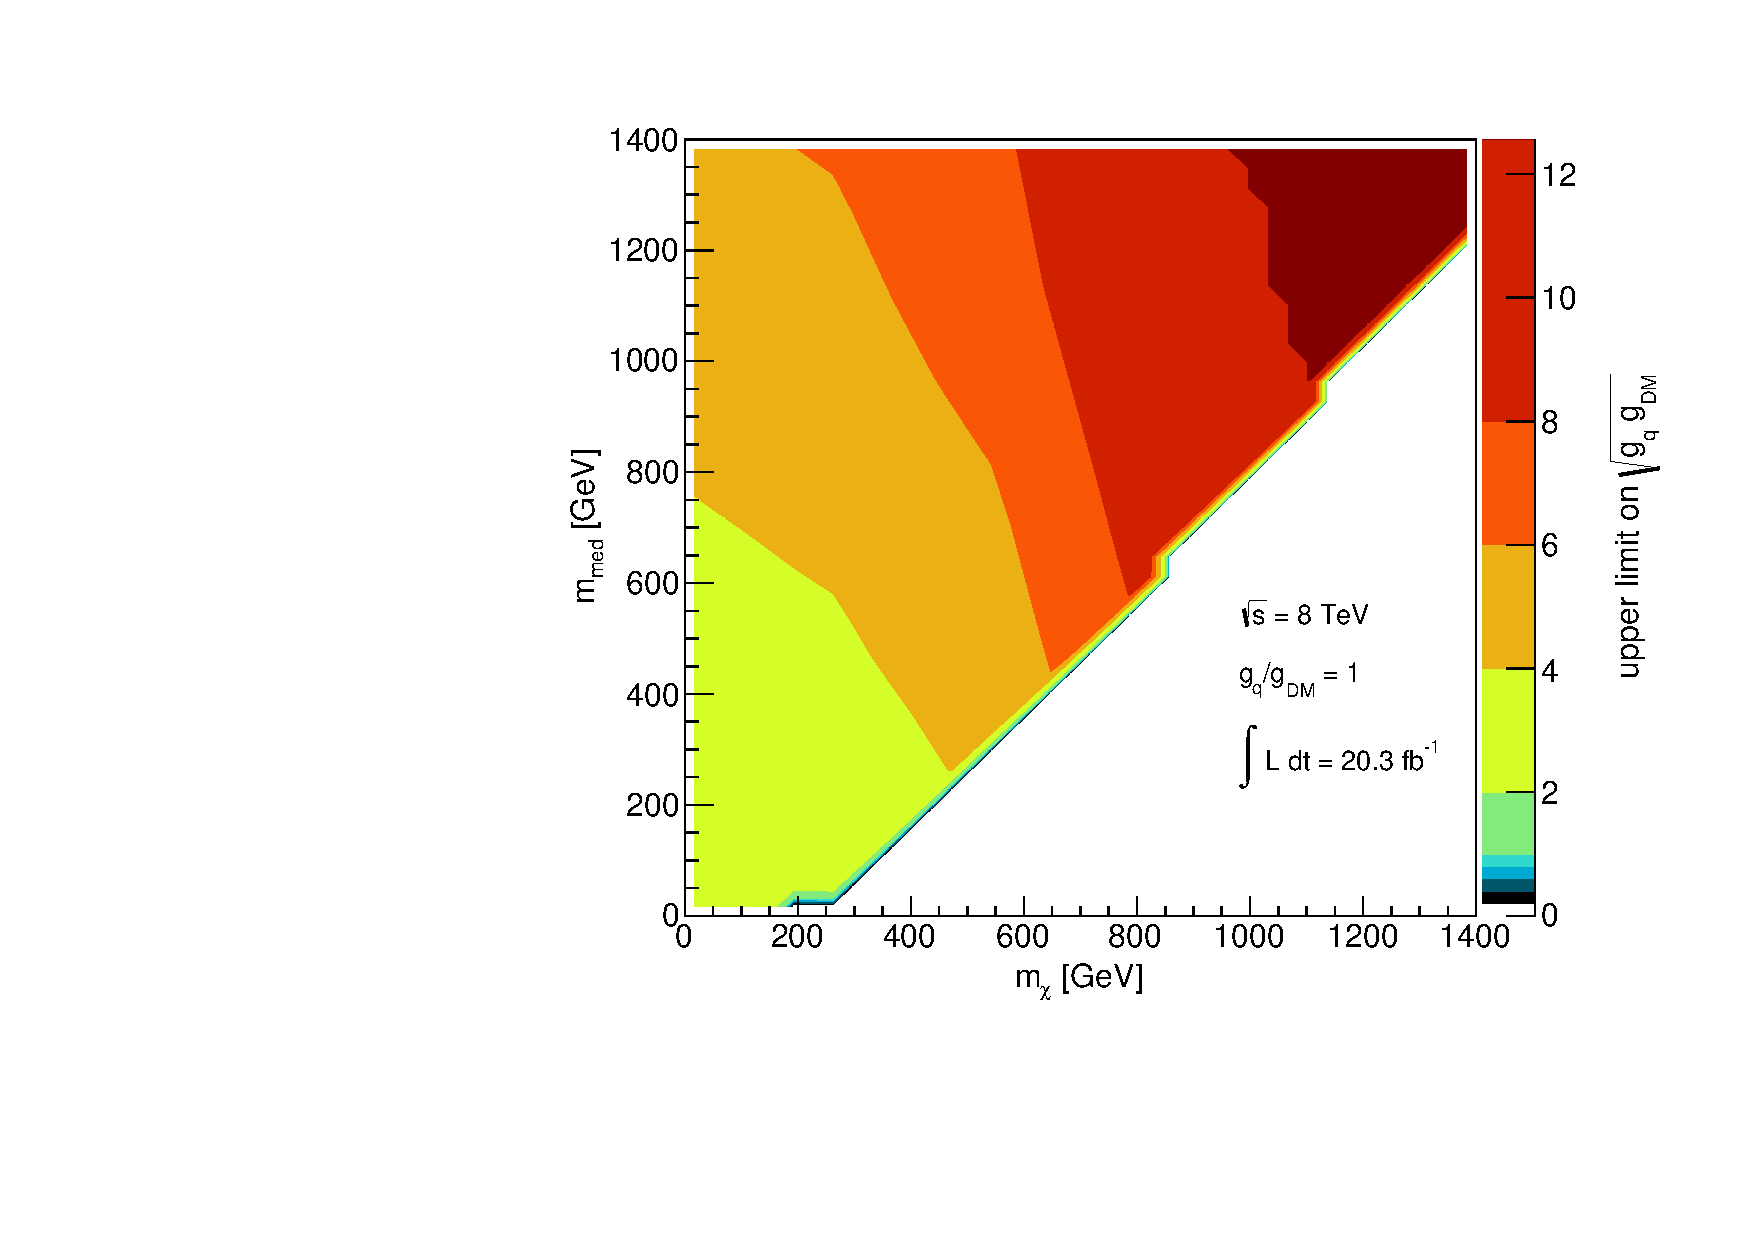
\includegraphics[width=0.45\textwidth]{figures/coupling_limits_TSD_1.pdf}
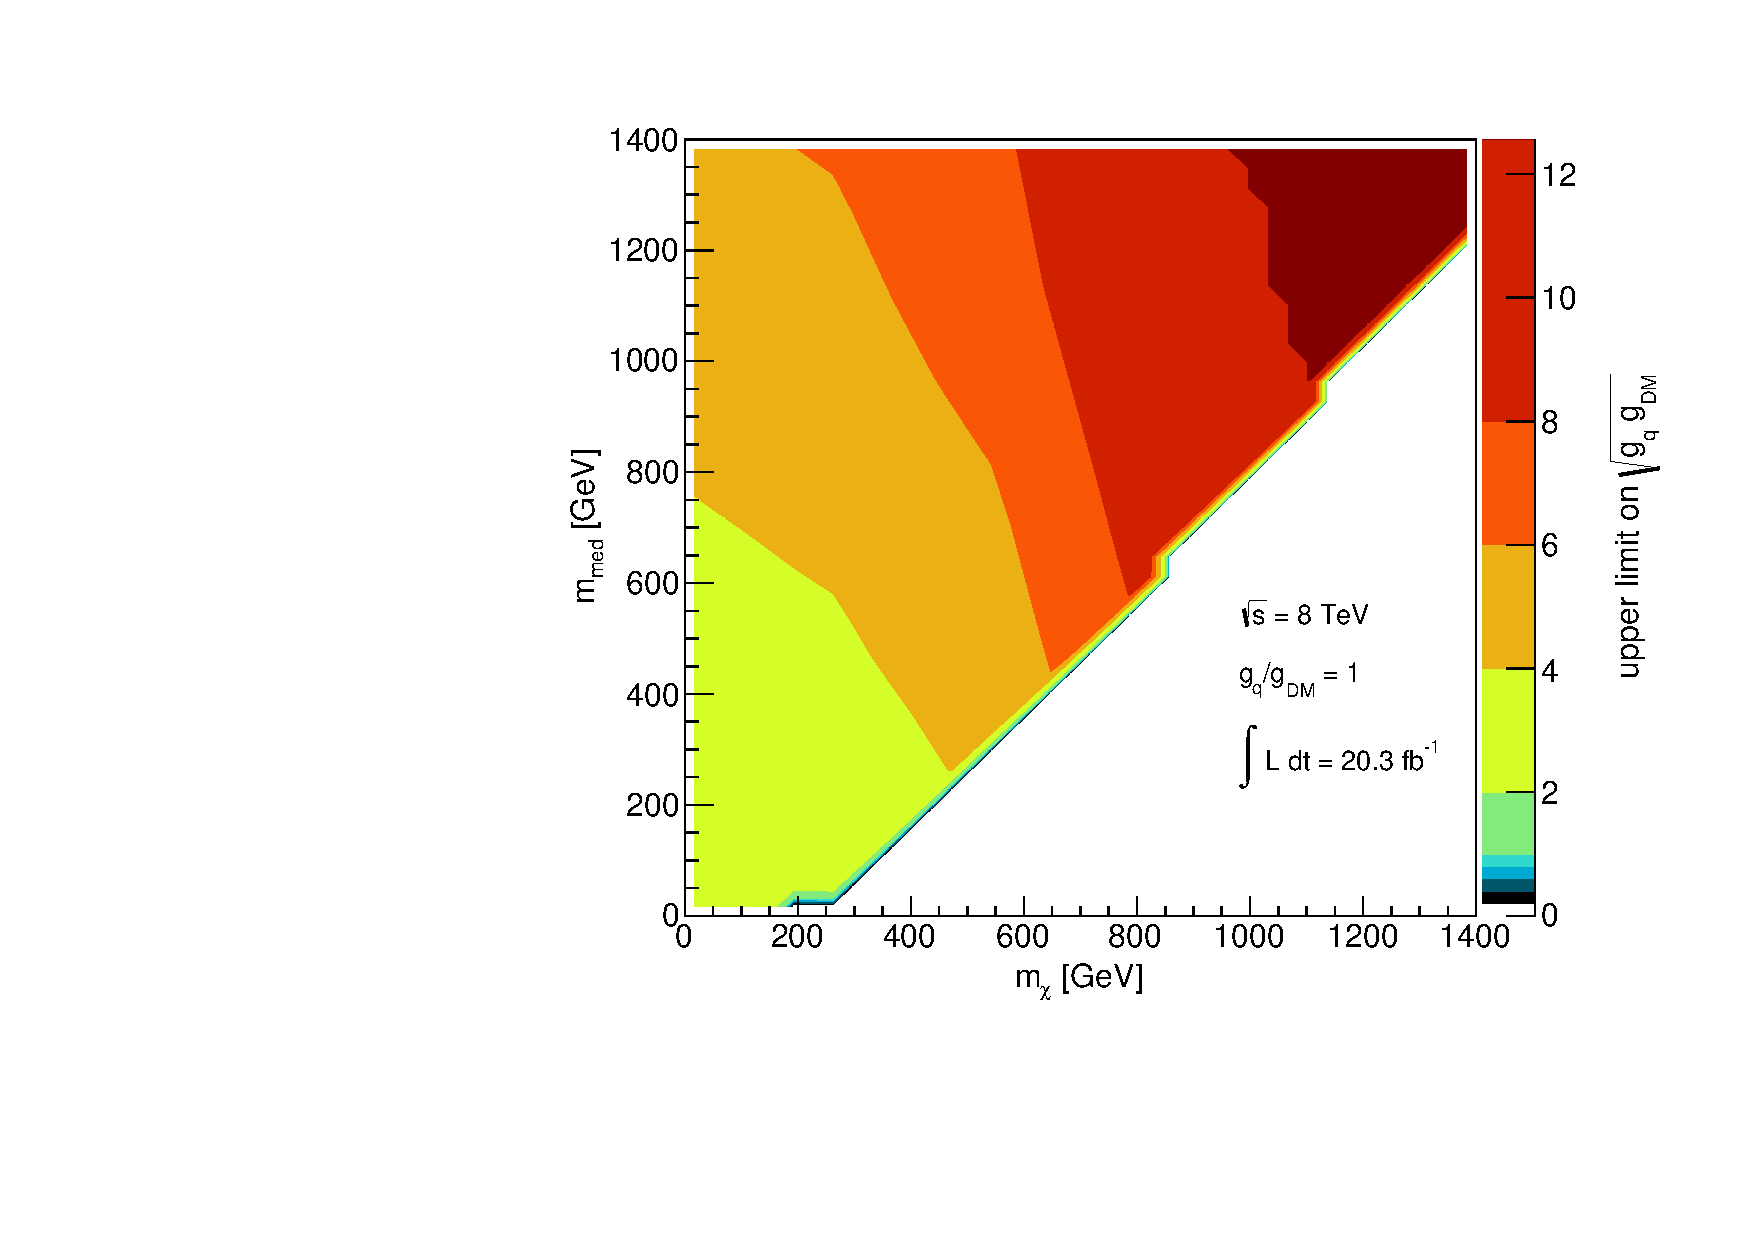
\includegraphics[width=0.45\textwidth]{figures/coupling_limits_TSD_1.pdf}
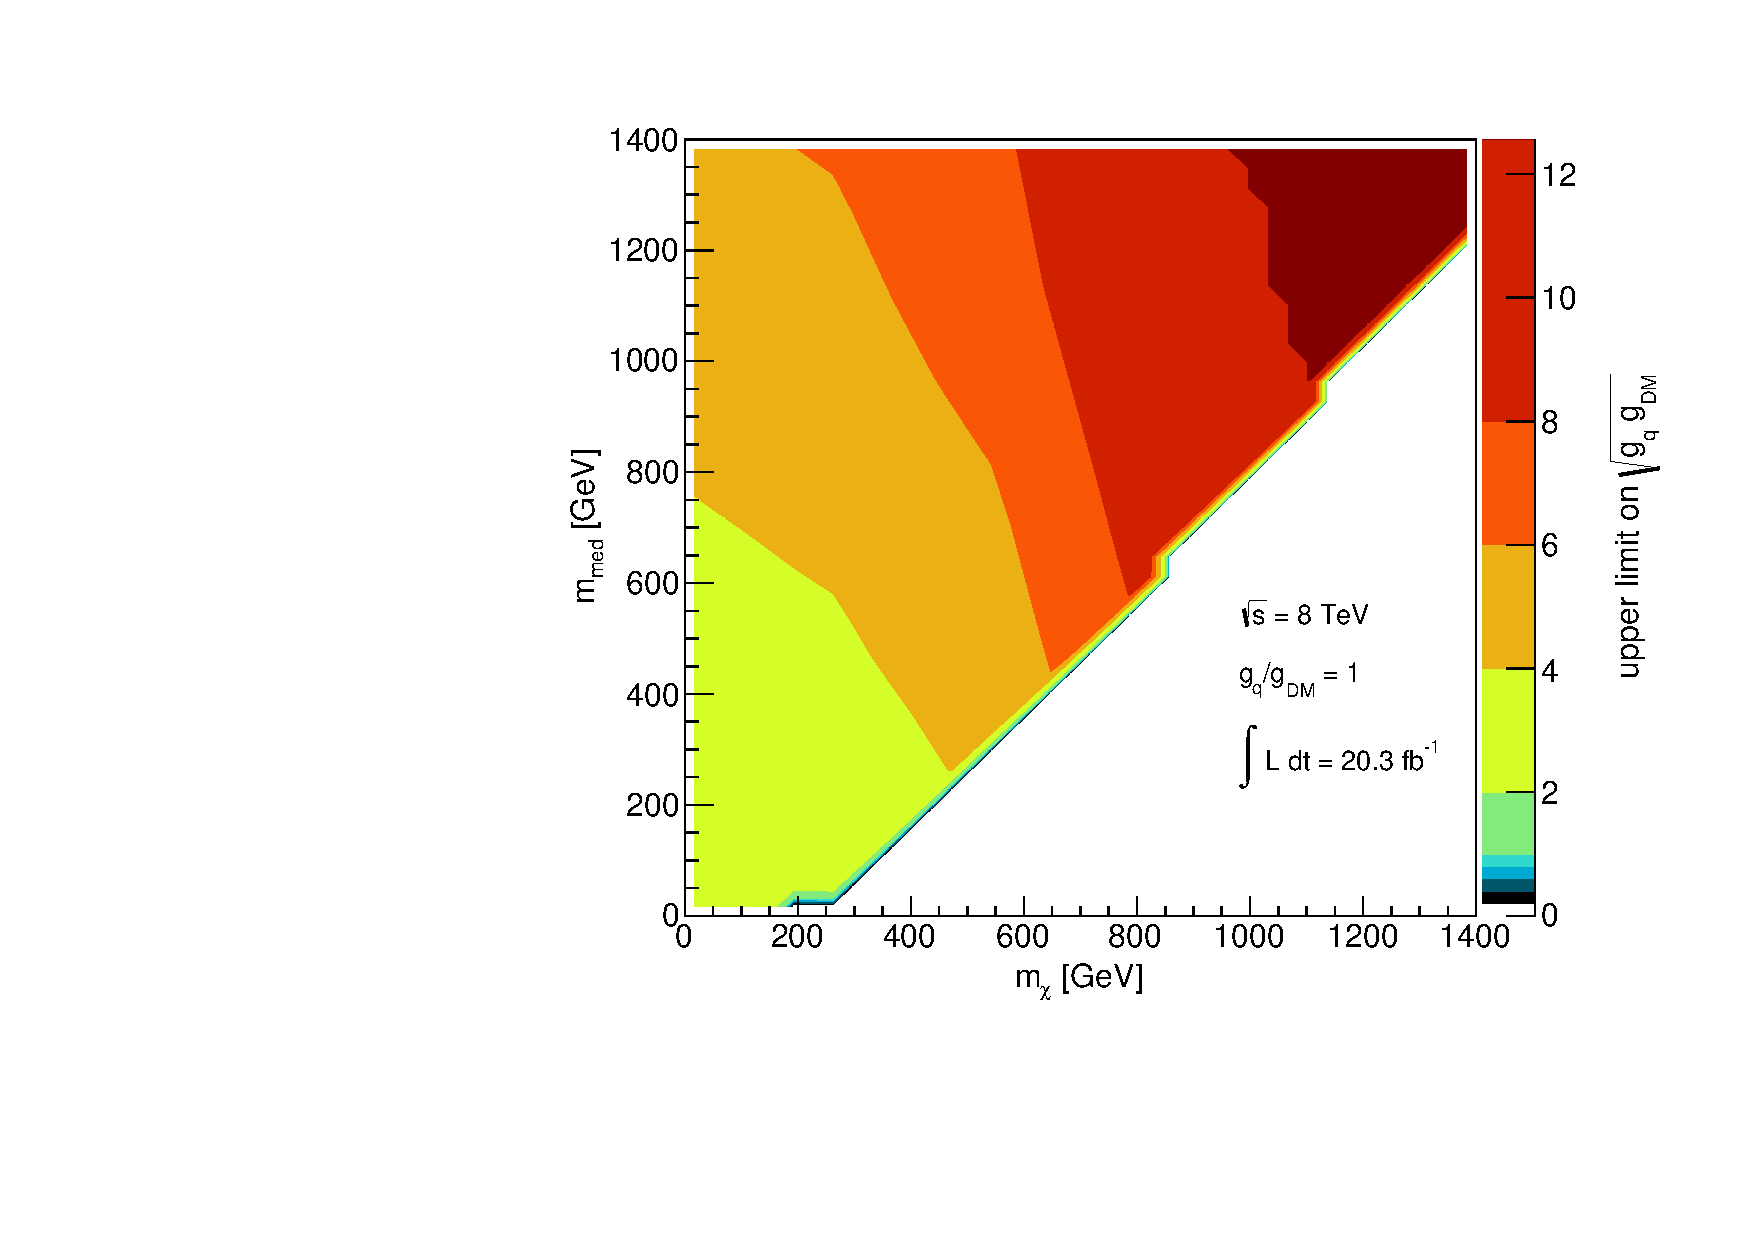
\includegraphics[width=0.45\textwidth]{figures/coupling_limits_TSD_1.pdf}
\caption{sS model coupling limit. REPLACE WITH SS MODEL PLOTS.}
\label{fig:MonoZ_SSD_couplinglimit}
\end{center}
\end{figure}

\begin{figure}[!h]
\begin{center}
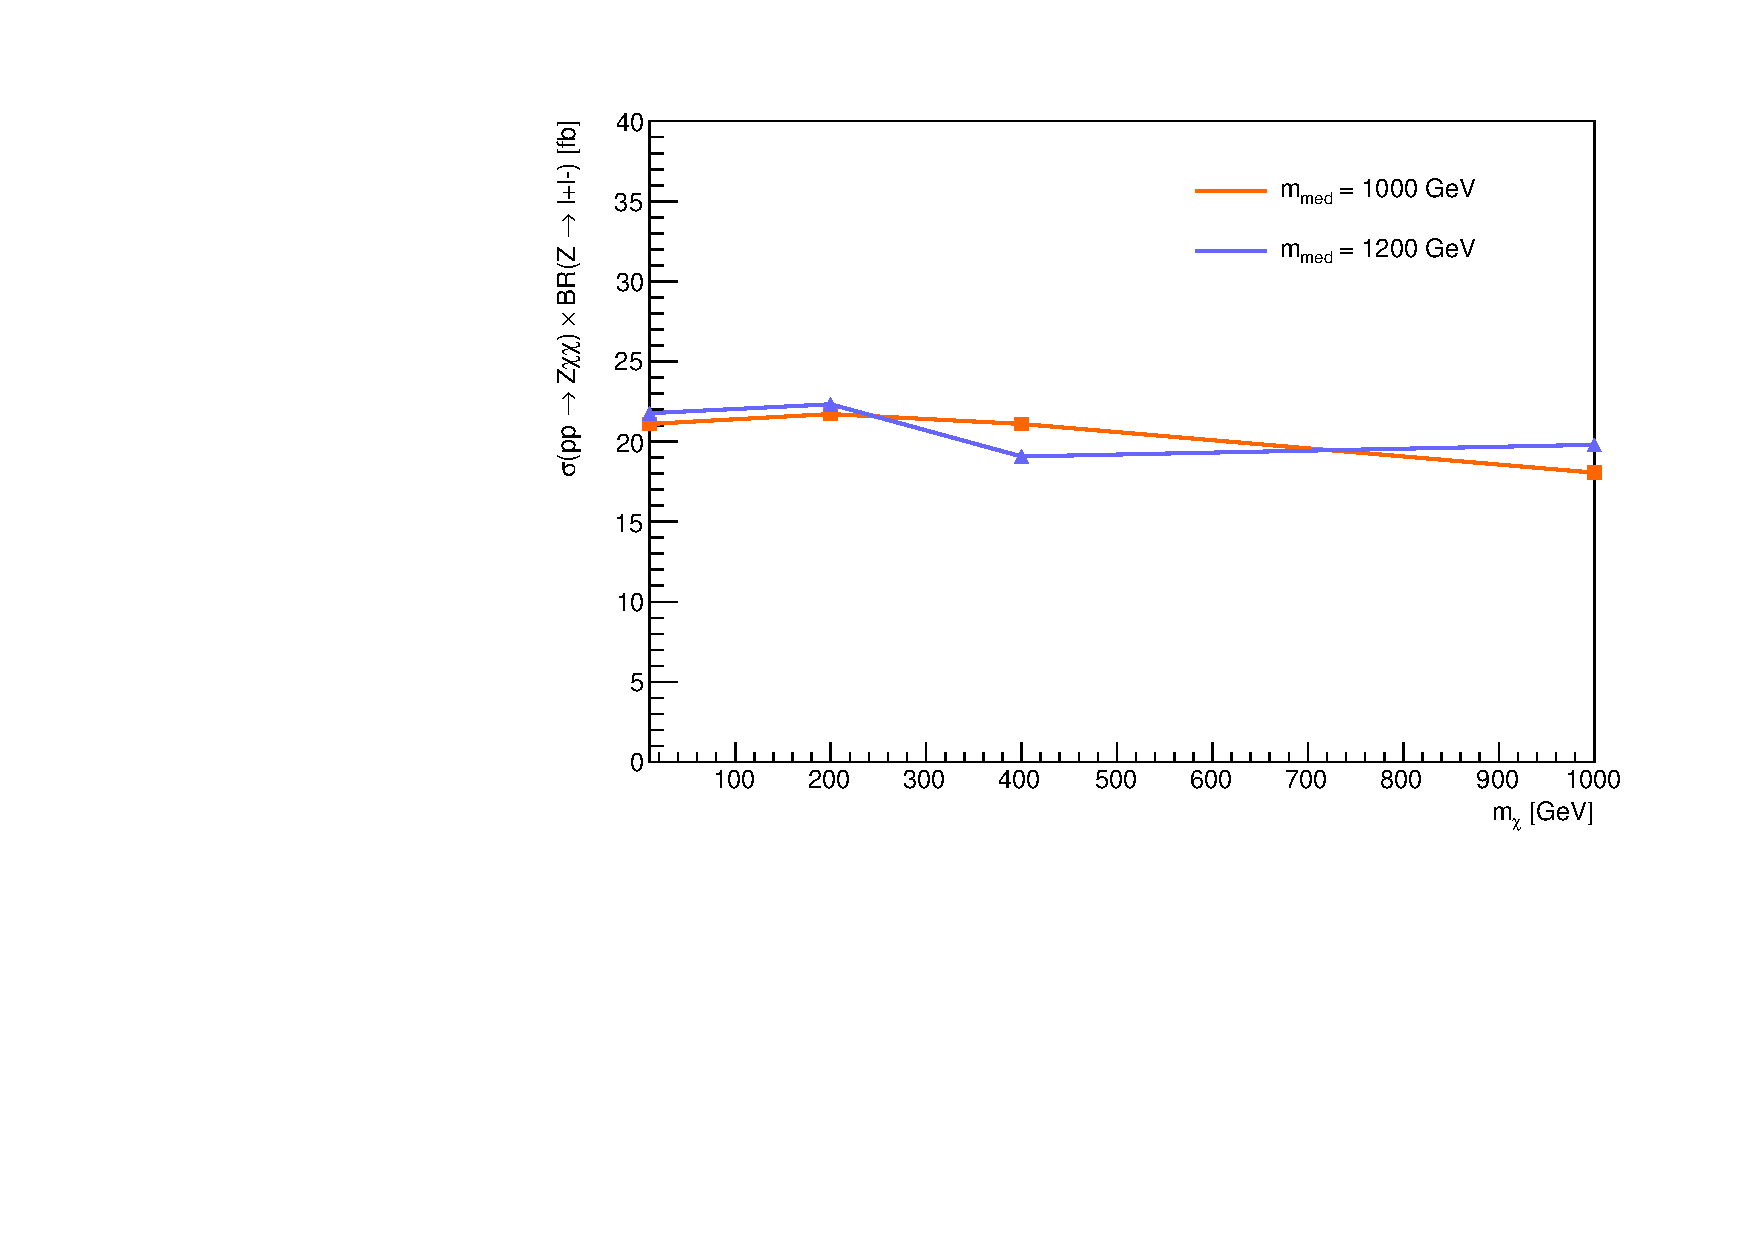
\includegraphics[width=0.45\textwidth]{figures/monoZ_sigma_limits_variedDMmass.pdf}
\caption{Mono-Z channel, tS model. REPLACE WITH TS MODEL PLOTS.}
\label{fig:MonoZ_TSD_limit}
\end{center}
\end{figure}

\begin{figure}[!h]
\begin{center}
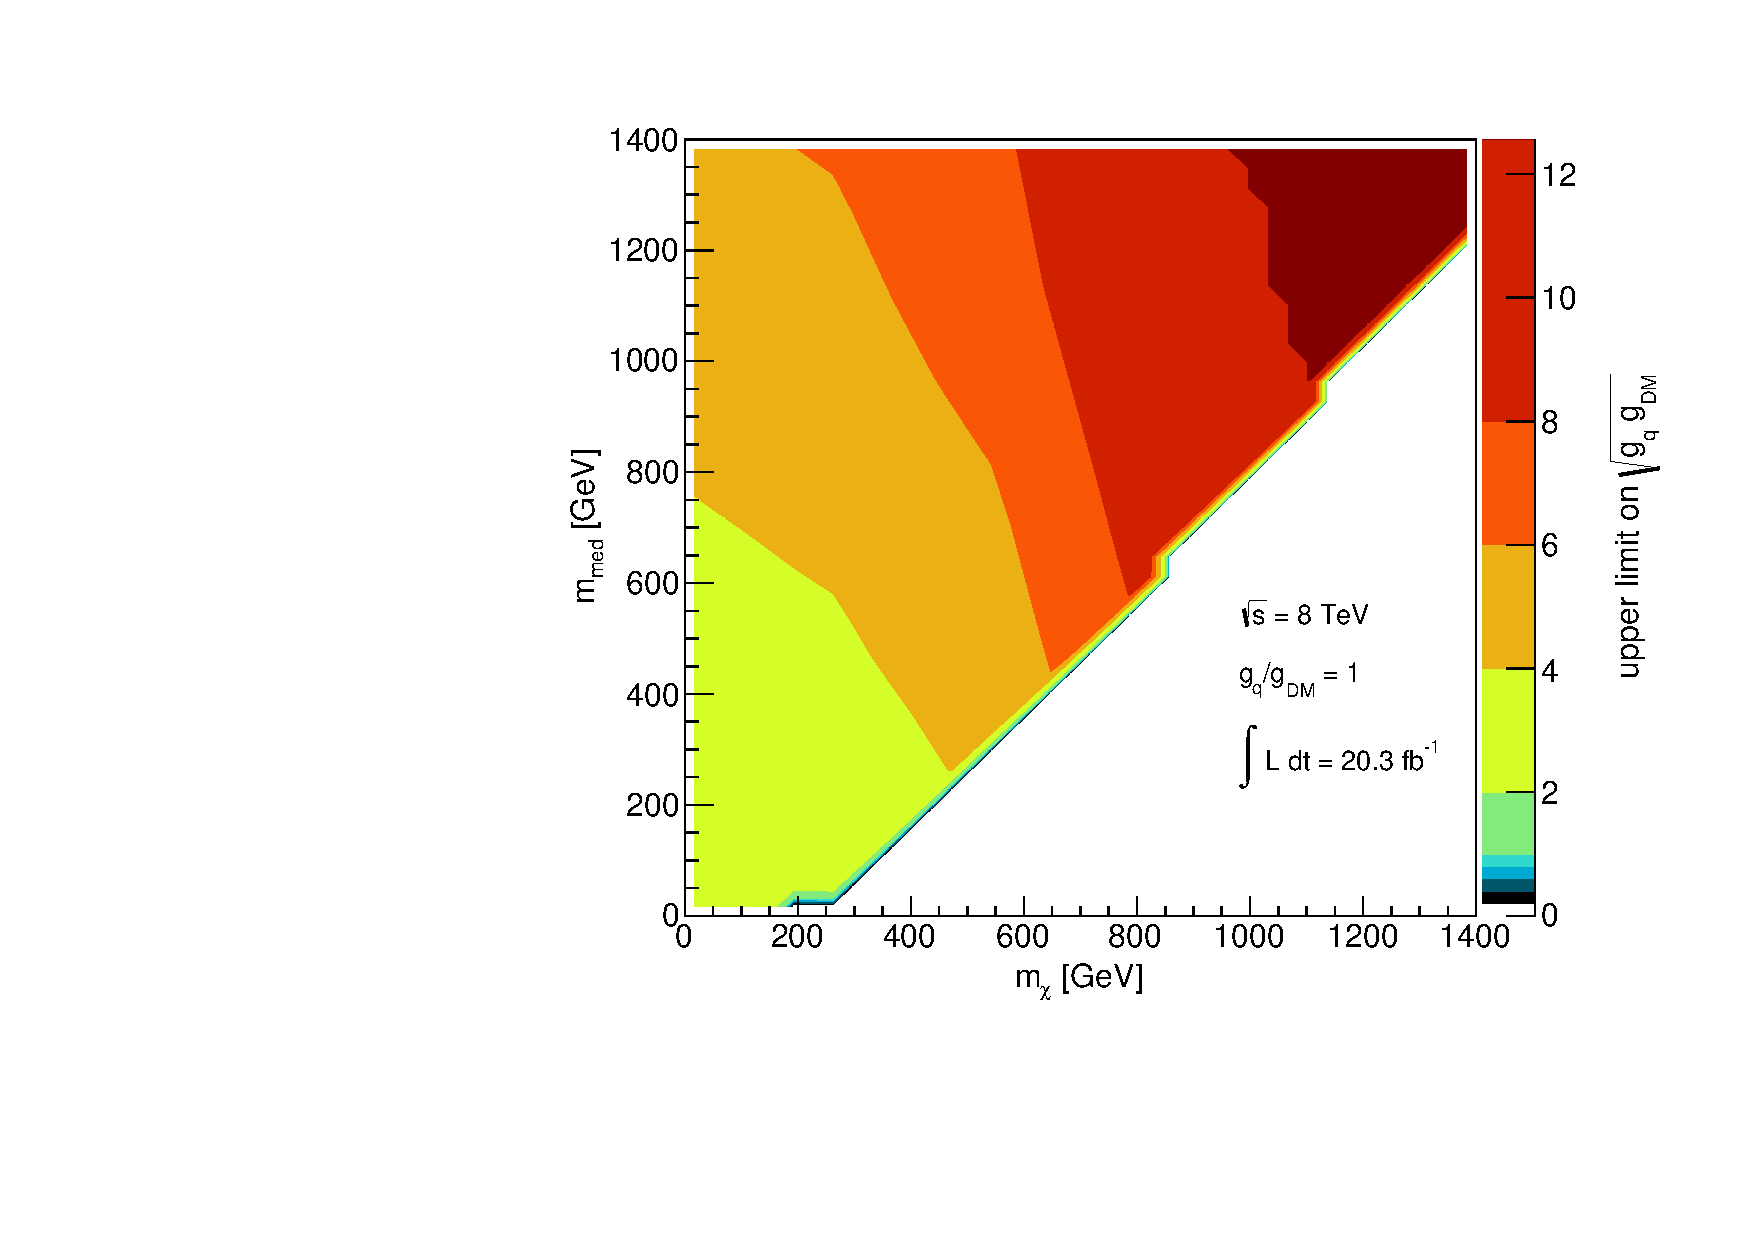
\includegraphics[width=0.45\textwidth]{figures/coupling_limits_TSD_1.pdf}
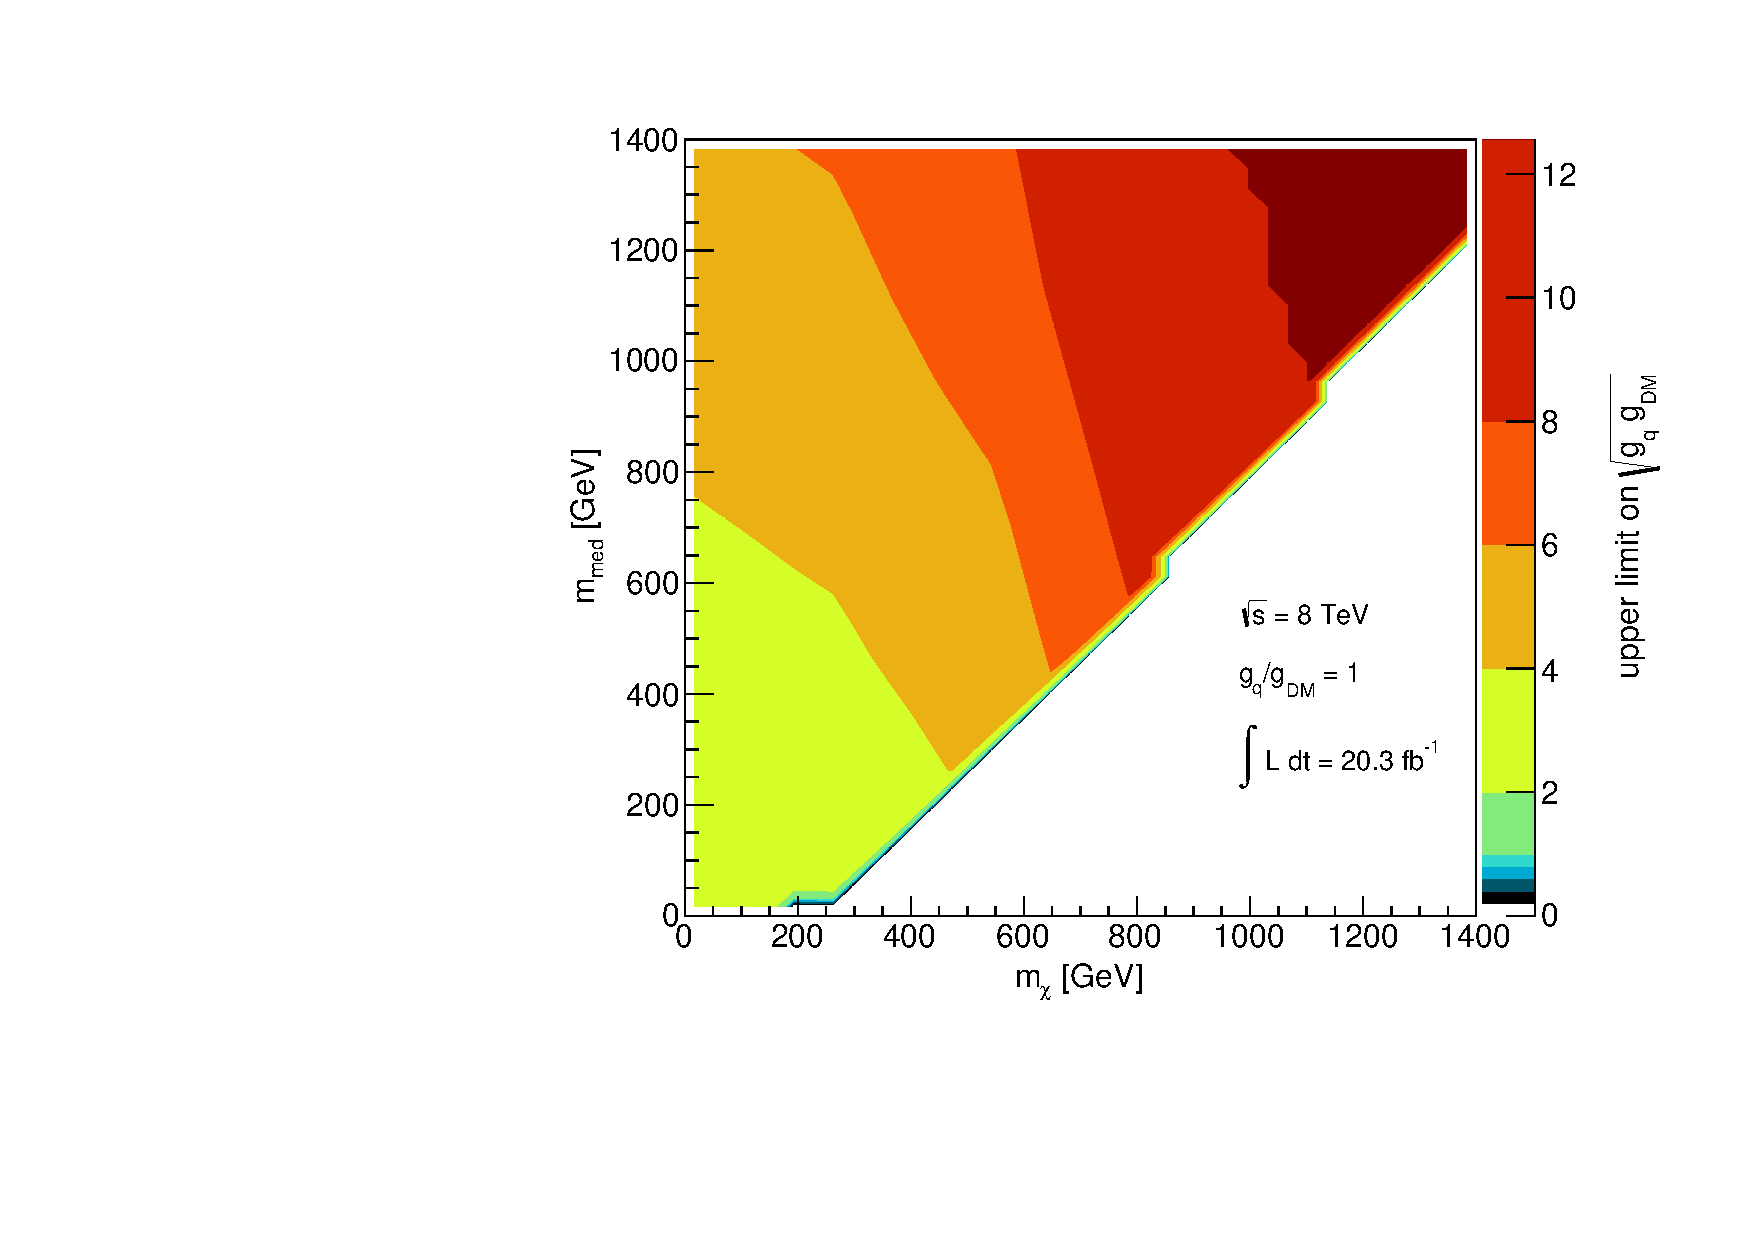
\includegraphics[width=0.45\textwidth]{figures/coupling_limits_TSD_1.pdf}
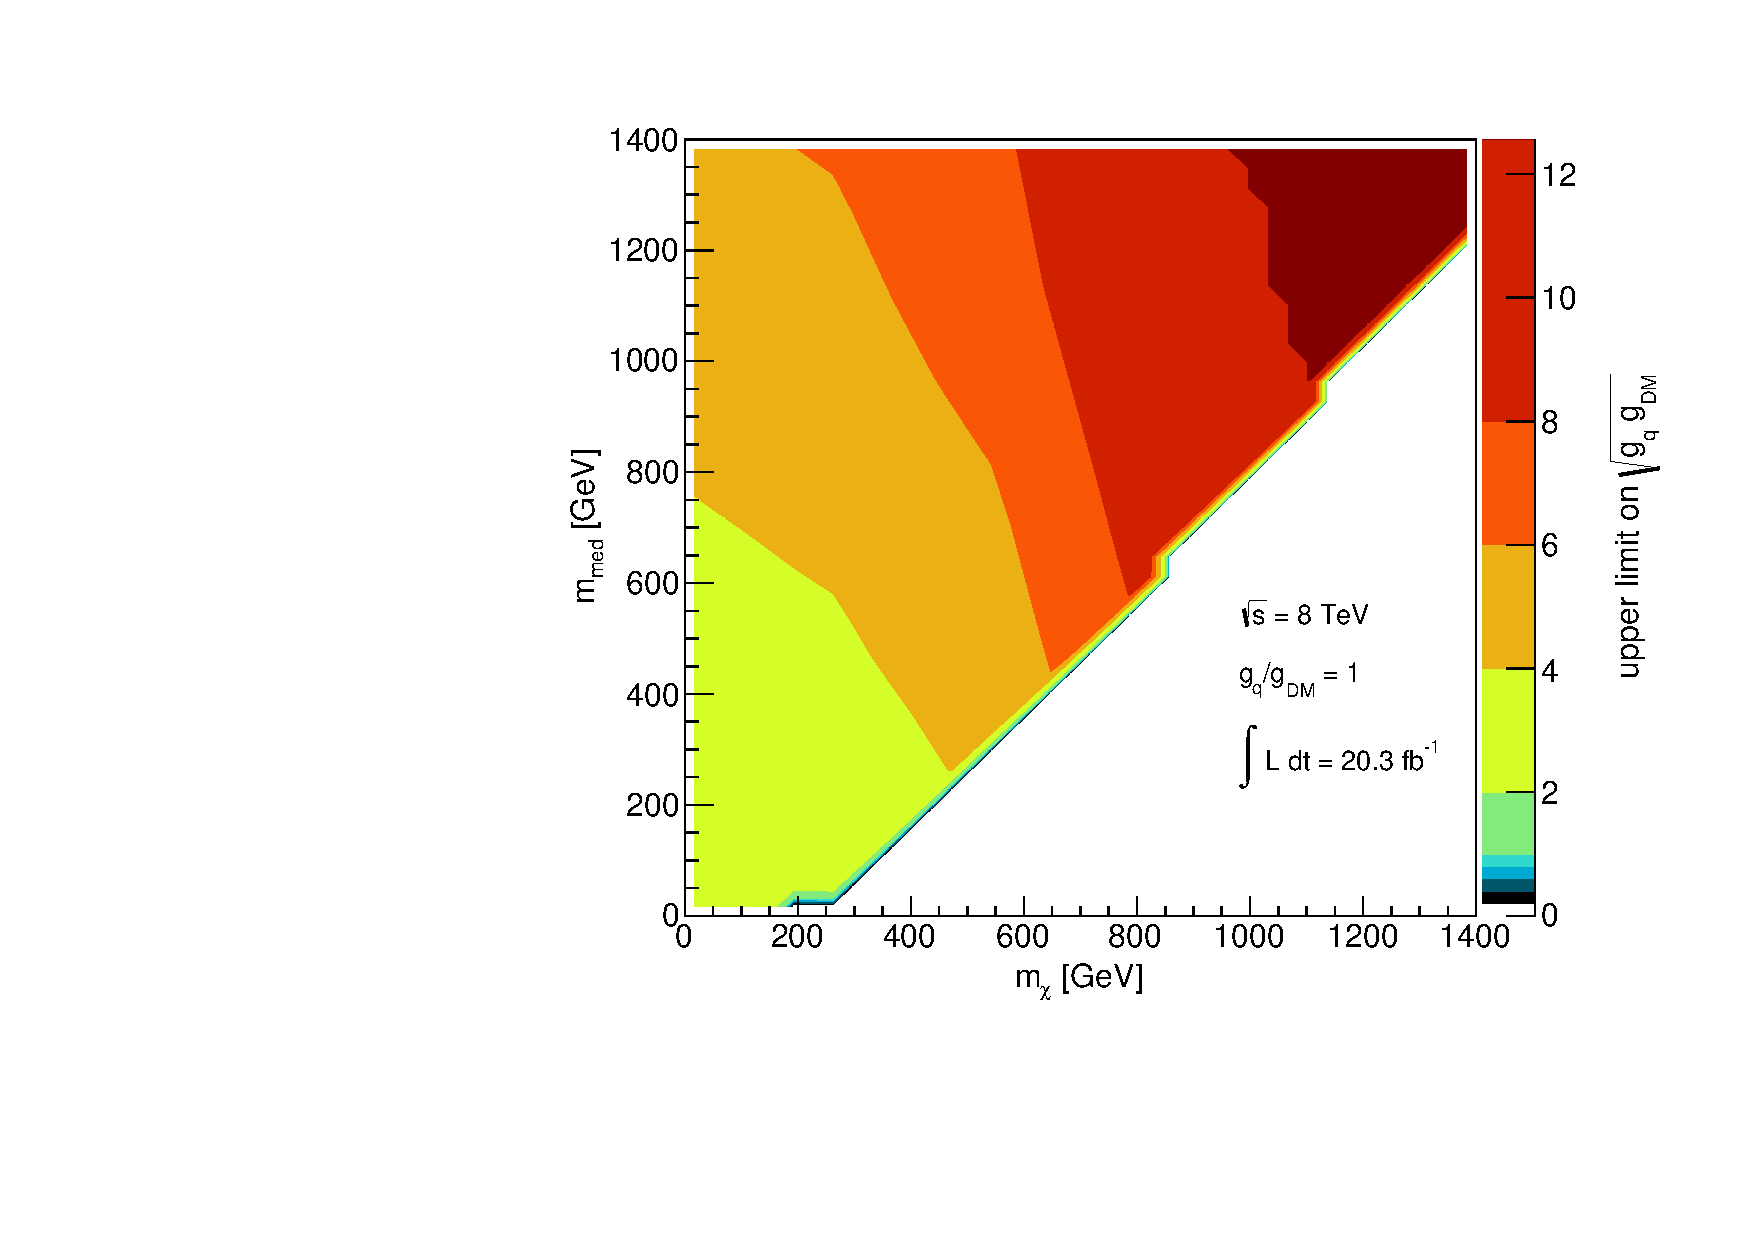
\includegraphics[width=0.45\textwidth]{figures/coupling_limits_TSD_1.pdf}
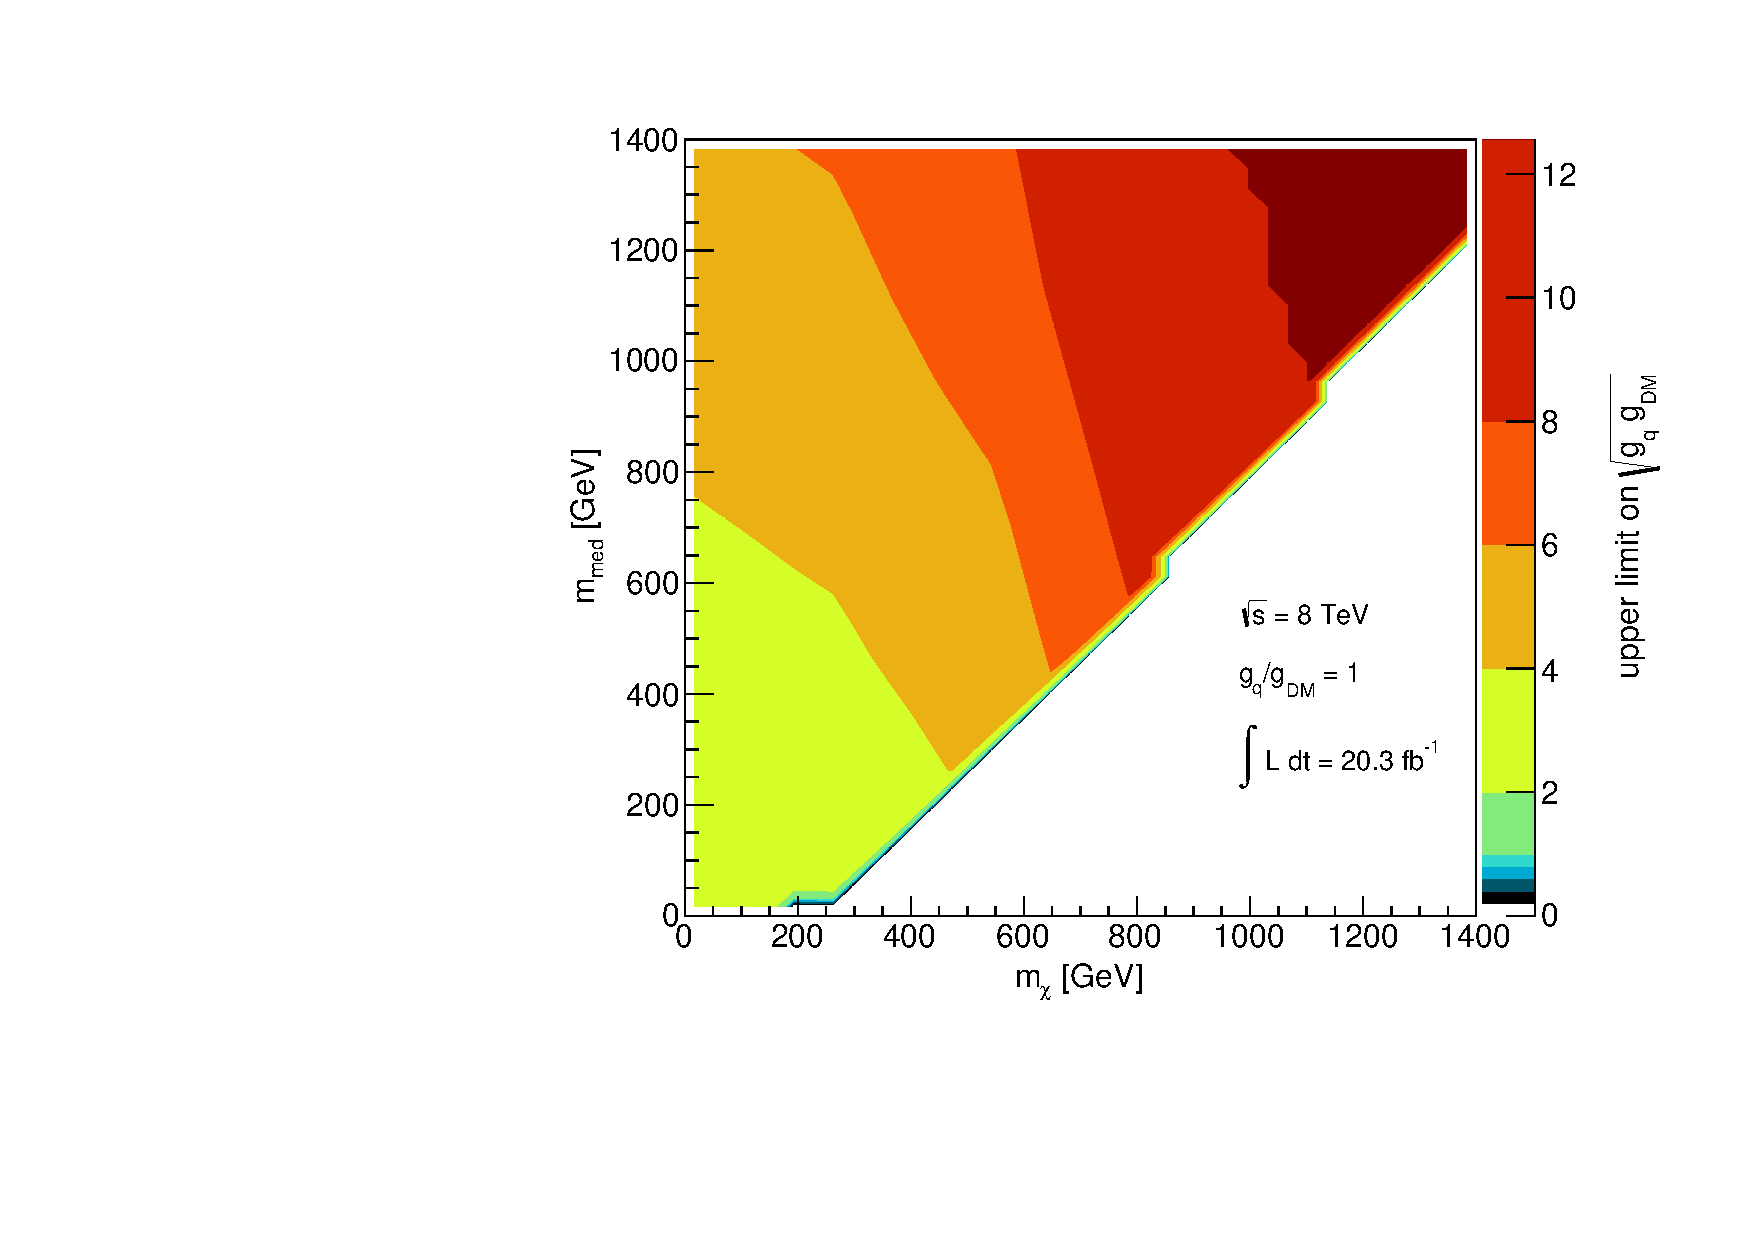
\includegraphics[width=0.45\textwidth]{figures/coupling_limits_TSD_1.pdf}
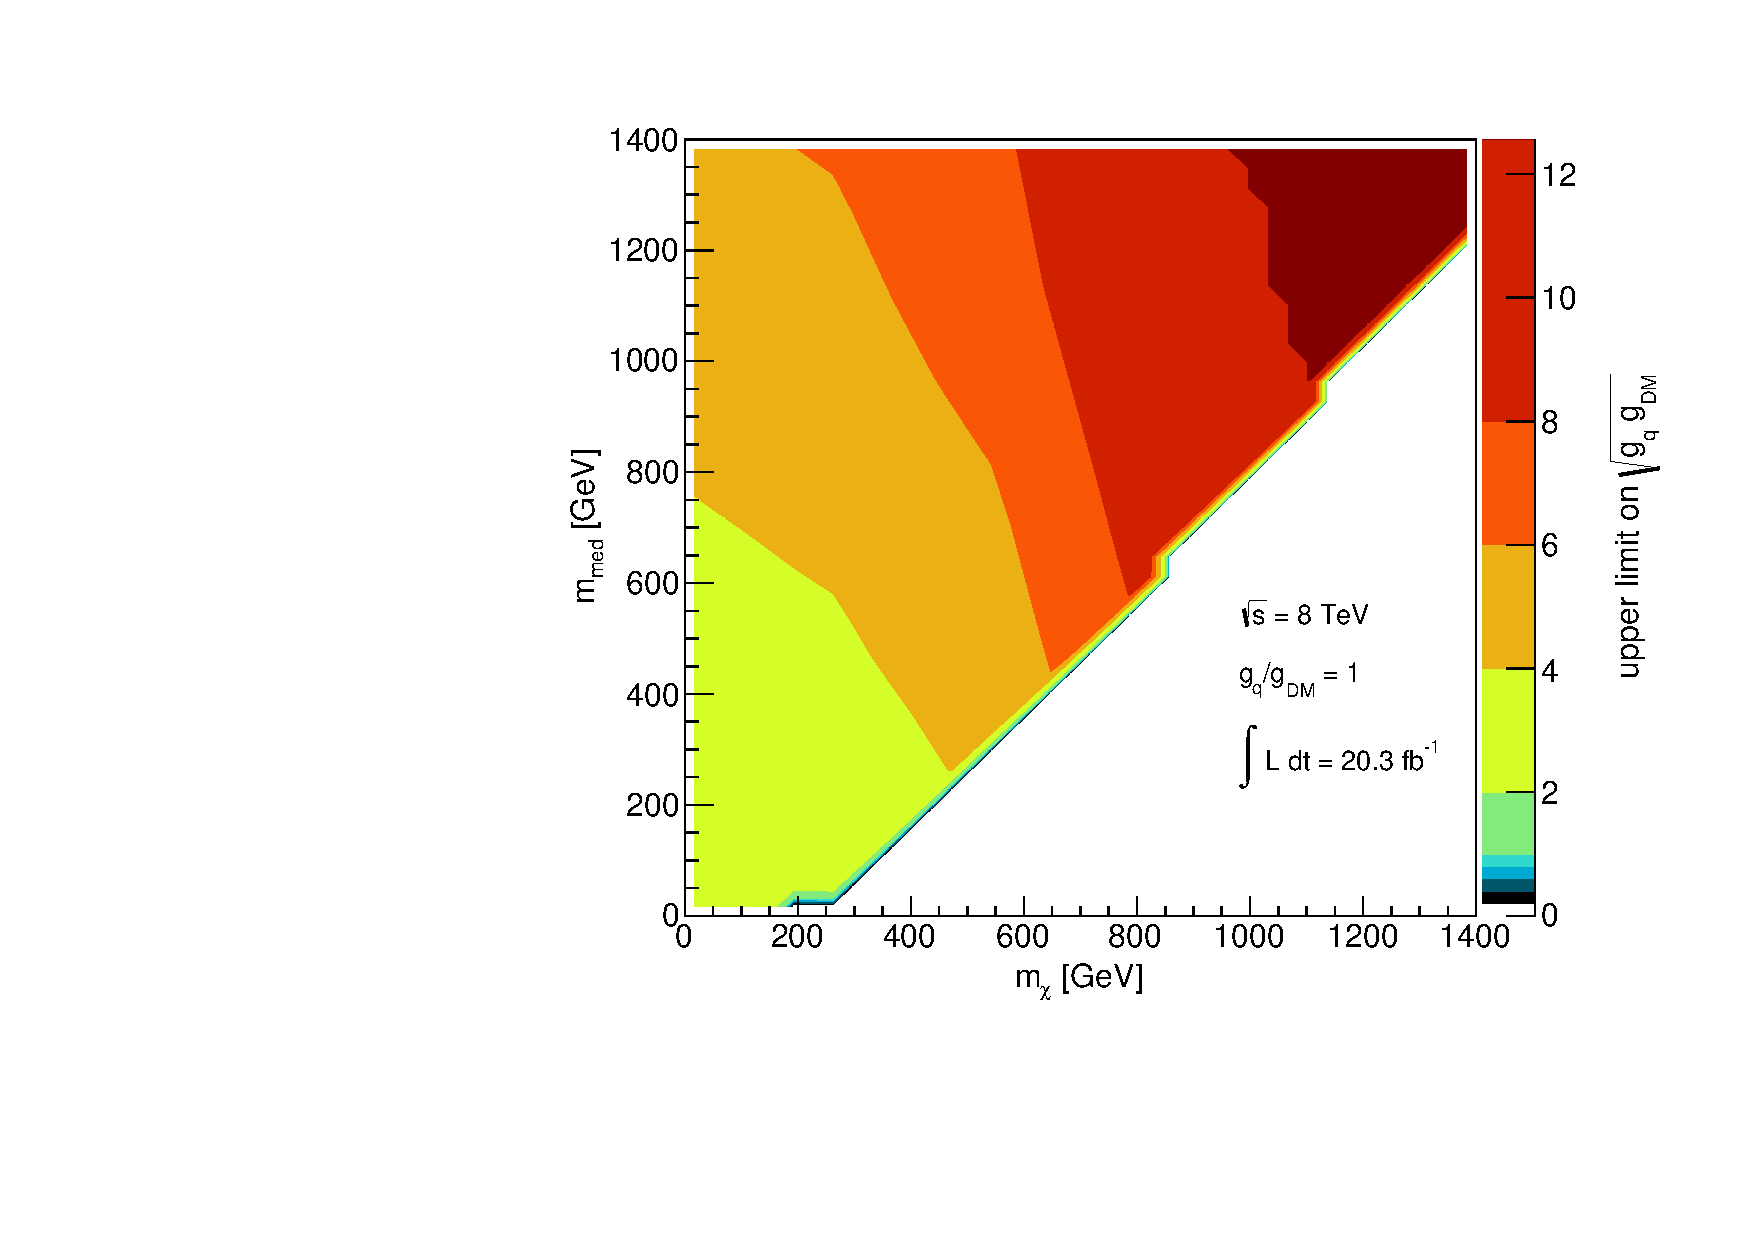
\includegraphics[width=0.45\textwidth]{figures/coupling_limits_TSD_1.pdf}
\caption{tS model coupling limit. REPLACE WITH TS MODEL PLOTS.}
\label{fig:MonoZ_TSD_couplinglimit}
\end{center}
\end{figure}

%%%%%%%%%%%%%%%%%%%%%%%%%%%%%%%%
\subsection{Comparison with Relic Density Constraints}
%%%%%%%%%%%%%%%%%%%%%%%%%%%%%%%%

\comm{Copied from my paper with Karl, so I'll have to rewrite - Tom.}

If dark matter was produced thermally in the early universe, there is a simple relationship between the thermally averaged dark matter self-annihilation cross section $\langle\sigma v\rangle_{\rm ann}$, and the observed relic abundance $\Omega_{\rm DM}h^2$. For a given model, this allows us to find the coupling strength which provides the correct relic abundance as a function of $(m_\chi, M)$. 
%
This scenario is by no means a certainty; If the observed dark matter was produced through some mechanism other than thermal production, or if some new physics has an effect on the connection between the self-annihilation rate and the abundance at freezeout, this relationship breaks down. At the same time, thermal dark matter is a well-motivated scenario, and is a useful way to get a sense of the regions of parameter space within which we expect the gravitationally-observed DM to lie. 

The observed relic abundance can be approximated as
%
\begin{equation}
\Omega_{\rm DM}h^2\simeq \frac{2\times2.4\times 10^{-10}\,{\rm GeV}^{-2}}{\langle\sigma v\rangle_{\rm ann}}.
\label{simplerelic}
\end{equation}
%
Combined with Planck constraints of $\Omega_{\rm DM}^{\rm obs}h^2=0.1199\pm0.0027$ \cite{Ade:2013zuv}, we see that $\langle\sigma v\rangle_{\rm ann}\simeq 4.0\times 10^{-9}\,{\rm GeV}^{-2}$ for thermal relic DM. 
%
We use a more accurate method to constrain $\langle\sigma v\rangle_{\rm ann}$, by simultaneously solving an expression for the freezeout temperature as a function of $\langle\sigma v\rangle_{\rm ann}$, and the relic abundance as a function of both $\langle\sigma v\rangle_{\rm ann}$ and the freezeout temperature. We follow the formalism and technique from Ref.~\cite{Busoni:2014gta}.

We indicate on the figures below a line where the LHC constraint on the coupling strength corresponds to the coupling strength which would give thermal relic DM. In regions \draft{above the line or possibly below} this line, the relic density will naively be too large. For DM to lie in this region, either the thermal relic scenario must break down, or the DM annihilates via additional channels not considered here.
 % Commented out for now as repetitive plots are repetitive

\section{Conclusion} 
\label{sec:sec5}
% !TEX root = ../new_paper.tex
%\begin{flushleft}

In this paper we have examined a set of three simplified dark matter models, extracting constraints from ATLAS Run I missing energy searches featuring the associated production of a mono-jet, $Z(\rightarrow$ leptons), or $W/Z (\rightarrow$ hadrons). We explored a phase space where both the DM and mediator masses span $\mathcal{O}$(GeV) to $\mathcal{O}$(TeV), and considered ratios of $\gX / \gq$ of 0.2, 0.5, 1 and 2 in the $s$-channel models. Where $\mX > \Mmed$ and perturbative unitarity isn't violated (in the $sA$ model), we applied a reweighting procedure to account for the \MG~treatment of the mediator as a Breit-Wigner propagator.  Rather than setting limits in the $\Mmed - \mDM$ plan for a fixed value of the coupling strength, we instead constrained the coupling strength as a function of both $\Mmed$ and $\mDM$ in a 3D plane. Whilst this approach necessitates the introduction of some approximations, it also allows for a thorough examination of the interplay between the DM production cross-section and the free parameters of the models.

As expected, the \monojet channel is found to yield the strongest limits on vector and axial-vector SM and DM couplings to a vector mediator exchanged in the $s$-channel. This channel is also found to perform well for small values of $\gX$. The limits obtained in the \monoZ channel, in comparison, are generally weaker by a factor of a few, while the \monoWZ results are weaker again. This is partly due to our conservative estimations of the systematic uncertainties and partly due to limited statistics resulting from a harder $\met$ selection cut. The width effects associated with the $t$-channel exchange of an SU(2) doublet scalar mediator are observed to vanish in both the \monoZ and \monoWZ channels, greatly simplifying the analysis and confirming these as straightforward and competitive channels for future collider DM detection. 

Where the axial-vector model is not excluded by perturbative unitarity requirements, we find the coupling limits to be on par with those of the vector model within each analysis channel. Weaker limits are found for the $t$-channel model, a result of cross-section suppression not present in the $s$-channel models.

Finally, we compared our limits to constraints from relic density and direct detection; although each search has a different set of assumptions, this demonstrates the complementarity and impressive reach of simplified models as a tool for the interpretation of collider DM searches. We eagerly await the improved constraints expected from Run II of the LHC.

%For example, where $\mDM$ and $\Mmed$ are (near-)degenerate, \textcolor{magenta}{on-shell} and low ($\mathcal{O}$(1 - 20 GeV)), the strongest limits on $\sqrt{\gq\gX}$ are $<$0.4 (coming from the \monojet channel). Outside of this regime, the strongest valid limits range from $<$0.001 to 0.9 (again coming from the \monojet channel). For the $t$-channel model, we find that the best limits on $\gqX$ originate from the \monoZ channel and range from \textcolor{magenta}{something to something}. 


%\iffalse
%%%%%%%%%%%%%%%%%%%%%%%%%%%%%%%%%
%\subsection{Comparison with Relic Density Constraints}
%%%%%%%%%%%%%%%%%%%%%%%%%%%%%%%%%
%
%%\comm{Copied from my paper with Karl, so I'll have to rewrite - Tom.}
%
%In Figs.~\ref{} we show lines where the constraint on the coupling corresponds to the coupling strength that would reproduce the correct DM density if DM is a thermal relic of the early universe. For points diagonally above and to the left of the dashed line, the LHC constraints naively rule out the couplings leading to the correct relic density. Below and to the right of this line the relic density coupling is still allowed.
%
% In this scenario, the measured abundance is approximately related to the unknown self-annihilation cross-section via
%%
%\begin{equation}
%  \Omega_{\rm DM}h^2\simeq \frac{2\times2.4\times 10^{-10}\,{\rm GeV}^{-2}}{\langle\sigma v\rangle_{\rm ann}}.
%  \label{simplerelic}
%\end{equation}
%%
%This is used with measurements of the DM abundance by Planck, $\Omega_{\rm DM}^{\rm obs}h^2=0.1199\pm0.0027$ \cite{Ade:2013zuv}, to find $\sigv_{\rm ann}\simeq 4.0\times 10^{-9}\,{\rm GeV}^{-2}$ for thermal relic DM.
%%
%This relation is only approximately accurate, and so we use the Micromegas code \cite{Belanger:2014vza} to determine the coupling strength leading to the correct relic density for each model. We verified this technique against the semi-analytic technique outlined in e.g. Ref.~\cite{Busoni:2014gta}.
%
%If the DM mass lies at the electroweak scale, the thermal relic scenario provides a natural explanation for the observed DM density, and so the coupling strengths leading to the correct relic density are a natural  benchmark with which to compare constraints from other DM searches, indicating the scale at which we expect the couplings may lie. However the relic density couplings should by no means be treated as a constraint. If the DM was not produced thermally or if there is some unknown effect which modifies the evolution of the density with temperature, then these relations break down. Further, even if DM is a thermal relic, then the relationship no longer holds if there are other annihilation channels not taken into account, or if there are other beyond-SM particles contributing to the DM abundance.
%
%%%%%%%%%%%%%%%%%%%%%%%%%%%%%%%%%
%\subsection{Comparison with Direct Detection Constraints}
%%%%%%%%%%%%%%%%%%%%%%%%%%%%%%%%%
%
%In Figs.~\ref{} we also show the intercept line where constraints from  direct detection experiments are equally as strong as the LHC constraint. Below and to the right of the dotted line, direct detection constraints are stronger than the LHC constraint, while above and to the left, the LHC gives the stronger constraint. We use the toolset from Ref.~\cite{1307.5955} to convert the strongest available direct detection constraints, which are from the LUX 2013 dataset ~\cite{1309.3259}, onto constraints on our models.
%
%Compared to direct detection, the LHC performs relatively better for the SAD model than for the SVD model. This is because the axial-vector coupling leads to a suppressed scattering rate in direct detection experiments while the LHC is relatively insensitive to the difference between the vector and axial-vector couplings. In the non-relativistic limit, the TSD model leads to a mix of both suppressed and unsuppressed operators.
%
%The direct detection constraints assume that the DM candidate under consideration contributes 100\% of the local DM density, while the LHC constraints make no assumptions about either the local DM density or overall abundance. In this sense the LHC constraints remain useful even in the region where they are not as strong as those from direct detection.
%
%
%%%%%%%%%%%%%%%%%%%%%%%%%%%%%%%%
%\subsection{Discussion}
%%%%%%%%%%%%%%%%%%%%%%%%%%%%%%%%
%
%\begin{itemize}
%
%\item Comparison to direct mediator searches: dijet gives strongest constraints on mediator especially for small r. Missing ET still good for large M but in this region EFT is fine
%
%\item Comparison to non-grid searches, e.g. McCullough et al
%
%\item Comparison to grid searches e.g. Zurek et al, Jacques and Nordstrom
%
%\end{itemize}
%
%\fi

%\end{flushleft}


\section{Acknowledgements} 
\label{sec:sec6}
A.J.B. and M.F.M. were supported by the Australian Research Council. J.G.~was supported by UNIGE and SNF (grant $200020_156083$). We thank Karl Nordstr{\"o}m for discussions on the cross-section reweighting, Brian Peterson and Steven Schramm for helpful discussions, and Sean Crosby for technical support.

\appendix
\section{Validation of Signal Simulation and Event Selection Procedures}
\label{AppendixA}
In this appendix we present a summary of the procedure employed to calculate the 95\% confidence level (CL) limits on the coupling parameter $\sqrtgqgX$, where this parameter can be replaced with $\gqX$ for the tS model, and $\Mstar$ in the validation of the \monojet analysis.

\subsection{Nominal Values}
For each simplified model, the nominal value for the observed limit on the cross-section for the process $pp \rightarrow \mathrm{X} + \chi\bar{\chi}$ is calculated using the formula:

\begin{equation}
\label{sigma_nom}
\sigma_{obs}^{lim}(pp \rightarrow \mathrm{X} + \chi\bar{\chi}) = \frac{N_{obs}}{\mathcal{L}\times\mathcal{A}\times\epsilon}
\end{equation}
where $N_{obs}$ is a calculated 95\% CL upper limit on the number of signal events in the channel and signal region of interest; it is a model-independent quantity. $\mathcal{L}$ is the integrated luminosity, $\mathcal{A}$ is the acceptance (the fraction of signal events passing the channel/SR-specific selection criteria) and $\epsilon$ is the efficiency of the ATLAS detector for selecting channel/SR-specific signal events. For all channels the total luminosity is 20.3 fb$^{-1}$ and $\mathcal{A}\times\epsilon$ is regarded as a single variable.
%\bigskip

In the following discussion, $\sqrtgqgX$ is assumed to also represent $\gqX$ from the tS model.

The nominal value for the observed limit $Y$, where $Y$ is the suppression scale $\Mstar$ in the validation of the \monojet analysis, \emph{or} the coupling values $\sqrtgqgX$ in the general case, is then calculated using

%\begin{equation}
%\label{M_*_nom}
%\Mstar_{obs}^{lim} = \Mstar^{gen}\left[\frac{\sigma_{gen}}{\sigma_{obs}^{lim}(pp \rightarrow \mathrm{X} + \chi\bar{\chi})}\right]^{1/4}
%\end{equation}

\begin{equation}
\label{nom_lim}
Y_{obs}^{lim} = Y^{gen} \left ( \frac{\sigma_{obs}^{lim}}{\sigma^{gen}} \right)^{\frac{1}{4}} \, \, .
\end{equation}

(Note: this section needs to be re-written to account for the on-shell case as well.)

The signal region in each case is chosen based on where the best `expected' limit exists, where that limit is calculated assuming that exactly the expected SM background is observed.

%where $\Mstar^{gen}$ is the \st{theoretical} \comm{input} suppression scale and $\sigma_{gen}$ is the \st{theoretical} \comm{generated} cross-section.
%\bigskip

%Similarly, the nominal value for the limit on the observed coupling constants is calculated using the equation:

%\begin{equation}
%\label{coupling_nom}
%(\sqrtgqgX)_{obs}^{lim} = (\sqrtgqgX)^{gen}\left[\frac{\sigma_{obs}^{lim}(pp \rightarrow \mathrm{X} + \chi\bar{\chi})}{\sigma_{gen}}\right]^{1/4}
%\end{equation}

%where $(\sqrtgqgX)^{gen}$ is the product of the theoretical coupling constants. Note that $(\sqrtgqgX)^{gen}$ is always equal to $1$ for the t-channel scalar mediator model.

\subsection{Uncertainty Estimation}
Our nominal limits on $\Mstar$, $\sigma(pp \rightarrow{X} + \chi\bar{\chi})$ and $\sqrtgqgX$ rely on both $\sigma_{gen}$ and $\mathcal{A}\times\epsilon$ and so are subject to systematic uncertainties which derive from our choice of MC generation procedure. For our MC samples, there are three key sources of systematic uncertainty: the factorisation and renormalisation scales, the strong coupling constant ($\alpha_{s}$) and the parton distribution function (PDF).
% TODO: (\comm{Can we order these from largest effect to smallest? Also, should we say something about the actual choice of generator here? And what about LO vs NLO?}) The uncertainty associated with these parameters is estimated as follows.
%\bigskip

%first for the theoretical cross-section, $\sigma_{gen}$ and then for the acceptance, $\mathcal{A}$, which is defined as:
%\begin{equation}
%\mathcal{A} = \frac{N_{truth}}{N_{total}}
%\end{equation}
%where $N_{truth}$ is the number of truth-level\footnote{In the vernacular, `truth-level' events/objects are independent of detector effects.} signal events passing the selection criteria of a specific channel and $N_{total}$ is the total number of truth-level signal events for that channel.
%\bigskip
%
%The uncertainty on
%
%\subsection{Theoretical cross-section, $\sigma_{gen}$}
Firstly, the factorisation and renormalisation default scales are varied simultaneously by factors of 2 (`up') and 0.5 (`down'). The systematic effects of the strong coupling constant and the PDF are difficult to separate and so are treated in tandem. We assume that the systematic uncertainty introduced by $\alpha_{s}$ at matrix-element level is negligible when compared to the PDF uncertainties, as demonstrated to be valid in Ref. \cite{CERN-THESIS-2015-038}. The variation of $\alpha_{s}$ in conjunction with a PDF is done with the use of specific tunes in \PYTHIA, which we change simultaneously with the PDF choice to estimate the uncertainty on $\Delta \sigma_{gen}$. The nominal choices of PDF and tune are varied `up' to NNPDF2.1LO PDF + Monash tune, and `down' to CTEQ6L1 PDF and ATLAS UE AU2-CTEQ6L1 tune. \comm{Millie: put discussion of matching scale systematic here.} These systematic uncertainty sources are summarised in table~\ref{tab:syst_unc}.

\begin{table}
\centering
\begin{tabular}{c|c|c|c}
\hline
\hline
main systematic & \multirow{2}{*}{PDF/tune} & factorisation and & matching scale \T \\
sources & & renormalisation scales & (\monojet only) \B \\
\hline
\multirow{2}{*}{variation `up'} & NNPDF2.1LO + & \multirow{2}{*}{2} & \multirow{2}{*}{160 GeV} \T \\
& Monash tune & & \B \\
& & & \\
\multirow{3}{*}{nominal} & MSTW2008lo68cl + & \multirow{2}{*}{1} & \multirow{2}{*}{80 GeV} \T \\
& ATLAS UE & & \B \\
& AU2-MSTW2008LO & & \B \\
& & & \\
\multirow{2}{*}{variation `down'} & CTEQ6L1 + & \multirow{2}{*}{0.5} & \multirow{2}{*}{40 GeV} \T \\
& ATLAS UE & & \B \\
& AU2-CTEQ6L1 & & \B \\
\hline
\hline
\end{tabular}
\caption{The sources of systematic uncertainty considered in this analysis. Each point in phase space is varied up or down by one of these sources, and the systematic uncertainty is taken to be the average difference in $\mathcal{A}'$ from the nominal value. }
\label{tab:syst_unc}
\end{table}

Following eqns. \ref{sigma_nom} and \ref{nom_lim}, the relative uncertainty in the limit on $\sqrtgqgX$ (or on $\Mstar$) is given by (to be updated with on-shell case also)

\begin{equation}
\label{unc_lim}
\frac{\Delta \sqrtgqgX}{\sqrtgqgX} = \frac{1}{4} \sqrt{\left( \frac{\Delta \sigma_{gen}}{\sigma_{gen}} \right)^2 + \left( \frac{\Delta (\mathcal{A} \times \epsilon)}{\mathcal{A} \times \epsilon} \right)^2 + \left( \frac{\Delta \mathcal{L}}{\mathcal{L}} \right)^2}
\end{equation}

For $P = \sigma_{gen}, \mathcal{A} \times \epsilon$, the relative error $\Delta P / P$ is found by summing in quadrature the separate sources of uncertainty, according to

\begin{equation}
\label{unc_P}
\left ( \frac{\Delta P}{P} \right )^2_{\mathrm{total}} = \left ( \frac{\Delta P}{P} \right )^2_{\mathrm{scale}} + \left ( \frac{\Delta P}{P} \right )^2_{\mathrm{PDF+tune}} + \left ( \frac{\Delta P}{P} \right )^2_{\mathrm{matching}}
\end{equation}
where $\Delta P$ is taken as the average distance from the nominal value $P$ when the systematic source is varied up and down. The statistical uncertainty is taken into account rather conservatively by using the 95\%CL \emph{lower} limit on $\mathcal{A} \times \epsilon$ as calculated with the Wald approximation, i.e. $\mathcal{A} \times \epsilon \rightarrow (\mathcal{A} \times \epsilon) - \Delta(\mathcal{A} \times \epsilon)$. The uncertainty on the luminosity is less than 3\%, so is considered to be negligible in comparison to other systematic sources.

\bigskip
\bigskip

\iffalse
\fg{OLD STUFF HERE}

These systematic uncertainty sources are summarised in table~\ref{tab:syst_unc}. The uncertainty on some parameter $P$ (\comm{is `variable' a better word here?}), arising from each systematic source, is denoted $\left ( \frac{\Delta P}{P} \right)_{\mathrm{source}}$ and is obtained by varying each source up and down and calculating the average difference from the nominal value of $P$. The fractional uncertainty on $\sigma_{gen}$ is then calculated by summing in quadrature the fractional uncertainties from each systematic source.
\comm{Actually, I'm not sure about this bit - I removed the equation cos I thought it isn't really necessary (ie can be explained in a simple sentence, and we've got several similar equations coming up), but then defining $P$ etc becomes obsolete.}

%\bigskip

%\begin{table}
%\centering
%\begin{tabular}{c|c|c|c}
%\hline
%\hline
%main systematic & \multirow{2}{*}{PDF/tune} & factorisation and & matching scale \T \\
%sources & & renormalisation scales & (\monojet only) \B \\
%\hline
%\multirow{2}{*}{variation `up'} & NNPDF2.1LO + & \multirow{2}{*}{2} & \multirow{2}{*}{??} \T \\
%& Monash tune & & \B \\
%& & & \\
%\multirow{2}{*}{variation `down'} & CTEQ6L1 + & \multirow{2}{*}{0.5} & \multirow{2}{*}{??} \T \\
%& ATLAS UE AU2-CTEQ6L1 & & \B \\
%\hline
%\hline
%\end{tabular}
%\caption{The sources of systematic uncertainty considered in this analysis. Each point in phase space is varied up or down by one of these sources, and the systematic uncertainty is taken to be the average difference in $\mathcal{A}'$ from the nominal value.}
%\label{tab:syst_unc}
%\end{table}

%For $\sigma_{gen}$, the uncertainty is then calculated using the formula:
%\begin{equation}
%\label{uncertainty_sigma_gen}
%\left(\frac{\Delta \sigma_{gen}}{\sigma_{gen}}\right)^{2} = \left(\frac{\Delta \sigma_{gen}}{\sigma_{gen}}\right)_{\mbox{\footnotesize scale}}^{2} + \left(\frac{\Delta \sigma_{gen}}{\sigma_{gen}}\right)_{\mbox{\footnotesize PDF+tune}}^{2}
%\end{equation}

%where $\sigma_{gen}$ is the nominal theoretical cross-section, $(\Delta \sigma_{gen})_{\mbox{\footnotesize scale}}$ is the uncertainty on $\sigma_{gen}$ due to the factorisation and renormalisation scales and $(\Delta \sigma_{gen})_{\mbox{\footnotesize PDF+tune}}$ is the uncertainty on $\sigma_{gen}$ due to the PDF and strong coupling constant.
%\bigskip

%\textcolor{magenta}{Should we say something here about using only leading order predictions? For example, should we comment on the uncertainty associated with not including NLO corrections to the cross-section?} %It is important to note that a complete examination of the uncertainties associated
%with each simplified model and each mass and coupling combination was not necessary.

%\comm{Good question, can Thomas comment? Tom+Karl paper seems to suggest the impact is negligible? - Amelia}
%\bigskip

The uncertainty on $\mathcal{A} \times \epsilon$ is estimated using a similar approach but with two key differences. Firstly, the statistical uncertainty (taken to be the 95\% confidence interval on $\mathcal{A}\times\epsilon$ as calculated using the Wald approximation) is subtracted from the nominal value. Equation \ref{uncertainty_sigma_gen} is then applied to this new variable (denoted $\mathcal{A}'$). Secondly, the matching scale between \MG\mbox{ }and \PYTHIA is included when estimating the uncertainty on $\mathcal{A}'$ for the monojet channel. Following the approach utilised by the ATLAS group \cite{CERN-THESIS-2015-038}, conservative matching scale uncertainties of 10\% for events with $\met <$ 350 GeV and 60\% for events with $\met >$ 350 GeV were used for the validation (\comm{and for the results?}).

%As in the case of the factorisation and renormalisation scales, the matching scale uncertainty is determined by varying the value of the qcut up by a factor of two (to a value of $\mX/2$) and down by a factor of two (to a value of $\mX/8$). The uncertainty on $\mathcal{A}'$ is then quantified as the average change in $\mathcal{A}'$ resulting from these up and down variations.
\comm{The matching scale uncertainty is ignored at the theoretical cross-section level because...}
%\bigskip

Finally, the 95\% CL uncertainties on $\sigma_{obs}^{lim}$, $\Mstar$ and $\sqrtgqgX$ are given by the following equations:

\begin{equation}
\label{uncertainty_sigma_lim}
\frac{\Delta \sigma_{obs}^{lim}}{\sigma_{obs}^{lim}} = \sqrt{\left(\frac{\Delta \mathcal{A}'}{\mathcal{A}'}\right)^{2} + \left(\frac{\Delta \mathcal{L}}{\mathcal{L}}\right)^{2} + \left(\frac{\Delta N}{N}\right)^{2}}
\end{equation}

\begin{equation}
\label{uncertainty_M_star}
\frac{\Delta \mbox{M}_{*,obs}^{lim}}{\mbox{M}_{*,obs}^{lim}} = \frac{\Delta (\sqrtgqgX)_{obs}^{lim}}{(\sqrtgqgX)_{obs}^{lim}} = \left|\frac{1}{4}\right|\sqrt{\left(\frac{\Delta \sigma_{gen}}{\sigma_{gen}}\right)^{2} + \left(\frac{\Delta \sigma_{obs}^{lim}}{\sigma_{obs}^{lim}}\right)^{2}}
\end{equation}

\question{Should we have more of an explanation for why we use formulae \ref{sigma_nom} through \ref{uncertainty_M_star}?}

\fi


\section{Limit Setting Strategy}
\label{AppendixB}
\subsection{Monojet Channel}
\label{monojet_validation}
The signal generation and selection procedures for the \monojet channel are validated via reproduction of the ATLAS limits on $\Mstar \equiv \Mmed / \sqrtgqgX$, for the $s$-channel vector SiM. A comparison of SR7\footnote{We use this signal region as it is the only one for which ATLAS limits are provided.} limits for a representative sample of mediator masses with $\mX = $ 50 GeV, $\Gamma = M/8\pi$ and $\sqrtgqgX = 1$ is presented in Table \ref{M_star_limits_monojet}. In general, good agreement is observed between the ATLAS and reproduced limits, with a maximum difference of 12\%. We note that a discrepancy of a few percent is expected given the differences in signal simulation. For example, the simplified matching procedure discussed in detail in Sec~\ref{matching_procedure} introduces an additional uncertainty of approximately 25\% for events with $\met > 350$ GeV when compared to the approach utilised by the ATLAS \monojet group. Further uncertainties are introduced by the jet smearing approximation used in place of a full detector simulation and by the 95\% CL estimation procedure (outlined in Appendix~\ref{Appendix_limitsetting}) used instead of a thorough HistFitter treatment. As our results are consistently more conservative than those of the ATLAS analysis, we consider our approach to be acceptable.
%
%Lastly, the 95\% CL uncertainties on $\Mstar$ for this work are estimated in a non-identical fashion to that used in the ATLAS analysis. In particular, where the ATLAS limits are estimated using the HistFitter package, we use the approach described in appendix \ref{Appendix_limitsetting}. As our results are consistently more conservative than those of the ATLAS analysis, we consider this approach acceptable.
%
%The MC generation and signal selection procedures for the \monojet channel are validated via reproduction of the ATLAS limits on $\Mstar \equiv \Mmed / \sqrtgqgX$, for the $s$-channel vector simplified model. A comparison of SR7 limits for a representative sample of mediator masses with $\mX = $ 50 GeV, $\Gamma = M/8\pi$ and $\sqrtgqgX = 1$ is presented in table \ref{M_star_limits_monojet}. In general, good agreement is observed between the ATLAS and reproduced limits, with a maximum difference (with respect to the ATLAS limit) of $<$23\%. We note that a discrepancy such as this is expected and allowed for three reasons. Firstly, the MC generation procedure employed in this analysis does not include a full simulation of the ATLAS detector. Instead, reconstruction effects are simulated by applying a Gaussian smearing of the jet $p_{\mathrm{T}}$. Secondly, the matching procedure employed in this analysis (and discussed in detail in Section \ref{matching_procedure}) is largely simplified. This introduces a substantial uncertainty when compared to the matching procedure utilised by the ATLAS \monojet group. For example, where the ATLAS group observe a maximum matching scale uncertainty of 5\% for events with $\met$ above 350 GeV, we observe an uncertainty of $\sim30$\%. Lastly, the 95\% CL uncertainties on $\Mstar$ for this work are estimated as described in appendix~\ref{Appendix_limitsetting}, while the ATLAS analysis used a more complex HistFitter treatment \comm{(confirm)}. As our results are consistently more conservative than those of the ATLAS analysis, we consider this approach acceptable.

%In general, our approach  results in more conservative limits on M$_{*}$ but ultimately removes the hassle of a full histFitter analysis. Importantly, agreement between M$_{*}^{\mbox{\tiny ATLAS,95}}$ and the reproduced nominal\footnote{Nominal in this case explicitly refers to a quantity which does not yet include statistical or systematic uncertainties.} M$_{*}$ values (denoted M$_{*}^{\mbox{\tiny R,N}}$ in Table \ref{M_star_limits_monojet}) is still reasonably high - within \comm{something percent} - validating our signal selection and MC generation procedures.}

%Also note that while the signal samples used for validation of the \monojet channel are generated for the processes $pp \rightarrow j\chi\bar{\chi}$ and $pp \rightarrow jj\chi\bar{\chi}$ where $j$ is a final state jet, the signal samples used to constrain the the simplified models discussed in Section \ref{SiM_models} also include the tree-level process $pp \rightarrow \chi \bar{\chi}$. \comm{This approach is taken as...}

%\begin{table}[!htbp]
%\centering
%\begin{tabular}{c|c|c|c|c|c}
% \hline
% \hline
% $M$ [TeV] & M$_{*}^{\mbox{\tiny ATLAS,95}}$ [GeV] & M$_{*}^{\mbox{\tiny R,N}}$ [GeV] & Difference [\%] & M$_{*}^{\mbox{\tiny R,95}}$ [GeV] & Difference [\%] \\
% \hline
%0.05 & 91 & 100.05 & +9.05 & 94.33 & +3.53 \\
%%0.1 & 217 & 322.70 & +32.75 & 280.57 & +22.66 \\
%0.3 & 1151 & 1288.15 & +10.65 & 1092.52 & $-$5.35 \\
%0.6 & 1868 & 2013.68 & +7.23 & 1668.27 & $-$11.97 \\
%1 & 2225 & 2363.06 & +5.84 & 1975.58 & $-$12.63 \\
%3 & 1349 & 1479.66 & +8.83 & 1274.73 & $-$5.83 \\
%%6 & 945 & 856.37 & $-$10.35 & 730.98 & $-$29.28 \\
%10 & 928 & 1000.93 & +7.29 & 842.03 & $-$10.21 \\
%30 & 914 & 989.49 & +7.54 & 838.34 & $-$9.03\\
% \hline
% \hline
%\end{tabular}
%\caption{Comparison of the ATLAS 95\% CL limits on M$_{*}$ (denoted M$_{*}^{\mbox{\tiny ATLAS,95}}$) with the reproduced nominal and reproduced 95\% CL limits on M$_{*}$ (denoted M$_{*}^{\mbox{\tiny R,N}}$ and M$_{*}^{\mbox{\tiny R,95}}$ respectively) for the s-channel vector mediator model with $\mX = $ 50 GeV, $\Gamma = M/8\pi$, $\sqrtgqgX = 1$ and QCUT = 80 GeV. Adapted from Ref. \cite{Aad:2015zva}.}
%\label{M_star_limits_monojet}
%\end{table}

\begin{table}[!htbp]
\centering
\begin{tabular}{c|c|c|c}
 \hline
 \hline
 $\Mstar^{\tiny gen}$ & $\Mstar^{95\%\mathrm{CL}}$ [GeV] & $\Mstar^{95\%\mathrm{CL}}$ [GeV] & Difference \\
 $[$TeV$]$ & (ATLAS) & (this work) & $[\%]$ \\
 \hline
%QCUT = 80 GeV and 350 GeV leading jet cut
% 0.05 & 91 & 84.20 & 7.47 \\%$-$8.08 \\
%%0.1 & 217 & 246.54 & +11.96 \\
%0.3 & 1151 & 1088.87 & 5.40 \\ %$-$5.71 \\
%0.6 & 1868 & 1697.19 & 9.14 \\% $-$10.06 \\
%1 & 2225 & 1986.67 & 10.71 \\ %$-$12.00 \\
%3 & 1349 & 1241.93 & 7.94 \\% $-$8.62 \\
%%6 & 945 & 721.87 & $-$30.91 \\
%10 & 928 & 844.33 & 9.02 \\% $-$9.91 \\
%30 & 914 & 834.56 & 8.69 \\% $-$9.52\\

% These are the limits as in the current draft, replaced with below where I rounded from two decimal places to 0.
%0.05 & 91 & 89.03 & 2.16 \\
%%0.1 & 219 & 258.45 & 18.01 \\
%0.3 & 1151 & 1041.34 & 7.30 \\
%0.6 & 1868 & 1535.00 & 11.81 \\
%1 & 2225 & 1731.92 & 12.04 \\
%3 & 1349 & 1072.06 & 6.75 \\
%6 & 945 & 769.12 & 8.51 \\
%10 & 928 & 724.33 & 10.58 \\
%30 & 914 & 722.47 & 9.62 \\

0.05 & 91 & 89 & 2.16 \\
%0.1 & 219 & 258 & 18.0 \\
0.3 & 1151 & 1041 & 7.3 \\
0.6 & 1868 & 1535 & 11.8 \\
1 & 2225 & 1732 & 12.0 \\
3 & 1349 & 1072 & 6.8 \\
6 & 945 & 769 & 8.5 \\
10 & 928 & 724 & 10.6 \\
30 & 914 & 722 & 9.6 \\



%0.05 & 91 & 94.33 & +3.53 \\
%%0.1 & 217 & 280.57 & +22.66 \\
%0.3 & 1151 & 1092.52 & $-$5.35 \\
%0.6 & 1868 & 1668.27 & $-$11.97 \\
%1 & 2225 & 1975.58 & $-$12.63 \\
%3 & 1349 & 1274.73 & $-$5.83 \\
%%6 & 945 & 730.98 & $-$29.28 \\
%10 & 928 & 842.03 & $-$10.21 \\
%30 & 914 & 838.34 & $-$9.03\\
 \hline
 \hline
\end{tabular}
\caption{Comparison of the 95\% CL upper limits on $\Mstar$ from this work and from the ATLAS \monojet analysis \cite{Aad:2015zva}. The limits are for an $s$-channel vector mediator model with $\mX = $ 50 GeV and $\Gamma = \Mmed/8\pi$, and for the process $pp \rightarrow \chi \bar{\chi} + 1, 2j$ with QCUT = 80 GeV. Note that $\Mstar^{\tiny gen}$ is the input suppression scale.}
\label{M_star_limits_monojet}
\end{table}

\subsection{Mono-$Z$(lep) Channel}
\label{monoZ_validation}

The ATLAS \monoZ results include an upper limit on the coupling $\gqX$ for a $t$-channel SiM analogous to our $tS$ model, and so it is this model which we use to validate our signal generation and selection procedures. Note that the following differences exist: the ATLAS model includes just two mediators ($up$- and $down$-type) where we consider six, the DM particle is taken to be Majorana where we assume Dirac, and the couplings $g_{t,b \chi}$ are set to zero where we have universal coupling to all three quark generations.

\begin{table}
\begin{center}
\begin{tabular}{ c | c | c | c | c }
\hline
\hline
$\mX$ & $\Mmed$ & $\gqX^{95\%\mathrm{CL}}$ & $\gqX^{95\%\mathrm{CL}}$ & Difference \T \\
$[$GeV$]$ & $[$GeV$]$ & (ATLAS) & (this work) & $[\%]$ \B \\
\hline
10 & 200 & 1.9 & 2.0 & 5.3 \T \\
 & 500 & 2.8 & 3.2 & 14.3 \\
 & 700 & 3.5 & 4.4 & 25.7 \\
 & 1000 & 4.5 & 5.2 & 15.6 \\
200 & 500 & 3.4 & 4.0 & 17.6 \T \\
 & 700 & 4.2 & 4.5 & 7.1 \\
 & 1000 & 5.2 & 5.3 & 1.9 \\
400 & 500 & 5.5 & 5.7 & 3.6 \T \\
 & 700 & 6.1 & 6.5 & 6.6 \\
 & 1000 & 7.2 & 7.4 & 2.8 \\
1000 & 1200 & 23.3 & 24.1 & 3.4 \T \B \\
\hline
\hline
\end{tabular}
\end{center}
\caption{Comparison of the 95\% CL upper limit on $\gqX$ from this work and from the ATLAS \monoZ analysis \cite{Aad:2014monoZlep}. The limits are for a variant of the $t$-channel scalar mediator model with Majorana Dark matter for the process $pp \rightarrow \chi \bar{\chi} + Z (\rightarrow e^{+}e^{-}/\mu^{+}\mu^{-})$.}
\label{tab:monoZvalidation}
\end{table}

Table \ref{tab:monoZvalidation} shows the 95\% CL upper limits on $\gqX$ that we calculate using our own generation procedure (and the values in table~\ref{tab:sigmalim_monoZ}), compared with the limits taken from the ATLAS analysis. Also shown is the difference as a percentage of the ATLAS limit. We see reasonable agreement; most of the 11 points in parameter space are within 10\% of the ATLAS limits, and all are within 26\%. Additionally, our results are consistently more conservative, which again is to be expected given the less sophisticated nature of our generation procedure. As in the case of the \monojet validation, the differences stem from the use of $p_{\mathrm{T}}$ smearing applied to the leptons (rather than a full reconstruction simulation) and from the simplified treatment of systematics; we also obtained $\sigma \times \mathcal{A} \times \epsilon$ independently.

\subsection{Mono-$W/Z$(had) Channel}
\label{monoWZ_validation}

The event generation and selection procedures for the \monoWZ channel are validated via reproduction of the ATLAS limits on $\Mstar$ for the D5 and D9 effective operators with $\mX = $ 1 GeV. We see agreement within 12.5\% and 7.4\% respectively, where the ATLAS limits are consistently stronger, as shown in table \ref{monoWZ_validation}. The relative sizes of the discrepancies are expected given that only low-$\met$ limits are available for the D5 operator while we use the high-$\met$ signal region in our recast. Note that a general discrepancy of a few percent is expected for both operators for the reasons discussed in sections \ref{monojet_validation} and \ref{monoZ_validation}, and also because we use a cut-and-count approach while the ATLAS limits are extracted using a shape-fit. Furthermore, the ATLAS limits are quoted at 90\% CL while ours are calculated at 95\% CL.

\begin{table}[!h]
\begin{center}
\begin{tabular}{ c | c | c | c | c }
\hline
\hline
EFT operator & $\mX$ & $\Mstar^{90\%\mathrm{CL}}$ $[$GeV$]$ & $\Mstar^{95\%\mathrm{CL}}$ $[$GeV$]$  & Difference \T \\
&$[$GeV$]$ & (ATLAS) & (this work) & $[\%]$ \B \\
\hline
D9 & 1 & 2400 & 2221 & 7.4 \\
D5 & 1 & 570 & 499 & 12.5 \\
\hline
\hline
\end{tabular}
\end{center}
\caption{Comparison of the 95\% CL upper limits on $\Mstar$ from this work and from the ATLAS \monoWZ analysis \cite{Aad:2013monoWZ}. The limits are for the process $pp \rightarrow \chi \bar{\chi} + W/Z$ ($\rightarrow jj$).}
\label{tab:monoWZvalidation}
\end{table}


\begin{thebibliography}{99}
%\bibitem{a}
%Author, \emph{Title}, \emph{J. Abbrev.} {\bf vol} (year) pg.
%
%\bibitem{b}
%Author, \emph{Title},
%arxiv:1234.5678.
%
%\bibitem{c}
%Author, \emph{Title},
%Publisher (year).

\bibitem{Aad:1363019}
ATLAS Collaboration, \emph{Search for new phenomena with the monojet and missing transverse momentum signature using the ATLAS detector in $\sqrt{s}$ = 7 TeV proton-proton collisions}, \emph{Phys. Lett. B} (2011), arXiv:1106.5327.

\bibitem{ATLAS-CONF-2012-147}
ATLAS Collaboration, \emph{Search for New Phenomena in Monojet plus Missing Transverse Momentum Final States using 10 fb$^{-1}$ of pp collisions at $\sqrt{s}$=8 TeV with the ATLAS detector at the LHC}, 2012, ATLAS-CONF-2012-147.

\bibitem{CMS-PAS-EXO-12-048}
CMS Collaboration, \emph{Search for new physics in monojet events in pp collisions at $\sqrt{s}$ = 8 TeV}, 2013, CMS-PAS-EXO-12-048.

\bibitem{Buckley:2013jwa}
M. r. buckley, \emph{Using effective operators to understand CoGeNT and CDMS-Si signals}, \emph{Phys.Rev."} (2013), arXiv:1308.4146.

\bibitem{Abdallah:1472683}
J. Abdallah et al., \emph{Search for new phenomena with mono-jet plus missing transverse energy signature in pp collisions at $\sqrt{s}$=8 TeV with the ATLAS detector}, 2012, ATL-COM-PHYS-2012-1211.

\bibitem{MonoZ}
N. Bell et al., \emph{Searching for Dark Matter at the LHC with a Mono-Z}, \emph{Phys.Rev.} (2012), arXiv:1209.0231.

\bibitem{MonoX}
N. Zhou, D. Berge, and D. Whiteson, \emph{Mono-everything: combined limits on dark matter production at colliders from multiple final states}, \emph{Phys.Rev.} (2013), arXiv:1302.3619.

\bibitem{ComppMSSM}
M. Cahill-Rowley et al., \emph{Complementarity and Searches for Dark Matter in the pMSSM}, 2013, arXiv:1305.6921.

\bibitem{Aad:2012ms}
ATLAS Collaboration, \emph{Further search for supersymmetry at $\sqrt{s}=7$ TeV in final states with jets, missing transverse momentum and isolated leptons with the ATLAS detector}, \emph{Phys.Rev.} (2012), arXiv:1208.4688.

\bibitem{Aad:2012fqa}
ATLAS Collaboration, \emph{Search for squarks and gluinos with the ATLAS detector in final states with jets and missing transverse momentum using 4.7 fb$^{-1}$ of $\sqrt{s}=7$ TeV proton-proton collision data}, \emph{Phys.Rev.} (2013), arXiv:1208.0949.

\bibitem{SUSY_official_paper}
ATLAS Collaboration, \emph{Search for pair-produced third-generation squarks decaying via charm quarks or in compressed supersymmetric scenarios in $pp$ collisions at $\sqrt{s}=8~$TeV with the ATLAS detector}, \emph{Phys.Rev.} (2014), arXiv:1407.0608.

\bibitem{Aad:2014wea}
ATLAS Collaboration, \emph{Search for squarks and gluinos with the ATLAS detector in final states with jets and missing transverse momentum using $\sqrt{s}=8$ TeV proton-proton collision data}, \emph{JHEP} (2014), arXiv:1405.7875.

\bibitem{EFTDM}
H. Dreiner et al., \emph{Contact Interactions Probe Effective Dark Matter Models at the LHC}, \emph{Europhys.Lett.} (2013), arXiv:1303.3348.

\bibitem{DMCons3}
J. Goodman et al., \emph{Gamma Ray Line Constraints on Effective Theories of Dark Matter}, \emph{Nucl.Phys.} (2011), arXiv:1009.0008.

\bibitem{ValidEFT}
G. Busoni et al., \emph{On the Validity of the Effective Field Theory for Dark Matter Searches at the LHC}, \emph{Phys.Lett.} (2014), arXiv:1307.2253. 

\bibitem{Buchmueller:2014yoa}
Oliver Buchmueller, Matthew J. Dolan, Sarah A. Malik and Christopher McCabe, \emph{Characterising dark matter searches at colliders and direct detection experiments: Vector mediators}, 2014, arXiv:1407.8257.

\bibitem{Kumar}
J. Kumar and D. Marfatia. \emph{Matrix element analyses of dark matter scattering and annihilation}, \emph{Phys.Rev.} (2013), arXiv:1305.1611.

\bibitem{SUSYDM}
G. Jungman et al., \emph{Supersymmetric dark matter}, \emph{Phys.Rept.} (1996).

\bibitem{METSig}
P. J. Fox et al., \emph{Missing Energy Signatures of Dark Matter at the LHC}, \emph{Phys.Rev.} (2012), arXiv:1109.4398.

\bibitem{Fox:2012ee}
P. J. Fox, R. Harnik, R. Primulando, and C-T. Yu, \emph{Taking a Razor to Dark Matter Parameter Space at the LHC}, \emph{Phys.Rev.} (2012), arXiv:1203.1662.

\bibitem{t-channel}
M. Papucci, A. Vichi, and K. M. Zurek, \emph{Monojet versus rest of the world I: t-channel Models}, \emph{JHEP} (2014), arXiv:1402.2285.

\bibitem{Bai:2010hh}
Y. Bai, P. J. Fox, and R. Harnik, \emph{The Tevatron at the Frontier of Dark Matter Direct Detection}, \emph{JHEP} (2010), arXiv:1005.3797.

\bibitem{DMCons2}
J. Goodman et al., \emph{Constraints on Dark Matter from Colliders}, \emph{Phys.Rev.} (2010), arXiv:1008.1783.

\bibitem{Fox:2011fx}
P. J. Fox, R. Harnik, J. Kopp, and Y. Tsai, \emph{LEP Shines Light on Dark Matter}, \emph{Phys.Rev.} (2011), arXiv:1103.0240.

\bibitem{Graesser:2011vj}
M. L. Graesser, I. M. Shoemaker, and L. Vecchi, \emph{A Dark Force for Baryons}, 2011, arXiv:1107.2666.

\bibitem{An:2011ck}
H. An and F. Gao, \emph{Fitting CoGeNT Modulation with an Inelastic, Isopin-Violating $Z'$ Model}, 2011, arXiv:1108.3943.

\bibitem{Chatrchyan:2013qha}
CMS Collaboration, \emph{
Search for narrow resonances using the dijet mass spectrum in pp collisions at $\sqrt{s}$ = 8TeV}, \emph{Phys.Rev.} (2013), arXiv:1302.4794.

\bibitem{Aad:2012hf}
ATLAS Collaboration, \emph{Search for high-mass resonances decaying to dilepton final states in pp collisions at s**(1/2) = 7-TeV with the ATLAS detector}, \emph{JHEP} (2012), arXiv:1209.2535.

\bibitem{Harris:2014hga}
P. Harris, V. V. Khoze, M. Spannowsky and C. Williams, \emph{Constraining Dark Sectors at Colliders: Beyond the Effective Theory Approach}, \emph{Phys.Rev.} (2015), arXiv:1411.0535.

\bibitem{CMS-PAS-EXO-12-048}
CMS Collaboration. \emph{Search for new physics in monojet events in pp collisions at $\sqrt{s}$ = 8 TeV}, 2013, CMS-PAS-EXO-12-048.

\bibitem{ATLAS-CONF-2012-147}
ATLAS Collaboration. \emph{Search for New Phenomena in Monojet plus Missing Transverse Momentum Final States using 10 fb$^{1}$ of pp collisions at $\sqrt{s}$ = 8 TeV with the ATLAS detector at the LHC}, 2012, ATLAS-CONF-2012-147.

\bibitem{Kumar:2013iva}
J. Kumar and D. Marfatia, \emph{Matrix element analyses of dark matter scattering and annihilation}, \emph{Phys.Rev.} (2013), arXiv:1305.1611.

\bibitem{Alves:2011wf}
D. Alves et al., \emph{Simplified Models for LHC New Physics Searches}, \emph{J.Phys.} (2012), arXiv:1105.2838.

\bibitem{Ade:2013zuv} 
  P.~A.~R.~Ade {\it et al.}  [Planck Collaboration],
  %``Planck 2013 results. XVI. Cosmological parameters,''
  Astron.\ Astrophys.\  {\bf 571}, A16 (2014)
  [arXiv:1303.5076 [astro-ph.CO]].

%\cite{Busoni:2014gta}
\bibitem{Busoni:2014gta} 
  G.~Busoni, A.~De Simone, T.~Jacques, E.~Morgante and A.~Riotto,
  JCAP {\bf 1503}, no. 03, 022 (2015)
  [arXiv:1410.7409 [hep-ph]].
  
\bibitem{CMS:rwa}
CMS Collaboration. \emph{Search for new physics in monojet events in pp collisions at $\sqrt{s} =$ 8 TeV}, 2013, CMS-PAS-EXO-12-048.

\bibitem{ATLAS:2012zim}
ATLAS Collaboration. \emph{Search for New Phenomena in Monojet plus Missing Transverse Momentum Final States using 10 fb$^{1}$ of pp collisions at $\sqrt{s} =$ 8 TeV with the ATLAS detector at the LHC}, 2012, ATLAS-CONF-2012-147.

\bibitem{Aad:2012ms}
ATLAS Collaboration. \emph{Further search for supersymmetry at $\sqrt{s} =$ 7 TeV in final states with jets, missing transverse momentum and isolated leptons with the ATLAS detector}, \emph{Phys.Rev.} (2012), arXiv:1208.4688.

\bibitem{Aad:2015zva}
ATLAS Collaboration. \emph{Search for new phenomena in final states with an energetic jet and large missing transverse momentum in pp collisions at $\sqrt{s}=8$ TeV with the ATLAS detector}, 2015, arXiv:1502.01518

\bibitem{CERN-THESIS-2015-038}
S. Schramm, \emph{Searching for Dark Matter with the ATLAS Detector in Events with an Energetic Jet and Large Missing Transverse Momentum}, 2015, CERN-THESIS-2015-038.

\bibitem{Aad:2014monoZlep}
ATLAS Collaboration. \emph{Search for dark matter in events with a $Z$ boson and missing transverse momentum in $pp$ collisions at $\sqrt{s}$ = 8 TeV with the ATLAS detector}, \emph{Phys.Rev.D \textbf{90}} (2014) 012004, arXiv:1404.0051.

%@article{Papucci:2014iwa,
%      author         = "Papucci, M. and Vichi, A. and Zurek, K. M.",
%      title          = "{Monojet versus rest of the world I: t-channel Models}",
%      year           = "2014",
%      eprint         = "1402.2285",
%      archivePrefix  = "arXiv",
%      primaryClass   = "hep-ph",
%      SLACcitation   = "%%CITATION = ARXIV:1402.2285;%%",

%@article{Alves:2011wf,
%      author         = "D. Alves \textit{et al.}",
%      title          = "{Simplified Models for LHC New Physics Searches}",
%      collaboration  = "LHC New Physics Working Group",
%      journal        = "J.Phys.",
%      year           = "2012",
%      eprint         = "arXiv:1105.2838",
%      SLACcitation   = "%%CITATION = ARXIV:1105.2838;%%",
%}
%
%@article{SUSYDM,
%      author         = "G. Jungman et al.",
%      title          = "{Supersymmetric dark matter}",
%      journal        = "Phys.Rept.",
%      year           = "1996",
%      eprint         = "hep-ph/9506380",
%      SLACcitation   = "%%CITATION = HEP-PH/9506380;%%",
%}
%
%@article{PDM,
%      author         = "G. Bertone et al.",
%      title          = "{Particle Dark Matter: Observations, Models and Searches}",
%      year           = "2010",
%      eprint         = "INSPIRE-895273".
%      SLACcitation   = "%%CITATION = INSPIRE-895273;%%",
%}
%
%@article{PDM2,
%      author         = "G. Bertone et al.",
%      title          = "{Particle dark matter: Evidence, candidates and
%                        constraints}",
%      journal        = "Phys.Rept.",
%      year           = "2005",
%      eprint         = "hep-ph/0404175. FERMILAB-PUB-04-047-A",
%      SLACcitation   = "%%CITATION = HEP-PH/0404175;%%",
%}
%
%@article{CalcEFTs,
%      author         = "N. Haba et al.",
%      title          = "{A Simple Method of Calculating Effective Operators}",
%      journal        = "Acta Phys.Polon.",
%      year           = "2012",
%      eprint         = "arXiv:1106.6106. OU-HET-714",
%      SLACcitation   = "%%CITATION = ARXIV:1106.6106;%%",
%}
%

%@article{MavDM,
%      author         = "M. Beltran et al.",
%      title          = "{Maverick dark matter at colliders}",
%      journal        = "JHEP",
%      year           = "2010",
%      eprint         = "arXiv:1002.4137. FERMILAB-PUB-10-092-A",
%      SLACcitation   = "%%CITATION = ARXIV:1002.4137;%%",
%}
%
%@article{DMCons1,
%      author         = "M. Beltran et al.",
%      title          = "{Deducing the nature of dark matter from direct and indirect detection experiments in the absence of collider signatures of new physics}",
%      journal        = "Phys.Rev.",
%      year           = "2009",
%      eprint         = "arXiv:0808.3384. FERMILAB-PUB-08-308-A",
%      SLACcitation   = "%%CITATION = ARXIV:0808.3384;%%",
%}
%
%

%@article{Collsig,
%      author         = "P. J. Fox et al.",
%      title          = "{Missing Energy Signatures of Dark Matter at the LHC}",
%      journal        = "Phys.Rev.",
%      year           = "2012",
%      eprint         = "arXiv:1109.4398. FERMILAB-PUB-11-478-T",
%      SLACcitation   = "%%CITATION = ARXIV:1109.4398;%%",
%}
%

%@MastersThesis{Mia,
%author = {A. Brennan},
%title = {Simplified Models of Dark Matter},
%school = {University of Melbourne},
%year = {2011},
%}
%
%@article{BeyondEFT,
%      author         = "O. Buchmueller, M. J. Dolan and C. McCabe",
%      title          = "{Beyond Effective Field Theory for Dark Matter Searches at the LHC}",
%      journal        = "JHEP",
%      year           = "2014",
%      eprint         = "arXiv:1308.6799",
%      SLACcitation   = "%%CITATION = ARXIV:1308.6799;%%",
%}
%
%@article{DMCons4,
%      author         = "K. Cheung et al.",
%      title          = "{Global Constraints on Effective Dark Matter Interactions: Relic Density, Direct Detection, Indirect Detection, and Collider}",
%      journal        = "JCAP",
%      year           = "2012",
%      eprint         = "arXiv:1201.3402",
%      SLACcitation   = "%%CITATION = ARXIV:1201.3402;%%",
%}
%
%@article{DMCons5,
%      author         = "P. J. Fox and R. Harnik and R. Primulando and C-T. Yu",
%      title          = "{Taking a Razor to Dark Matter Parameter Space at the LHC}",
%      journal        = "Phys.Rev.",
%      year           = "2012",
%      eprint         = "arXiv:1203.1662. FERMILAB-PUB-12-066-T",
%      SLACcitation   = "%%CITATION = ARXIV:1203.1662;%%",
%}
%
%@article{DMReview1,
%      author         = "M. Drees and G. Gerbier",
%      title          = "{Mini-Review of Dark Matter: 2012}",
%      year           = "2012",
%      eprint         = "arXiv:1204.2373",
%      SLACcitation   = "%%CITATION = ARXIV:1204.2373;%%",
%}
%
%@article{DMReview2,
%      author         = "A. H. G. Peter",
%      title          = "{Dark Matter: A Brief Review}",
%      year           = "2012",
%      eprint         = "arXiv:1201.3942",
%      SLACcitation   = "%%CITATION = ARXIV:1201.3942;%%",
%}
%
%@article{DMReview3,
%      author         = "J. L. Feng",
%      title          = "{Dark Matter Candidates from Particle Physics and Methods of Detection}",
%      journal        = "Ann.Rev.Astron.Astrophys.",
%      year           = "2010",
%      eprint         = "arXiv:1003.0904. UCI-TR-2009-13",
%      SLACcitation   = "%%CITATION = ARXIV:1003.0904;%%",
%}
%
%@article{Gravlens,
%      author         = "K. Griest \textit{et al.}",
%      title          = "{MACHO Collaboration search for baryonic dark matter via gravitational microlensing}",
%      collaboration  = "MACHO Collaboration",
%      year           = "1995",
%      eprint         = "astro-ph/9506016",
%      SLACcitation   = "%%CITATION = ASTRO-PH/9506016;%%",
%}
%
%@Book{Galform,
%author = {M. Longair},
%title = {Galaxy Formation},
%publisher = {Springer},
%year = {2008},
%OPTpages = {367-384},
%}
%
%@article{DEnergy,
%      author         = " M. J. Mortonson, D. H. Weinberg and M. White",
%      title          = "{Dark Energy: A Short Review}",
%      year           = "2013",
%      eprint         = "arXiv:1401.0046",
%      SLACcitation   = "%%CITATION = ARXIV:1401.0046;%%",
%}
%
%@article{Axions,
%      author         = "K. Baker et al.",
%      title          = "{The quest for axions and other new light particles}",
%      journal        = "Annalen Phys.",
%      year           = "2013",
%      eprint         = "arXiv:1306.2841. DESY-13-089",
%      SLACcitation   = "%%CITATION = ARXIV:1306.2841;%%",
%}
%
%@article{GUTs,
%      author         = "Agashe, K. and Servant, G.",
%      title          = "{Baryon number in warped GUTs: Model building and (dark
%                        matter related) phenomenology}",
%      journal        = "JCAP",
%      year           = "2005",
%      eprint         = "hep-ph/0411254. ANL-HEP-PR-04-18",
%      SLACcitation   = "%%CITATION = HEP-PH/0411254;%%",
%}
%
%@article{SUSYPrimer,
%      author         = "S. P. Martin",
%      title          = "{A Supersymmetry primer}",
%      year           = "1997",
%      eprint         = "hep-ph/9709356",
%      SLACcitation   = "%%CITATION = HEP-PH/9709356;%%",
%}
%
%@article{Higgs,
%      title          = "{Combined measurements of the mass and signal strength of the Higgs-like boson with the ATLAS detector using up to 25 fb$^{-1}$ of proton-proton collision data}",
%      collaboration  = "ATLAS Collaboration",
%      year           = "2013",
%      eprint         = "ATLAS-CONF-2013-014, ATLAS-COM-CONF-2013-025",
%      SLACcitation   = "%%CITATION = ATLAS-CONF-2013-014 ETC.;%%",
%}
%
%@article{MSSM,
%      author         = "C. Csaki",
%      title          = "{The Minimal supersymmetric standard model (MSSM)}",
%      journal        = "Mod.Phys.Lett.",
%      year           = "1996",
%      eprint         = "hep-ph/9606414",
%      eprint         = "MIT-CTP-2542",
%      SLACcitation   = "%%CITATION = HEP-PH/9606414;%%",
%}
%
%@article{CSUSY,
%      author         = "C. Balazs et al.",
%      title          = "{Should we still believe in constrained supersymmetry?}",
%      journal        = "Eur.Phys.J.",
%      year           = "2013",
%      eprint         = "arXiv:1205.1568",
%      SLACcitation   = "%%CITATION = ARXIV:1205.1568;%%",
%}
%
%@article{Astro,
%      author         = "S. Profumo",
%      title          = "{TASI 2012 Lectures on Astrophysical Probes of Dark
%                        Matter}",
%      year           = "2013",
%      eprint         = "arXiv:1301.0952",
%      SLACcitation   = "%%CITATION = ARXIV:1301.0952;%%",
%}
%
%@article{SiM,
%      author         = "Zhang, H. and An, H. and Wang, L."
%      title          = "{Dark matter with $t$-channel mediator: a simple step beyond contact interaction}",
%      year           = "2013",
%      eprint         = "arXiv:1308.0592. IIT-CAPP-13-06. ANL-HEP-PR-13-38",
%      SLACcitation   = "%%CITATION = ARXIV:1308.0592;%%",
%}
%
%@article{EFTdiv,
%      author         = "An, H. and Wang, L. and Zhang, H.",
%      title          = "{Dark matter with $t$-channel mediator: a simple step
%                        beyond contact interaction}",
%      journal        = "Phys.Rev.",
%      year           = "2014",
%      eprint         = "arXiv:1308.0592",
%      SLACcitation   = "%%CITATION = ARXIV:1308.0592;%%",
%}

% Please avoid comments such as "For a review'', "For some examples",
% "and references therein" or move them in the text. In general,
% please leave only references in the bibliography and move all
% accessory text in footnotes.

% Also, please have only one work for each \bibitem.

\end{thebibliography}
\end{document}
